\documentclass[12pt]{article}
\usepackage{fullpage}
\usepackage{amssymb}
\usepackage{graphics} 
\usepackage{amsmath}
\usepackage[color=yellow]{todonotes}
\usepackage{url}
\usepackage{xcolor}
\usepackage{longtable}
\usepackage[hidelinks]{hyperref}
\usepackage{bbm}

\usepackage{natbib}

\newenvironment {proof}{{\noindent\bf Proof }}{\hfill $\Box$ \medskip}

\newtheorem{theorem}{Theorem}[section]
\newtheorem{lemma}[theorem]{Lemma}
\newtheorem{condition}[theorem]{Condition}
\newtheorem{proposition}[theorem]{Proposition}
\newtheorem{remark}[theorem]{Remark}
\newtheorem{hypothesis}[theorem]{Hypothesis}
\newtheorem{corollary}[theorem]{Corollary}
\newtheorem{example}[theorem]{Example}
\newtheorem{definition}[theorem]{Definition}
\newtheorem{notation}[theorem]{Notation}

\renewcommand{\theequation}{\arabic{section}.\arabic{equation}}
\def \non{{\nonumber}}
\def \hat{\widehat}
\def \tilde{\widetilde}
\def \bar{\overline}
\newcommand{\IP}{\mathbb P}
\newcommand{\IQ}{\mathbb Q}
\newcommand{\IE}{\mathbb E}
\newcommand{\IR}{\mathbb R}
\newcommand{\IZ}{\mathbb Z}
\newcommand{\IN}{\mathbb N}
\newcommand{\IT}{\mathbb T}
\newcommand{\IC}{\mathbb C}
\newcommand{\ind}{\mathbf{1}}
\newcommand{\bigO}{\mathcal{O}}
\newcommand{\grad}{\nabla}
\newcommand{\dif}{\mathrm{d}\,}

%%%%%%% notation
\newcommand{\DG}{\mathcal{B}}  % generator of the dispersal process
\newcommand{\DD}{\mathcal{D}}  % the second-order part of the generator of dispersal
\newcommand{\meanq}{\vec b}    % mean of dispersal, times theta
\newcommand{\covq}{C}     % covariance matrix of dispersal, times theta
\newcommand{\kernel}{\rho}  % interaction kernels
\newcommand{\smooth}[1]{\kernel_{#1} \! * \!}  % convolution by the interaction kernel
\newcommand{\wavespeed}{\mathfrak{c}}    % speed (vector) of a wave
\newcommand{\Lgen}{\mathcal{L}}    % generator of a lineage
\newcommand{\Pgen}{\mathcal{P}}    % generator of the population process
\newcommand{\lp}{\xi}              % process with levels
\newcommand{\labelspace}{\mathcal{I}} % space of labels
\newcommand{\concat}{\oplus}   % concatenation of labels
\newcommand{\measures}{\mathcal{M}_F(\IR^d)} % finite measures on Rd
\newcommand{\cmeasures}{\mathcal{M}_F(\overline{\IR}^d)} % finite measures on compactified Rd
\newcommand{\lpmeasures}{\mathcal{M}(\overline{\IR^d} \times [0,\infty))} % locally finite measures on space x level


\newcommand{\plr}[1]{\todo[inline]{Peter: #1}}
\newcommand{\comment}[1]{{\color{blue} \it #1}}

\begin{document}

\title{\large{\bf
Looking forwards and backwards through locally regulated populations
}}

% OTHER IDEAS:
% A class of nonlinear superprocesses
% Uncovering genealogical structures of locally regulated populations with lookdown constructions on nonlinear superprocesses
                                                       
\author{ \begin{small}
\begin{tabular}{ll}                              
Alison M. Etheridge 
 & Thomas G. Kurtz \\   
Department of Statistics & Departments of Mathematics and Statistics\\       
Oxford University & University of Wisconsin - Madison \\                   
24-29 St Giles & 480 Lincoln Drive\\                                                         
Oxford OX1 3LB & Madison, WI  53706-1388\\
UK & USA \\                        
etheridg@stats.ox.ac.uk & kurtz@math.wisc.edu     \\
\url{http://www.stats.ox.ac.uk/~etheridg/} & 
\url{http://www.math.wisc.edu/~kurtz/}  \\       \\
\\
Ian Letter&  Peter L. Ralph 
\\   
Department of Statistics & Department of Mathematics \\
Oxford University &University of Oregon\\                   
24-29 St Giles & Fenton Hall\\
Oxford OX1 3LB & Eugene, OR 97403-1222\\
UK & USA \\
restucci@stats.ox.ac.uk  & plr@oregon.edu \\
\url{https://www.stats.ox.ac.uk/~restucci/}&
\url{https://math.uoregon.edu/profile/plr} \\
\\
Terence Tsui 
 &  \\   
Department of Statistics & \\
Oxford University & \\                   
24-29 St Giles& \\
Oxford OX1 3LB & \\
UK & \\
terence.tsui@sjc.ox.ac.uk &      \\
\url{https://www.maths.ox.ac.uk/people/terence.tsui}&  \\
\end{tabular}
\end{small}}

\date{\today}
\maketitle


\begin{abstract}

We do something...

make sure to put in here that we get convergence of the FKPP

Note: use "reproductive value" instead of "long-term fitness"
and say clearly that "lineage" means "ancestral lineage".

\vspace{.1in}


\noindent {\bf Key words:}  population model, nonlinear superprocess, 
lookdown construction, porous medium equation, 
reaction-diffusion equation, travelling waves, genealogies,


\vspace{.1in}



\noindent {\bf MSC 20}10 {\bf Subject Classification:}  Primary:  
%60J25, 92D10, 92D15, 92D25 92D40  
\\Secondary:   %60F05, 60G09, 60G55, 60G57, 60H15, 60J68
 
\end{abstract}
\tableofcontents
\newpage


%%%%%%%%%%%%%%%%%%%%%%%
\section{Introduction}

\comment{I think the introduction covers a good set of things in a good order, it's just a bit long.}

\comment{
    Make sure that we discuss the difference to Flandoli's model
    (one of the few others that show convergence of FKPP),
    and say that a novelty of our results is that we show convergence
    for FKPP and broader models.
}

\comment{TO CITE: \citet{ghosh2022emergent}}

As one takes a journey, long or short, the landscape changes:
forests thicken or thin or change their composition,
springtime grasslands host intergrading mosaics of different types of flowers.
The aim of this paper is to understand the implications of a broad class of mechanistic spatial models
that might describe how such spatially heterogeneous populations live, die, and reproduce:
How does population density change across space and time?
How might we learn about the underlying dynamics from genealogical or genetic data?
And,  how does genetic ancestry spread across geography,
when looking back through time in these populations?
We work with individual-based models of a single species in continuous space,
where birth, death and establishment may all depend on spatial location
as well as on local population density, allowing for stable populations through density-dependent feedback.

Reproduction of individuals naturally leads to a branching process.
There is now a huge literature devoted to spatial branching processes,
including branching random walk, 
branching Brownian motion, and the Dawson-Watanabe superprocesses.  
In addition to possessing a rich and beautiful mathematical structure, 
the superprocesses are remarkable for demonstrating a certain `universality', 
arising, as they do, as scaling limits of a vast array of different 
spatial population models \cite[e.g.,][]{chetwynd-diggle/etheridge:2018,
cox/perkins:2005,
cox/durrett/perkins:1999,
cox/durrett/perkins:2000,
holmes:2008,
vanderhofstad/sakai:2010,
vanderhofstad/slade:2003,
vanderhofstad/holmes/perkins:2017}.

These models make mathematical sense in very general spaces, but
in biological applications, typically, 
individuals are assumed to be scattered across one or two-dimensional
Euclidean space. In that setting, it is well known that, 
in the long term, the population will either 
die out, or it will develop clumps of arbitrary density and extent. 
To counter this, it is common to
impose some local regulation by either increasing death rates, or 
reducing birth rates, in proportion to the local population density,
so that the population has a tendency to grow in sparsely populated regions
and shrink where it is overcrowded. This leads to spatial analogues of  
logistic branching processes.

Although it can be more mathematically convenient to work with branching
Brownian motions, in many settings it is biologically more natural to 
develop models based on branching random walk.  
Individuals produce a random number of offspring,
that are thrown off according to some (usually symmetric) 
distribution centred on the location of the parent.   
This is particularly appropriate for modelling plant populations, in which
this dispersal of offspring around the parent is the only source of
spatial motion.


Most models do not distinguish between juveniles and adults, so,
for example, the number of adults produced by a single parent is determined
by the degree of crowding at the location of the parent. The novelty
of the models that we introduce here is that, although we shall only
follow the adult population, in formulating the dynamics of the
models we shall distinguish
between production of juveniles, which will depend upon the location of 
the adult, and their successful establishment, which will depend on the
location in which a juvenile lands. The result is that not only the absolute 
number, but also the spatial distribution
around their parent, 
of those offspring that survive to adulthood
will depend upon the local population 
density. 


We shall consider different classes of scaling limits for our model; the first class consisting of
(generalised) super-processes limits, and the second class where the limits are deterministic. In the
superprocess setting, for our approach to work we measure the local population
density at a point by integrating against a smooth test function, for example 
a Gaussian density centred on that point.  
When the limit is deterministic,
we can simultaneously reduce the parameter in that Gaussian density so that,
in the limit, the local population density is simply the population density 
at that point. Nonetheless, we retain a signal of our two stage approach
to modelling reproduction, and  
in this way we recover a nonlinear partial differential equation. 
This approach requires some technical conditions that we will verify in two important examples,
the porous medium equation with a logistic growth term of the form 
$$\partial_t \varphi = \Delta (\varphi^2)+\varphi(1-\varphi),$$
and a wide class of semi-linear partial differential equations of the form 
$$\partial_t \varphi = \Delta\varphi+ \varphi \left(G(\varphi)-H(\varphi)\right),$$
which include the Fisher-KPP equation and the Allen-Cahn equation.

The porous medium equation (PME)
is a degenerate nonlinear diffusion equation that
has been the subject of intensive study. We refer to~\cite{vazquez:2007} for 
a comprehensive reference. The equation has also been studied with various
forms of noise, see~\cite{barbu/daprato/roeckner:2016}, although not the 
form of noise that will arise from the population dynamics below. 
Deriving nonlinear diffusion equations as limits of weakly interacting 
diffusions goes back at least to~\cite{mckean:1967}, and this 
programme has been
carried out for the PME and its generalisations. 
The degeneracy of the PME
results in some extra analytic
challenges,~\cite{jourdain:2000}.
% Recent work in this 
% direction has been spurred on by applications
% in mathematical finance, %where the porous medium arises 
% in particular, in the study of weak limits of systems
% of diffusions interacting through their 
% rank,~\cite{dembo/shkolnikov/varadhan/zeitouni:2016, jourdain/reygner:2013}
% and references therein.
Our approach is different.
We start from individual
based population models, thus providing a microscopic mechanism that leads to 
nonlinear diffusion.
Other microscopic mechanisms have been proposed in the special case of the
PME, see 
e.g.~\cite{feng/iscoe/seppalainen:1997, oelschlaeger:1990}; ours
is specifically motivated by biological considerations.




Another novelty of our models stems from the use of lookdown construction to retain the dynamics of lines of descent in our population while passing to a scaling limit. The lookdown construction is first introduced in \cite{donnelly/kurtz:1996} to provide a mechanism to trace lineages while passing through a scaling limit for the Moran model. In more recent works, see~\cite{kurtz/rodrigues:2011, etheridge/kurtz:2018}, lookdown constructions are further applied into models of branching populations with spatial structures. In \S \ref{Sec: Lookdown Constructions}, we follow closely the techniques presented in these papers to impose lookdown constructions for our models which allow us to retain information about ancestry of individuals in the population as we pass to a large population limit. This in turn allows us to write down an explicit expression for the generator of the position of ancestral lineages with respect to the travelling wave fronts for populations modelled by a huge class of semi-linear partial differential equations, see Theorem \ref{teo:ancestral lineages}.
This attempt is novel and we have provided the first ever rigorous proof to similar results on ancestral lineages. This result allows us to compare ancestral lineages of individuals sampled from the front of a population evolving according to the PME with logistic growth to those under the Fisher-KPP and Allen-Cahn equations. For example, as a result of the nonlinear diffusion, 
for suitable initial conditions, the solution to the one-dimensional 
porous medium equation with logistic growth converges to a travelling
wave with a sharp cut-off; i.e., in contrast to the classical 
Fisher KPP equation, the solution at time $t$
vanishes beyond $x=x_0+ct$ for some constant wavespeed
$c>0$, \cite{kamin/rosenau:2004}.

\comment{Need a transition or otherwise to merge this with the above.}
The history of a natural population is often only accessible indirectly 
through patterns of genetic diversity that have been laid down. From 
genetic data, one can try to infer the genealogical trees that relate 
individuals in a sample from the population. It is therefore of interest
to establish the distribution of genealogical trees relating individuals
sampled from a population evolving according to any proposed mathematical
model.

In general this is an extremely difficult question. However, in special
circumstances, some progress can be made. One of the settings that
has received a great deal of attention in recent years is that in which 
a population is expanding into new territory as a travelling wave. 
Typically one considers a stationary wavefront moving across $\IR^1$, and
most work has focussed on the classical Fisher-KPP equation with a 
stochastic term, i.e.
$$dw=\big(\Delta w +sw(1-w)\Big)dt +\sqrt{\frac{\alpha(w)}{N}}W(dt,dx),$$
where $W$ is space-time white noise, and $N$ is a measure of the 
local population density. The coefficient
$\alpha(w)$ is generally taken to be either
$w$, corresponding to a superprocess limit, or $w(1-w)$ giving a 
spatial analogue of a Wright-Fisher diffusion. The first is 
appropriate for modelling the range of an expanding population,
the second for the spread of a selectively advantageous 
mutation through an established (selectively neutral) population. 
Because of the logistic control of the growth rate,
individuals in the wavefront can have much greater reproductive success
than those in the `bulk' of the expanding population. 
Tracing backwards in time, individuals sampled
from behind the wave are `caught' by the wave, upon which they become
trapped in the wavefront. If the population density is very high, then over
suitable timescales, the genealogical trees will be dominated by 
periods of extremely rapid coalescence corresponding to a significant 
proportion of the individuals in the front being descended from a particularly
reproductively successful ancestor. For a surprisingly wide range of models, 
it is believed that, for very large $N$ and on suitable timescales, 
genealogies converge to a 
Bolthausen-Sznitman coalescent, e.g.~\cite{brunet/derrida/mueller/munier:2007}. 
On the other hand, if one replaces the logistic growth term of the classical
Fisher-KPP equation with a nonlinearity that reflects cooperative
behaviour in the population, such as
$$wF(w)=w(1-w)(Cw-1),$$
then, for sufficiently large $C$ (strong cooperation),
the nature of the deterministic
wave changes from `pulled' to `pushed', \cite{birzu/hallatschek/korolev:2017}.
In that setting, the genealogies will also be quite different
from the Fisher-KPP case. For example, \cite{etheridge/penington:2020}
shows that for a discrete space model corresponding to this 
nonlinearity with $C>4$, after suitable scaling, the genealogy of a
sample converges not to a Bolthausen-Sznitman coalescent, but to
a Kingman coalescent. 
\todo[inline]{Is that condition $C>4$ correct? the paper with Sarah is done for the equation $\partial_t u = \Delta u + u(1-u)(2u-1+\alpha)$ and valid for $\alpha \in (0,1)$. Factorising we would get that equation would be $\partial_t u = \Delta u + (1-\alpha) u(1-u)(\frac{2}{1-\alpha}u-1)$. Supposing the $(1-\alpha)$ in front does not affect the result (which I suppose wouldn't) we get that $C= \frac{2}{1-\alpha}$ and so $\alpha \in (0,1)$ if and only if $C>2$ ...}
The reason, roughly, is that ancestral lineages
settle to a stationary distribution relative to the position of the 
wavefront which puts very little weight close to the `tip' of the wave, so
that when ancestral lineages meet,
it is typically in a location where population density is
high, where no single ancestor produces a disproportionately large number of 
descendants in a short space of time. 

As a first step towards understanding what we should expect in models with
nonlinear diffusion, we consider the position of an ancestral lineage
relative to the wavefront in the deterministic models, and compare that 
to what we see for a classical Fisher-KPP equation. 
In~\S\ref{sec: wright-malecot}, we then indicate how to extend these ideas to 
extract information about relatedness between two individuals in the 
superprocess limit, at least when population intensity is very high, and
we present some evidence to support the conjecture that genealogies 
for populations expanding according to 
our superprocess models with nonlinear diffusion
can be very different from those under 
the classical Fisher-KPP equation. 

% % % % % % % % % % % % % %
\paragraph{Structure of the paper}
In the paper we study scaling limits of spatial populations,
obtaining convergence of both the population process
(i.e., the population density as a function of time,
although strictly speaking it is a measure that may not have a density)
as well as of lineages traced back through such a population.
We retain linages through the rescaling process
by means of a lookdown construction.
First, in section~\ref{sec: Model and main results},
we describe the model and the main theorems
(Theorems~\ref{thm:nonlocal_convergence}, \ref{thm:local_convergence}, and~\ref{thm:lineages}).
Next, in Section~\ref{sec:applications}, we discuss a few striking consequences of these results,
namely, X Y and Z \comment{TODO}.
In section \ref{sec:heuristics}, we provide heuristic explanations
of why the theorems ought to be true,
and some key ideas behind them.
In Section \ref{sec:lookdown} we define and discuss the lookdown process that retains the levels.
This is followed by the technical proofs in section \ref{sec:proofs}.



%%%%%%%%%%%%%%%%%%%%%%%%%%%%%%%%
\section{Model and main results}
    \label{sec: Model and main results}

The model we work with is a fairly general model
of individuals living in continuous space.
We start with a population of
$\bigO(N)$ individuals per unit area distributed in $\IR^d$.
For applications, $d=1$ or $d=2$, but our results apply more generally.
The population will be distributed over a bounded region,
so the total number of individuals will also be $\bigO(N)$.
The population changes in continuous time, and
we describe the state of the population at time $t$ with a counting measure $X(t)$,
which assigns one unit of mass to the location of each individual.

Population dynamics are controlled by three quantities,
birth ($\gamma$), establishment ($r$), and death ($\mu$),
each of which can depend on spatial location and local population density
in a way we specify later.
Each individual gives birth at rate $\gamma$ to a single offspring,
and the offspring
then disperses according to a kernel $q(\cdot)$ away from the location of the parent.
We assume that $q$ is the density of a multivariate Gaussian,
allowing a nonzero mean and anisotropic variance.
Both the mean and covariance can change across space,
but do not depend on population density.
The offspring does not necessarily survive to be counted in the population:
it ``establishes'' with probability $r$,
or else it dies immediately.
Independently, each individual dies with rate $\mu$.

We aim to obtain universal behavior by taking the density, $N$, to infinity,
and also scaling time by a factor of $\theta$,
so that defining $\eta(t) = X(\theta t) / N$,
the process $\{\eta(t)\}_{t \ge 0}$
will converge to a suitable measure-valued process
as $N$ and $\theta$ tend to infinity,
with the nature of the limit depending on how they tend to infinity together.
Demographic rates in our model
will be determined by local population density relative to $N$,
so that population dynamics depend more naturally on $\eta$ (rather than $X$).
However, to avoid confusion arising from the time scaling,
we describe the model in terms of $X$ next.
See Figure~\ref{fig:model_setup} for a conceptual depiction.

\begin{figure}
    \begin{center}
        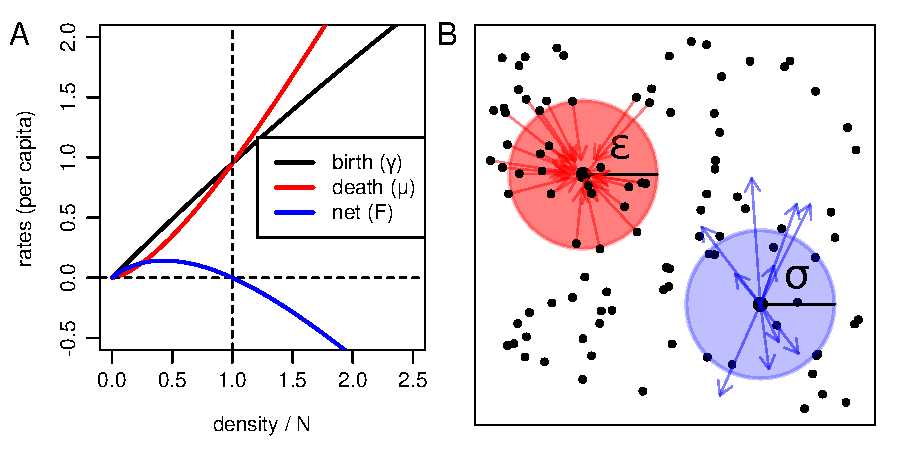
\includegraphics{figures/conceptual_figure}
    \end{center}
    \caption{
        \comment{Perhaps we should have two panels, one with the PME example (currently panel A) and the other with FKPP;
        right now panel B is not very helpful I think, so maybe should be omitted or added to so it better describes the whole process
        (including dispersal and establishment).}
        Conceptual figure of the model.
        \textbf{(A)} Example plot of $\gamma$, $\mu$, and $F$
        (calculated here with $r=1$) against scaled local population density.
        In this example, both birth and death rates increase with population density,
        but death increases faster,
        and equilibrium occurs where they cross
        (and hence where $F=0$).
        \textbf{(B)} Cartoon of interaction ($\epsilon$) and dispersal ($\sigma$) distances.
        \label{fig:model_setup}
    }
\end{figure}

Birth, establishment, and death can depend on the location of the individual
and the local population density.
Since we would like the population density to scale with $N$,
these are functions of $X/N$, i.e.,
the counting measure with mass $1/N$ placed at the location of each individual.
To measure local population density, we convolve the population measure with
an ``interaction kernel'' -- which, for simplicity, we take to be Gaussian,
and we write as
$$
    p_{\epsilon^2}(x) := \frac{1}{(2 \pi \epsilon^2)^{d/2}} e^{-\|x\|^2 / 2 \epsilon^2} ,
$$
for an ``interaction distance'' $\epsilon$.
First consider birth rates, defined by
a nonnegative function $\gamma(x, m) : \IR^d \times \IR_{\ge 0} \to \IR_{\ge 0}$
of location $x$ and local population density $m$,
and an interaction distance $\epsilon_\gamma > 0$.
Local population density enters through the convolution of $X$ with $p_{\epsilon_\gamma^2}$,
which we write as $\smooth{\gamma} X$.
Then, the birth rate of an individual at location $x$ when the state of the population is $X$
is $\gamma(x, \smooth{\gamma} X(x) / N)$.
Similarly, the establishment probability of an offspring at location $x$ is
is $r(x, \smooth{r} X(x) / N)$,
where $r(x, m) : \IR^d \times \IR_{\ge 0} \to [0, 1]$
and again $\smooth{r} X$ is the convolution of $p_{\epsilon_r^2}$ with $X$.
Rather than defining a function $\mu(x, m)$ for the death rate,
it turns out to be more convenient to parameterize in terms of the net reproductive rate,
which we denote by $F(x, m)$,
scaled by $1/\theta$
so that the population density changes over a time scale of $\theta$.
(This corresponds to a ``near-critical branching'' assumption.)
Informally, we would like that
$$
    F = \theta (r \gamma - \mu) ,
$$
and to arrange this we define
the death rate of an individual at $x$ to be
\begin{align} \label{eqn:mu_defn}
    \mu
    =
    \max\left\{0, 
        r(x, \smooth{r} X(x) / N) \gamma(x, \smooth{\gamma} X(x) / N)
        - \frac{1}{\theta} F(x, \smooth{F} X(x) / N)
    \right\} ,
\end{align}
where again $F(x, m) : \IR^d \times \IR_{\ge 0} \to \IR_{\ge 0}$
and $\kernel_F = p_{\epsilon_F^2}$.

In summary, each of the three demographic parameters depend on local density measured
with a Gaussian kernel with possibly different scales:
for birth over a scale of $\epsilon_\gamma$,
for establishment over a scale of $\epsilon_r$,
and for net reproductive rate over a scale of $\epsilon_F$.
Note that death rate depends in principle on population densities at three different scales,
so that we could write $\mu = \mu(x, \smooth{\gamma} X(x) / N, \smooth{r} X(x) / N, \smooth{F} X(x) / N)$.
It might seem like
we have introduced unnecessary complexity
with these three different spatial scales on which interactions occur.
However,
it will turn out to be useful in the proofs to have $\epsilon_r < \epsilon_\gamma$,
although in the limit they can be taken equal to each other
(and $\epsilon_F$ is unconstrained),
so informally we think of local density as being determined on a scale of $\epsilon$.

\begin{remark}
Although this model allows fairly general birth and death mechanisms,
there are a number of limitations.
Perhaps most obviously, to simplify the notation
individuals give birth to only one offspring at a time,
although this restriction could be easily lifted
\citep[as in Section 3.4 of][]{etheridge/kurtz:2018}.
Furthermore, individuals do not move during their lifetime,
and the age of an individual does not affect their fecundity or death rates.
Finally, there is no notion of mating
(although limitations on reproduction due to availability of mates can be incorporated into the birth rate, $\gamma$),
so the lineages we follow will be uniparental.
For these reasons, the model is most obviously applicable to bacterial populations or selfing plants,
although we do not anticipate that incorporation of these complications
will change the general picture.
\end{remark}

We next summarize the dynamics of the rescaled model $\eta(t) = X(\theta t)/N$,
and state some assumptions on the parameters.
The process takes values in the space of finite measures on $\IR^d$,
which we write as $\measures$.

\plr{TODO: check the conditions below (esp on the derivatives of $F$)}

\begin{definition}[Model parameterization and assumptions]
\label{def:model_setup}
Suppose $\gamma(x, m)$, $r(x, m)$, and $F(x, m)$
are uniformly continuous functions
from $\IR^d \times \IR_{\ge 0}$ to $\IR$.
Furthermore, suppose $r$ takes values in $[0, 1]$
and has uniformly bounded second derivatives,
that $\gamma(x,m) \ge 0$,
and that $m^2 \gamma(x, m)$ is uniformly bounded.
Fix positive values $\theta$, $\epsilon_r$, $\epsilon_\gamma$, and $\epsilon_F$,
with $\epsilon_r < \epsilon_\gamma$.
Suppose $F(x,m)$ is bounded above
with uniformly bounded first and second derivatives in $m$,
that $\sup_x F(x,m)$ is finite for all $m$,
and define
\begin{align} \label{eqn:mu_defn}
    \mu(x, \eta)
    =
    \max\left(0, 
        r(x, \smooth{r} \eta(x))
        \gamma(\smooth{\gamma} \eta(x))
        - \frac{1}{\theta}
        F(x, \smooth{F} \eta(x)) 
    \right) .
\end{align}
Although the models will make sense without this requirement,
for the purposes of convergence we will also require that
$\theta > 2 \sup_x \sup_{y : \|y\| = 1} y^T \covq(x) y/(\epsilon_\gamma^2 - \epsilon_r^2)$.
\end{definition}

Expressions like $\gamma(x, \smooth{\gamma} \eta(x))$ will appear often in the paper.
To make formula more readable, we overload notation to define
$$
    \gamma(x, \eta) := \gamma(x, \smooth{\gamma} \eta(x)) ,
$$
and similarly write $r(x, \eta)$ for $r(x, \smooth{r} \eta(x))$
and $\mu(x, \eta)$ for the expression of equation \eqref{eqn:mu_defn}.
When convenient, we may also suppress the arguments completely,
writing simply $\gamma$, $\mu$, and $r$ for these quantities.

For each value of $N$ and $\theta$,
the process $\left(\eta^N_t \right)_{t \ge 0}$
is the continuous-time measure-valued Markov process described above
with birth rates, establishment probabilities, and death rates
determined as follows.
When the state of the process is $\eta \in \measures$,
offspring of mass $1/N$ are produced at location $x$
with rate $\theta \gamma(x, \eta) N \eta(dx)$
and adults die at location $x$ with rate $\theta \mu(x, \eta) N \eta(dx)$,
(i.e., at rates $\theta \gamma$ and $\theta \mu$ per capita respectively).
Each offspring disperses to a location offset from the parent's location
by an independent Gaussian with mean $\meanq(x) / \theta$
and covariance matrix $\covq(x) / \theta$;
an offspring at $x$ establishes instantaneously
with probability $r(x, \eta)$, or else dies.

We have just effectively defined the process, but for future use,
we will now give a formal definition as a solution to a martingale problem.

\begin{definition}[Martingale Problem Characterisation]
    \label{defn:mgale_construction},
For each value of $N$ and $\theta = \theta(N)$,
we define $(\eta^N_t)_{t \geq 0}$ to be the solution to the Martingale Problem,
with initial condition $\eta^N_0 \in \measures$,
such that for all smooth functions $f \in C^{\infty}_{0}(\IR^d)$,
writing $\langle f, \eta \rangle = \int_{\IR^d} f(x) \eta(dx)$
and $q_\theta(x, dy)$ as the Gaussian kernel
with mean $x + \meanq(x)/\theta$ and covariance $\covq(x) / \theta$,
\begin{equation}
    \label{eqn:eta_martingale}
\begin{aligned}
M^N_t(f)
&:=  \langle f, \eta^N_t \rangle
        -\langle f, \eta^N_0 \rangle
 \\ &\qquad {}
 -  \int_{0}^{t}\bigg\{
        \int\left( \int \theta
             \left(
                f(z)r(z, \eta^N_{s})
                - f(x)r(x, \eta^N_{s})
            \right)
        q_\theta(x,dz) \right)
\\ & \qquad \qquad \qquad \qquad {}
        \times \gamma(x, \eta^N_{s}) \eta^N_{s}(dx)
\\ & \qquad \qquad {}
    + \int f(x) F(x, \eta^N_{s}) \eta^N_{s}(dx)
    \bigg\} ds
\end{aligned}    
\end{equation}
is a martingale with quadratic variation
    \begin{equation} \label{eqn:prelimit_martingale_variation}
\begin{aligned} \relax
[ M^N_t(f)] =& 
\frac{\theta}{N} \int_{0}^{t}\bigg\{
    \langle \gamma(x, \eta^N_{s})
        \int f^2(y)r(y, \eta^N_{s}) q_\theta(x,dy) 
    , \eta^N_{s}(dx) \rangle \\
& \qquad \qquad {}
    + \langle \mu(x, \eta^N_{s}) f^2(x) 
    , \eta^N_{s}(dx)\rangle
    \bigg\}ds. 
\end{aligned}    
\end{equation}
\end{definition}

Note that
since individuals are produced at rate $N \gamma \eta$ but have mass $1/N$ each,
these factors of $N$ cancel in~\eqref{eqn:eta_martingale}.
Since we are taking a diffusion limit,
we will have use for the following notation:

\begin{definition}[Dispersal generator]
    \label{def:dispersal_generator}
    Recall that we have defined the dispersal kernel,
    $q_\theta(x, dy)$,
    to be the density of a multivariate Gaussian
    with mean $\meanq(x)/\theta$ and covariance matrix $\covq(x)/\theta$
    (although sometimes we omit the dependence of $\meanq$ and $\covq$ on $x$).
    This implies that if we define, for $f : \IR^d \to \IR$,
    \begin{align}
    \DG f(x)
        =
        \sum_{ij} \covq(x)_{ij} \partial_{x_i} \partial_{x_j} f(x)
        + \sum_i \meanq(x)_i \partial_{x_i} f(x)
    \end{align}
    then
    \begin{align}
        \theta \int \left(
            f(y) - f(x)
        \right) q_\theta(x, dy)
    \to \DG f(x) 
        \qquad \text{as } \theta \to \infty .
    \end{align}
    We will also denote the adjoint of $\DG$ by
    \begin{align*}
    \DG^* f(x)
        &=
        \sum_{ij} \partial_{x_i} \partial_{x_j} (\covq(x)_{ij} f(x))
        - \sum_i \partial_{x_i} (f(x) \meanq(x)_i) 
        \\
        &=
        \text{TODO} .
    \end{align*}
\end{definition}

\paragraph{Remark:}
An equivalent way to describe the model would be to say that
when the state of the population is $\eta$,
an individual at $x$ gives birth at rate
$$
    \theta \gamma(x, \smooth{\gamma} \eta(x))
    \int r(y, \smooth{r} \eta(y)) q(x, dy) ,
$$
and that offspring disperse according to the kernel
$$
    q_\theta^\mathfrak{m}(x,\eta,  dy)
    :=
    \frac{
        r(y, \smooth{r} \eta(y)) q_\theta(x, dy)
    }{
        \int r(z, \smooth{r} \eta(z)) q_\theta(x, dz)
    } .
$$
Clearly, the random walk driven by this dispersal kernel
is biased towards regions of higher establishment probability.
For comparison to future results,
it is interesting to write down the limiting generator:
\begin{align*}
    \lim_{\theta \to \infty}
    \theta \int (f(y) - f(x)) q_\theta^\mathfrak{m}(x, \eta, dy)
    &=
    \frac{
        \DG\left[ f(\cdot) r(\cdot, \smooth{r} \eta(\cdot)) \right](x)
        - 
        f(x) \DG\left[ r(\cdot, \smooth{r} \eta(\cdot)) \right](x)
    }{
        r(x, \smooth{r} \eta^{N}(x))
    } .
\end{align*}
In the simplest case of unbiased, isotropic dispersal,
$\meanq = 0$ and $\covq = I$, so $\DG = \Delta$,
and this is equal to
\begin{align*}
    \Delta f(x) + 2 \grad f(x) \cdot \grad \log r(\cdot, \smooth{r} \eta(\cdot))(x) .
\end{align*}
One might guess that the spatial motion described by following a lineage of successful individuals back through time
would be described by this generator in the limit.
However, we will see that following a lineage back through the population
has a different behavior yet again.


% % % % % % % % % % % % % % %
\subsection{Scaling limits of the population density process}

Our main results depend on two dichotomies:
Is the limiting process deterministic or a (generalized) superprocess?
And, are interactions local in the limit or not?
Below we have results for deterministic limits with local and nonlocal interactions,
and for superprocess limits with nonlocal interactions.
See Figure \ref{fig:super_vs_det_2d} for illustrative simulations.
We suspect that limits are possible in the remaining (local, superprocess) case
only in $d=1$, but do not discuss the case further.


\begin{figure}
    \begin{center}
        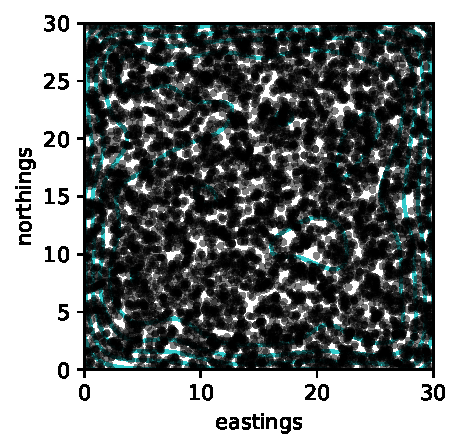
\includegraphics{figures/ex1a/fkpp_123.locations}
        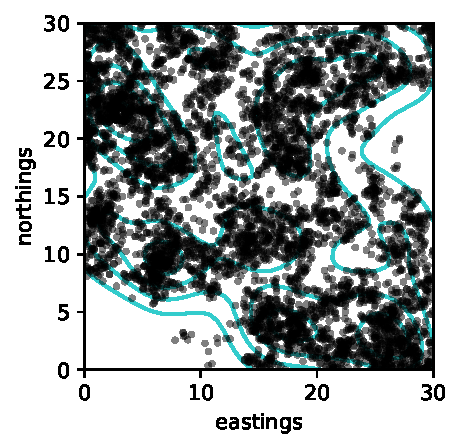
\includegraphics{figures/ex1b/fkpp_123.locations}
    \end{center}
    \caption{
        Snapshots of two simulations, with small $\theta$ (left) and large $\theta$ (right).
        Simulations are run with a FKPP-like parameterization:
        birth and establishment are constant, while death increases linearly with density,
        at slope $1/\theta$.
        Left: $\theta=1$. Right: $\theta=100$.
        Other parameters were the same:
        dispersal and interactions distance were set to 1,
        and the equilibrium density is 10 individuals per unit area.
        \label{fig:super_vs_det_2d}
    }
\end{figure}

\begin{theorem} \label{thm:nonlocal_convergence}
    Let $(\eta^N_t)_{t \geq 0}$
    be as defined in Definition \ref{def:model_setup}
    and assume that as $N \to \infty$, also $\theta \to \infty$
    in such a way that $\theta/N \to \alpha$.
    (However, interaction distances $\epsilon_r$, $\epsilon_\gamma$, and $\epsilon_F$
    remain constant.)
    The sequence of stochastic processes
    $(\eta^N_t)_{t \geq 0}$
    converges along subsequences in distribution as $N \to \infty$
    to a measure-valued process $(\eta_t)_{t \geq 0}$
    which satisfies that, for every $f \in C^\infty_0(\IR^d)$,
    \begin{align} \label{eqn:limiting_mgale_problem}
        \begin{split}
        M_t
            &:=
            \langle f(x), \eta_t(dx) \rangle
            -
            \langle f(x), \eta_0(dx) \rangle
            \\ & \qquad
            -
            \int_0^t \big\langle
                \gamma(x, \eta_s)
                \mathcal{B}\left(
                    f(\cdot) r(\cdot, \eta_s)
                \right)(x)
                \\ &\qquad \qquad \qquad {}
                +
                f(x)
                F(x, \eta_s),
                \eta_{s}(dx)
            \big\rangle ds,
        \end{split}
    \end{align}
    is a martingale,
    with quadratic variation
    \begin{align} \label{eqn:limiting_mgale_variation}
        [ M ]_t
        =
        \alpha
        \int_0^t
        \big\langle
            \left(\gamma\left( x, \eta_{s} \right)
            r\left(x, \eta_{s} \right) + \mu\left(x, \eta_{s} \right)\right)
            f^2(x),
            \eta_{s} (dx)
        \big\rangle ds. 
    \end{align}
    In other words, the limit is a measure-valued process with non-local interactions.
    Furthermore, if $\alpha = 0$ the limit is deterministic.
\end{theorem}

Recall when interpreting~\eqref{eqn:limiting_mgale_problem}
that for instance $r(x, \eta_s) = r(x, \smooth{r} \eta_s(x))$,
and so $\DG(fr)(x) = \DG(f(\cdot) r(\cdot, \smooth{r} \eta_s(\cdot)))(x)$.

Theorem \ref{thm:nonlocal_convergence} provided convergence along subsequences;
i.e., for any sequence of values of $N$
there is a subsequence along which $\eta^N$ converges.
However, if the limiting process is unique then the convergence is unqualified.
In the deterministic case, we have convergence to a nonlocal PDE.

\begin{corollary}[Superprocess limits] \label{cor:superprocess_uniqueness}
    Under the assumptions of Theorem~\ref{thm:nonlocal_convergence},
    if the martingale problem
    defined by equations \eqref{eqn:limiting_mgale_problem} and \eqref{eqn:limiting_mgale_variation}
    has a unique solution,
    then $(\eta^N_t)_{t \ge 0}$ converges to that solution
    as $N \to \infty$.
    \comment{
        Is this what we want to say here? Could be said better.
        TODO: see what Dawson \& Li say about uniqueness
        so we have at least some conditions under which this happens.
    }
\end{corollary}

\comment{
    TODO: put in what Kurtz \& Xiong have to say about uniqueness,
along the lines of a note saying ``For some conditions under which the limit is known to be unique,
see Kurtz \& Xiong and/or Dawson \& Li.''
}

Our results will show that in deterministic limits ``$\eta_t$ solves a PDE'',
but since $\eta_t$ is a measure for which we don't always know there exists a density,
we need to formalize the weak sense in which it solves the PDE.
The notation in the following definition
is written to suggest the case in which $\eta_t(dx)$ has a density $\varphi_t(x)$.

\begin{definition}[Weak solutions]
    \label{defn:weak_solutions}
    We say that $(\eta_t)_{t \ge 0}$, with $\eta_t \in \measures$
    is a \emph{weak solution} to the PDE
    $$
        \dot \varphi = r \DG^*(\gamma \varphi) + \varphi F
    $$
    if for all $f \in C_0^\infty(\IR^d)$,
    $$
        \frac{d}{dt} \langle f, \eta_t \rangle
        =
        \langle
            \gamma \DG(rf) + f F,
            \eta_t
        \rangle .
    $$
    \comment{Write this out with $(x)$'s?}
\end{definition}


\begin{corollary}[Deterministic limits]
    \label{cor:nonlocal_pde_limits}
    Under the assumptions of Theorem~\ref{thm:nonlocal_convergence},
    if the limit is deterministic (i.e., $N^{-1}\theta \to \alpha = 0$),
    then any limit $\eta_t$ is a weak solution to the nonlocal partial differential equation
    \begin{equation} \label{eqn:nonlocal_pde}
        \partial_t \varphi_t(x)
        =
        r\left(x, \smooth{r} \varphi_t(x) \right)
        \DG^* \left[
            \varphi_t(\cdot)
            \gamma\big( x, \smooth{\gamma} \varphi_t(\cdot) \big)
        \right](x)
        +
        \varphi_t(x)
        F\left(x, \smooth{F} \varphi_t(x) \right)
        ,
    \end{equation}
    in the sense of Definition~\ref{defn:weak_solutions}.
    If equation \eqref{eqn:nonlocal_pde} has a unique solution,
    then $(\eta^N_t)_{t \ge 0}$ converges to that solution.
\end{corollary}

\comment{TODO: Tom has conditions, referring to \citet{KURTZ1999103}, (coefficient are Lipschitz?) under which
    the solution to \eqref{eqn:nonlocal_pdf} is unique and has a density (Thm 2.1 in DDMOT);
    insert those here (as a Corollary or Proposition)}

Informally, equation \eqref{eqn:nonlocal_pde} is the PDE of Definition~\ref{defn:weak_solutions},
where $\DG$ is an elliptic second order differential operator,
and the coefficients $r$, $\gamma$, and $F$
at $x$ depend nonlocally on $\varphi$
(i.e., through a smoothed version of $\varphi$).
To see why it is $\DG^*$ and not $\DG$ that appears in this equation,
consider the case where dispersal has a mean drift to the right,
so that the drift term in $\DG$ is $d/dx$.
Then, the population density at a location with positive slope
will tend to \emph{decrease}, i.e., proportional to $-d/dx$,
because the density at a location is determined by the offspring that disperse \emph{to}
that location, not away from it.
Furthermore, if dispersal tends to move offspring away from a region
(i.e., if divergence $\grad \cdot \meanq > 0$)
this will tend to decrease the local density.

Although the coefficients at $x$ in \eqref{eqn:nonlocal_pde} are nonlocal,
they depend only on the region nearby to $x$,
and so we would expect solutions of the nonlocal PDE to be close to the corresponding local PDE
as the interaction distances $\epsilon_r$, $\epsilon_\gamma$ and $\epsilon_F$
go to zero:
for instance, if $\eta_t$ has density $\varphi_t$
then $\gamma(x, \smooth{\gamma} \eta_t(x)) \to \gamma(x, \varphi_t(x))$ as $\epsilon_\gamma \to 0$
(recalling that $\smooth{\gamma}{}$ denotes convolution with the heat kernel at time $\epsilon_\gamma^2$).
The following propositions give two concrete situations in which that is true.

\begin{proposition}
    \label{prop:nonlocal_to_local}
    Suppose that $\eta^\epsilon_t$ is a weak solution to equation \eqref{eqn:nonlocal_pde}
    with $r(x, m) = 1$ for all $x$ and $m$
    and some $\epsilon_r + 1/\theta < \epsilon_\gamma = \epsilon_F = \epsilon$
    \comment{and assumptions on $\gamma$? and $F$?}.
    Then $\eta^\epsilon_t(dx)$ converges \comment{in what sense?} as $\epsilon \to 0$
    to $\varphi_t(x) dx$, which is a (strong) solution to
    \begin{align} \label{eqn:PDE}
        \partial_t \varphi(t, x)
        =
        \DG^* \left( \gamma(\cdot, \varphi(t, \cdot)) \varphi(t, \cdot)  \right)(x)
        + F(x, \varphi(t, x)) \varphi(t, x) .
    \end{align}
\end{proposition}

Theorem \ref{thm:nonlocal_convergence} combined with Proposition \ref{prop:nonlocal_to_local}
imply that we can take the $N \to \infty$ limit
followed by $\epsilon \to 0$
to obtain solutions to the PDE \eqref{eqn:PDE}.
However, it is of substantial interest to know whether
we can take those two limits simultaneously.
The general case seems difficult,
but we can prove such ``diagonal'' convergence in the following situation.

\begin{theorem}[Convergence to a PDE]
    \label{thm:local_convergence}
    Let $(\eta^N_t)_{t \geq 0}$
    be as defined in Definition \ref{def:model_setup}
    and assume that as $N \to \infty$, $\theta \to \infty$
    and $\epsilon_r + 1/\theta < \epsilon_\gamma = \epsilon_F = \epsilon \to 0$
    in such a way that $\theta/N \to 0$
    and
    \comment{TODO: some conditions on $\epsilon$ and $r$ and $\gamma$ and $F$}.
    Then the sequence of stochastic processes $(\eta^N_t)_{t \ge 0}$
    converges \comment{in some sense}
    to a measure-valued process with a density $\varphi(t, x)$
    that solves
    \begin{align}
        \partial_t \varphi(t, x)
        &=
        \text{whatever the final form is here} .
    \end{align}
\end{theorem}


% % % % % % % % % % % %
\subsection{Ancestral lineages in the scaling limit}

Now that we have established what we can say about how population density changes with time,
we turn to results on ancestral lineages,
i.e., how genealogical ancestry can be traced back across the landscape.
Informally,
a \emph{lineage} $(L_t)_{t \ge 0}$
begun at spatial location $L_0 = x$
can be obtained by picking a focal individual uniformly at $x$,
and then for each amount of time $t$ in the past,
setting $L_t$ to the spatial location of the individual from whom
the focal individual inherits at that time in the past.
Since in our model individuals have only one parent, this is unambiguous.
Although we did not explicitly retain such information,
it is clear that for finite $N$
one could construct the distribution of a lineage $(L_t)_{t=0}^T$
given the history of the population $(\eta^N_t)_{t = 0}^T$,
for each starting location to which $\eta^N_T$ assigns positive mass.
It is less clear, however, how to formally retain such information in the limit.
The \emph{lookdown construction} in Section~\ref{sec:lookdown}
provides just such a construction.
Roughly speaking,
this works by assigning to each particle a unique ``level''
that functions as a label and thus allows reconstruction of lineages,
but also (in some sense) orders individuals by eventual reproductive output,
allowing a formal limit.
See~\citet{etheridge/kurtz:2018} for an introduction to these ideas.

A lineage is, in general, a well-defined stochastic process,
but there are two important questions
that affect its tractability.
First, when is it a Markov process given the population process?
(In other words, given $(\eta_t)_{t=0}^T$ that records numbers of individuals
but not their ancestry.)
\comment{NOT RIGHT:}
We expect the answer here to be that a lineage is Markov
only in the $N \to \infty$ limit
(see \citet{barton/depaulis/etheridge:2002} for discussion).
Second, does the process have a tractable description?
If the population process has a density,
then it turns out that a lineage is a diffusion driven by the density.
The remaining case is the superprocess limit ($\theta/N \to \alpha > 0$);
in this case, we expect that a lineage could still be described as a generalized diffusion,
but moving within a stochastic landscape that is singular in $d \ge 2$.
We focus on the more tractable situation where the population process is deterministic.
However, the results here apply to either the local or nonlocal case
(i.e., where the density solves a local or nonlocal PDE).


\begin{definition}[Generator of a lineage] \label{def:lineage_generator}
    Let $(\varphi_t(x))_{0 \le t \le T}$
    denote the density of a population that solves \eqref{eqn:nonlocal_pde},
    and let $y$ be a point with $\varphi_T(y) > 0$.
    We define $(L_s)_{s=0}^T$,
    the ancestral lineage in this population of an individual sampled at $y$ at time $T$,
    to be the position of the unique ancestor of $y$ alive at time $T - s$.
    We define
    $(Q_s)_{s \geq 0}$
    to be the time inhomogeneous semi-group satisfying
    \begin{align*}
        Q_s f(y) := \IE_y[ f(L_s) ] .
    \end{align*}
\end{definition}

Our main result identifies a lineage as a diffusion
by characterizing its generator.


\begin{theorem} \label{thm:lineages}
    For $\varphi: \IR^d \to \IR$, define
    \begin{align}
        \label{eqn:lineage_generator}
        \Lgen_\varphi f
        &=
        \frac{r}{\varphi}
        \left[
            \DG^*(\gamma \varphi f) 
            - f \DG^* (\gamma \varphi)
        \right] \\
        &= \label{eqn:lineage_generator2}
        r\gamma
        \left[
            \sum_{ij} \covq_{ij} \partial_{ij} f
            + \sum_j \vec{m}(s)_j \partial_j f
        \right] ,
    \end{align}
    where $\vec{m}$ is the vector
    $$
    \vec{m}(s)_j
    =
    2 \sum_i C_{ij} \partial_i \log(\gamma \varphi)
    + 2 \sum_i \partial_i C_{ij}
    - \meanq_j .
    $$
    Then $\Lgen_{\varphi_{T-s}}$ is the generator of the semigroup $Q_s$
    of Definition~\ref{def:lineage_generator}.
\end{theorem}

As usual,
to make the generator readable, we've written it in concise notation,
omitting the dependencies on location and population density,
which itself changes with time.
When interpreting this,
remember that everything depends on location and density at that location and time --
for instance, ``$r$'' is actually $r(x, \varphi(x))$ (in the local case),
or $r(x, \smooth{r} \eta(x))$ (in the nonlocal case).

\begin{corollary} \label{cor:lineages_simple}
    In addition to the assumptions of Theorem~\ref{thm:lineages},
    if the dispersal process is isotropic
    (i.e., $\covq = \sigma^2 I$ and $\meanq$ is constant),
    then
    \begin{equation}
        \Lgen_\varphi f
        =
        r \gamma
        \left(
            \sigma^2 \Delta f
            +
            \left(
                2 \sigma^2 \grad \log(\gamma \varphi)
                - \meanq
            \right)
            \cdot \grad f
        \right) .
    \end{equation}
\end{corollary}

In other words, 
the lineage behaves as a diffusion driven by Brownian motion run at speed 
\comment{TODO: make this right:}
If $V_s(x) = \log(\varphi_s(x) \gamma(x, \varphi_s)) - \meanq \cdot x / 2 \sigma^2$,
then the diffusion has drift $\grad V_s$.
If $\varphi$ does not change with time, 
then the stationary distribution is proportional to $\exp(V(x))$.
a lineage behaves as a diffusion
that is driven by a Brownian motion 
run at speed $\sigma^2$ multiplied by the local per-capita production of offspring ($r \gamma$)
in a potential equal to the local birth output tilted by migration bias
($\varphi_s \gamma \exp(-\meanq \cdot x / 2 \sigma^2)$).


\begin{corollary} \label{cor:wavefront}
    In addition to the assumptions of Corollary~\ref{cor:lineages_simple},
    suppose that the population process is described by a traveling wave with speed $\wavespeed$,
    i.e., the population has density
    $\varphi(t, x) = w(x - t \wavespeed)$
    where $w$ solves
    \begin{align*}
        r \Delta (\gamma w) + w F + \wavespeed \cdot \grad w = 0 .
    \end{align*}
    Then the semigroup 
    of the motion of a linages in this population 
    $Q_s$ is time-homogeneous with generator
    \begin{align}
        \Lgen f
        &=
        \sigma^2 r \gamma
        \left(
            \Delta f
            +
            2 \grad \log (\gamma w)
            \cdot \grad f
        \right)
        + (\wavespeed - \meanq) \cdot \grad f .
    \end{align}
\end{corollary}


%%%%%%%%%%%%%%%%%%%%%%
\section{Examples and applications}
\label{sec:applications}

Next,
we cover some illustrative examples
and interesting applications.

% % % % % % % % % % % %
\subsection{Beyond reaction-diffusion equations: a population described by the porous medium equation}
\comment{look up what the technical term is for the nonlinear diffusive bit?
    and, does "reaction-diffusion" mean parabolic?}

Consider the porous medium equation (PME) with logistic growth,
\begin{equation}
    \label{eqn:pme}
    \partial_t v = \partial_x^2 (v^2) + v (1 - v) ,
\end{equation}
an example of a reaction-diffusion equation with a nonlinear diffusion term.
Such equations are widely used in a number of contexts in biology in which
it is clear that motility within a population varies with population density.
For example, density dependent dispersal is a common feature in spatial
models in ecology, eukaryotic cell biology, and avascular tumour growth;
see~\cite{sherratt:2010} and references therein for further discussion. 
In particular, it has been suggested as a model for
the expansion of a certain type of bacteria % of the type {\em Paenbacillus dendritiformis}
on a thin layer of agar in a petri dish 
\citep{cohen/golding/kozlovsky/benjacob/ron:1999}. 
We shall pay particular attention to the case in which the equation can be 
thought of as modelling the density of an expanding population. 

Comparing \eqref{eqn:pme} to \eqref{eqn:pde},
we see that to set up a limit in which the population density $\varphi$ follows the PME,
we need $r=1$,
$\gamma = \varphi$, and $F = 1 - \varphi$.
Consulting equation~\eqref{eqn:mu_defn},
this implies that $\mu = (1 + 1/\theta) \varphi - 1/\theta$.
In other words,
establishment is certain
and birth rates increase linearly with population density,
but to compensate, death rates increase slightly faster (also linearly),
as shown in Figure~\ref{fig:pme_waves}.
Alert readers will notice that
for finite $\theta$ death rates may be negative,
and furthermore rates are not bounded;
in practice we choose a suitably small value for $\beta$ and define
\begin{align*}
    \gamma(x, m) &= (1 - \exp(- \beta m)) / \beta \\
    F(x, m) &= \exp(- \beta m) / \beta ,
\end{align*}
and set $\mu(x, m) = \max(0, \gamma - F / \theta)$.
Birth and death rates are equal at density $m = 1$,
corresponding to an unscaled density of $N$ individuals per unit area.

\begin{figure}
    \begin{center}
        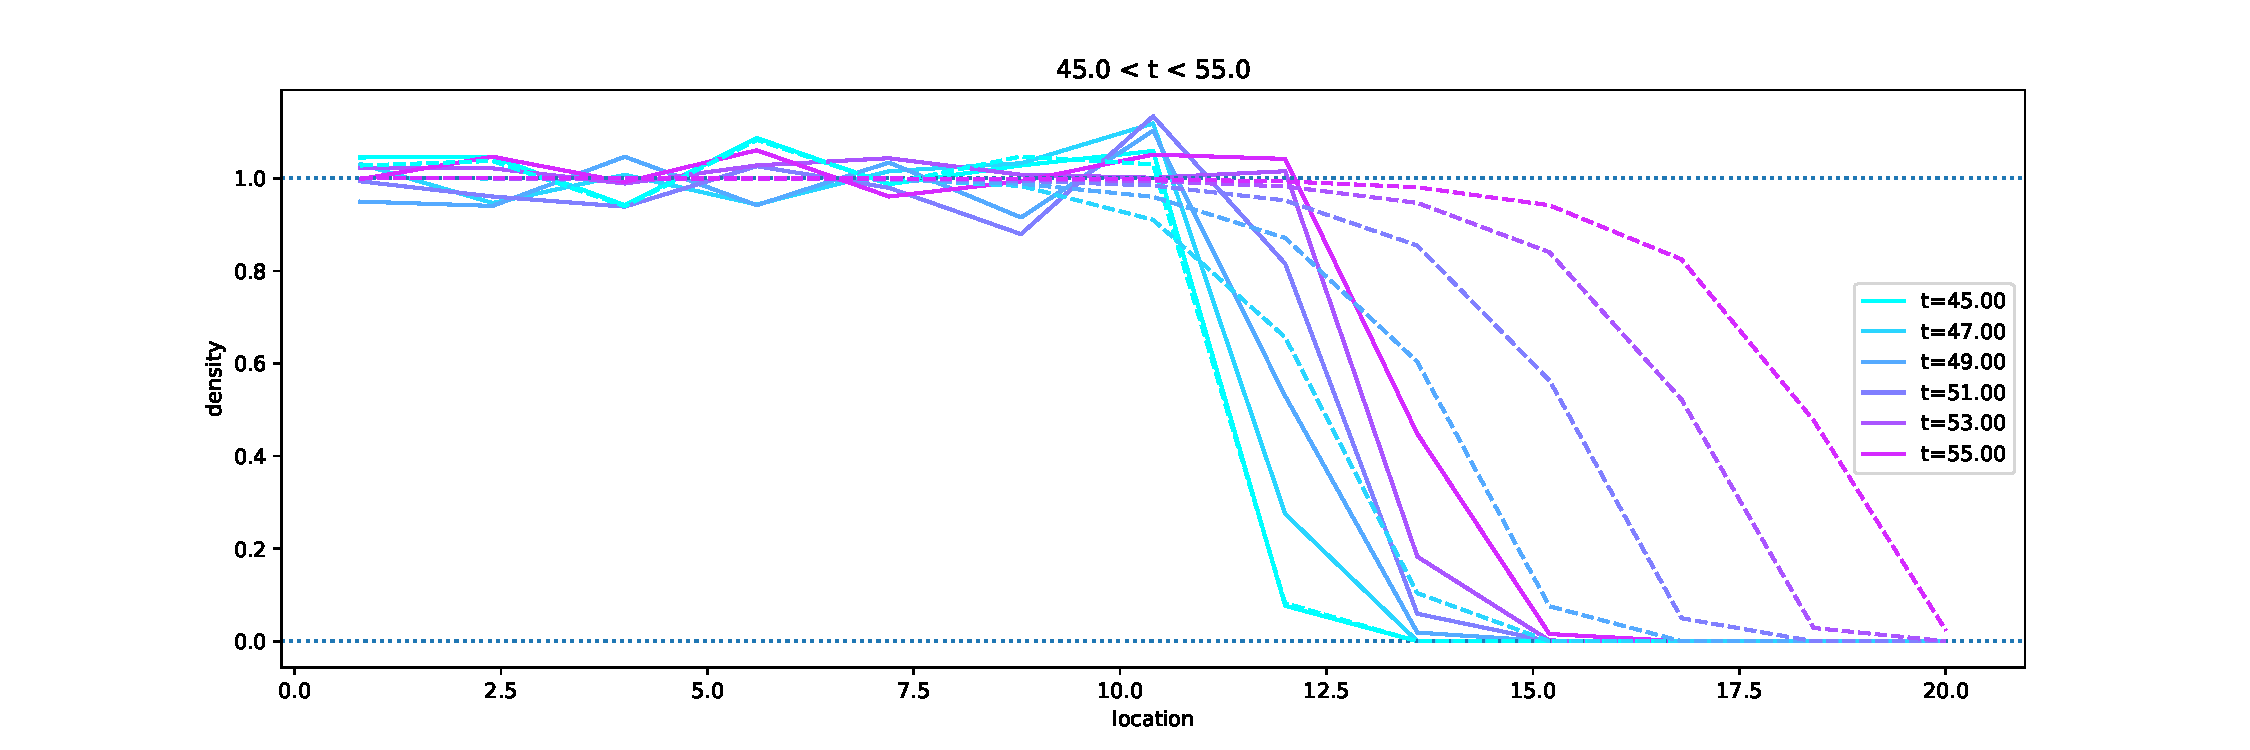
\includegraphics[width=0.45\textwidth]{figures/ex2a/pme_123.steps}
        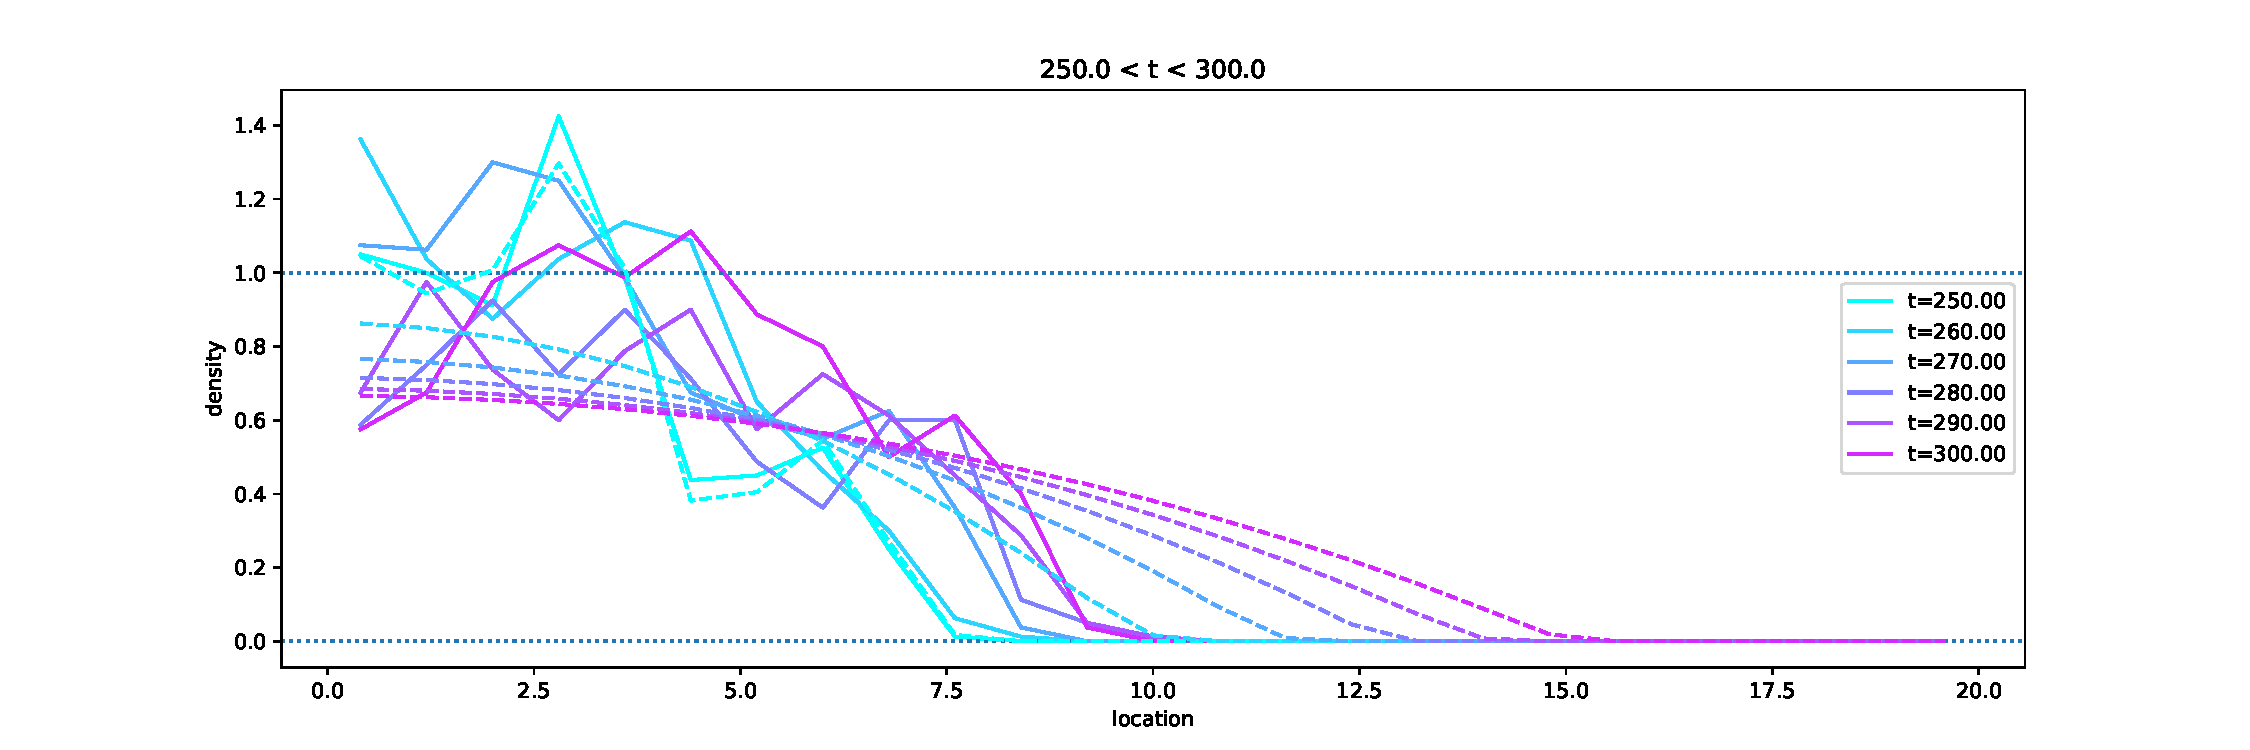
\includegraphics[width=0.45\textwidth]{figures/ex2b/pme_123.steps}
    \end{center}
    \caption{
        Two panels, showing simulated 1D populations under the PME, comparing the simulated
        profile to the analytical solution;
        $\theta/N$ not small on left; small on right.
        (Note: noisier wave should move slower, we'll see this.)
        \label{fig:pme_waves}
    }
\end{figure}

This equation has an explicit travelling wave solution
\begin{align} \label{eqn:pme_wave}
    w^P(t, x)
    :=
    \left( 1 - e^{ \frac{1}{2} (x - x_0 - t) } \right)_+ .
\end{align}
Notice that the wave profile has a sharp boundary at $x = x_0 + t$.
There are also travelling wave solutions with $c>1$ \citep{gilding/kersner:2005},
which lack this property.
However, for initial conditions that decay sufficiently rapidly at infinity,
such as one might use in modelling a population invading new territory,
the solution converges to \eqref{eqn:pme_wave} \citep{kamin/rosenau:2004}.

Indeed, simulations of this process
shown in Figure~\ref{fig:pme_waves}
display traveling wave solutions
similar to numerical solutions of the PME,
with increasingly good agreement for larger $\theta$ and $N$.
As expected, noise slows down the wave.


% % % % % % % % % % % %
\subsection{Different types of traveling waves}

\begin{figure}
    \begin{center}
        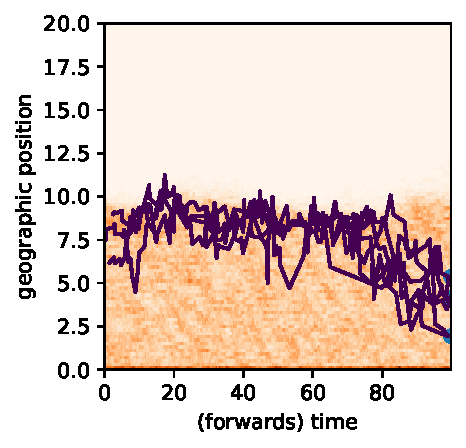
\includegraphics{figures/ex3_fkpp/fkpp_123.lineages}
        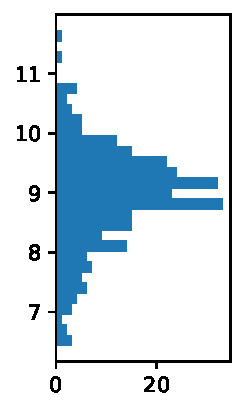
\includegraphics{figures/ex3_fkpp/fkpp_123.lineagehist}
        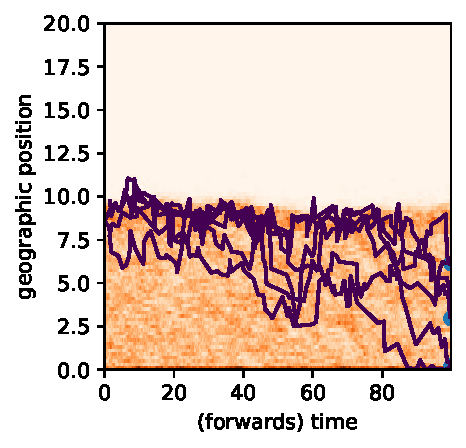
\includegraphics{figures/ex3_pme/pme_123.lineages}
        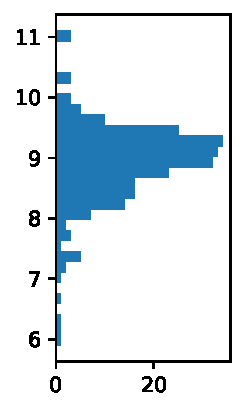
\includegraphics{figures/ex3_pme/pme_123.lineagehist}
        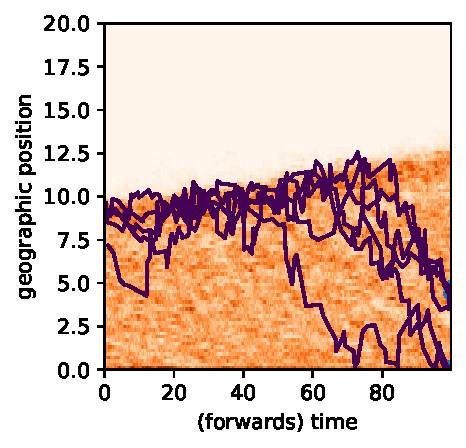
\includegraphics{figures/ex3_allen-cahn/allen-cahn_123.lineages}
        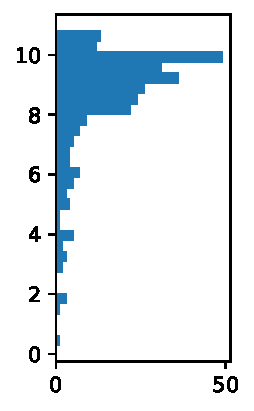
\includegraphics{figures/ex3_allen-cahn/allen-cahn_123.lineagehist}
    \end{center}
    \caption{
        Six panels: one pair for FKPP, one for PME, and one for Allen-Cahn.
        Each pair shows (top) lineage traced back in wavefront,
        and (bottom) stationary distribution of lineage location,
        compared to analytical solution for PME.
        \label{fig:pme_vs_fkpp}
    }
\end{figure}

It is interesting to investigate the motion of an ancestral lineage
in special cases in which we have an explicit expression for the travelling
wave profile $w$. 
We consider three relatively well-studied examples:
the Porous Media equation (above),
the Fisher-KPP equation,
and the Allen-Cahn equation.
We will work here in one dimension,
and take $\sigma^2 = 1$ and $\meanq = 0$.

%%%%%%%%%%
\paragraph{Porous Media:}
Setting $x_0=0$ (for definiteness) and substituting
the form of $w^P$ from equation \eqref{eqn:pme_wave}
into Corollary~\ref{cor:wavefront},
with $c=1$,
$\gamma(x, m) = m$,
$r(x,w) = 1$,
and $F(x, m) = (1 - m)$,
the lineage's generator is, for $x < 0$,
with $f_x$ denoting the spatial derivative of $f$,
\begin{align*}
    \Lgen f
    &=
        w(x)
        \left(
         f_{xx}(x)
         +
         2 \frac{(w(x)^2)_x}{w(x)^2} f_x(x)
        \right)
        + f_x(x) \\
    &=
        \left(1 - e^{\frac{1}{2} x} \right)
        f_{xx}(x)
        -
        2 e^{\frac{1}{2} x} f_x(x)
        +
        f_x(x) .
\end{align*}
The speed measure corresponding to this diffusion is,
again for $x < 0$,
\begin{align*}
    m(d\xi)
    &\propto
        \frac{ 1 }{ 2 (1 - e^{\xi/2}) }
        \exp\left(
            \int_\eta^\xi \left\{
                1 - \frac{e^{x/2}}{1 - e^{x/2}}
            \right\} dx
        \right) \\
    &\propto
        e^\xi\left(1-e^{\xi/2}\right),
        \quad
        \text{for } \xi < 0 ,
\end{align*}
which is integrable and so when suitably normalised gives the unique stationary distribution.
Notice that at stationarity
the lineage will typically be significantly behind the front. 

%%%%%%%%%%
\paragraph{Fisher--KPP:}
A great deal more attention has been paid to the classical Fisher-KPP equation,
\begin{align} \label{eqn:fkpp}
    v_t = v_{xx} + v (1-v) .
\end{align}
Even though we do not have an explicit formula for the wave shape in this case,
our methods provide information about ancestral lineages.
The equation has non-negative travelling wave solutions of speed $c$ for all $c \geq 2$, 
but started from any compact perturbation of a Heaviside function, the 
solution will converge to the profile $w^F$ with the minimal wavespeed, $c=2$
\citep{kolmogorov/petrovsky/piscounov:1937,bramson:1983}.
No matter the initial condition,
for any $t>0$ the support of the 
solution will be the whole real line. 
In this case, we must have $r = \gamma = 1$,
and $F(x, m) = 1 - m$ so $\mu(x, m) = 1 + (m-1)/\theta$.
This implies that
the generator of the motion of an ancestral lineage is
\begin{equation} \label{eqn:fkpp_generator}
    \Lgen \phi
    =
    \phi_{xx} + 2 \frac{w_x}{w} \phi_x + 2 \phi_x .
\end{equation}
Near the tip of the wave (for $x$ large), $w^F(x) \sim e^{-x}$,
so \eqref{eqn:fkpp_generator} implies that
the motion of a lineage is close to unbiased Brownian motion.
On the other hand, for $x < 0$ a lineage behaves approximately as
Brownian motion with drift at rate two to the right.
This implies that
ancestral lineages are pushed into the tip of the wave,
and there is no stationary distribution,
so that long-term dynamics of genetic inheritance
depend on the part of the wave not well-approximated by a smooth profile.
These results agree with those of \comment{TODO: citations}.


%%%%%%%%%%
\paragraph{Allen-Cahn:}
Finally, we take the Allen-Cahn equation
\begin{align} \label{eqn:allen_cahn}
    v_t = v_{xx} + v(1-v)(2v-1+s),
\end{align}
for a given $s \in (0,2)$,
which is used to model populations evolving under selection \cite{Sarah}.
This equation also has an explicit travelling wave solution with speed $s$
and shape
\[ w^A(x) = (1+e^{x})^{-1}. \]
The generator for ancestral lineages is, just as in the Fisher-KPP case,
\begin{align*}
    \hat{\mathcal{L}}\phi
    &=
    \phi_{xx}
    + 
    2 \frac{w_x}{w} \phi_x
    +
    s \nabla \phi \\
    \qquad &=
    \phi_{xx}
    -
    2 \frac{e^x}{1+e^x} \phi_x 
    + 
    s \nabla \phi,
\end{align*}
so lineages in the tip are pushed leftwards into the bulk of the wave at a rate $-2(e^{-x}+1)^{-1}$,
that gets weaker further to the left.
This diffusion has speed measure
$$
    m(d\xi) \propto e^{sx}(1+e^x)^{-2},
$$
which is concentrated around $\log(s/(2-s))$ and decays like $e^{x(s-2)}$ away from this point.
These results agree with those of \cite{etheridge/penington:2020}.


% % % % % % % % % % % % % % % %
\subsection{Clumping from nonlocal interactions}

\comment{
    Description of the process;
    discussion of when it happens;
    (TODO: how's it affected by $\theta$?)
}

\begin{figure}
    \begin{center}
        FIGURE
    \end{center}
    \caption{
        Two panels: left is 2D picture of clumped population;
        right is a bumpy expanding wavefront.
        \label{fig:clumping}
    }
\end{figure}


% % % % % % % % % % % % % % % %
\subsection{Lineage motion is not uniquely determined by population density}

It is natural for applications to wonder about identifiability:
when can the observed quantities like population density
or certain summaries of lineage movement uniquely determine
the underlying demographic parameters?
Consider a deterministic,
continuous population generated by parameters $\gamma$, $\mu$, and $r$
with $\meanq = 0$ and $\covq = I$.
Suppose it has a stationary profile $w(x)$, that must satisfy
$$
   r \Delta(\gamma w) + (r \gamma - \mu) w = 0 .
$$
It is easy to see that $w$ does not uniquely specify $\gamma$, $\mu$, and $r$:
let $\beta(x)$ be a smooth, nonnegative function on $\IR^d$,
and let $r'(x, m) = \beta(x) r(x, m)$ and $\mu'(x, m) = \beta(x) \mu(x, m)$
(and, let $\gamma' = \gamma$).
Then the population with parameters $\gamma'$, $\mu'$, and $r'$
has the same stationary profile(s) as the original population.

Can these two situations be distinguished from summaries of lineage movement?
The first has lineage generator
\[
    f \mapsto \Lgen f = r \gamma \left( \Delta f + 2 \grad \log(\gamma w) \cdot \grad f \right),
\]
while the second has lineage generator $f \mapsto \beta(x) \Lgen f(x)$.
In other words,
although the stationary profile of the population is unchanged when we scale
local establishment and death by $\beta$,
the motion of lineages is sped up locally by $\beta$.
This corresponds to making areas with $\beta > 1$ more ``sink-like'' and $\beta < 1$ ``source-like'':
if $\beta(x) > 1$, then at $x$ both the death rate and establishment of new individuals are higher.
As a result, lineages in the second model spend more time in areas with $\beta < 1$,
i.e., those areas have higher long-term fitness,
something that is in principle discernible from genetic data.


%%%%%%%%%%%%%%%%%%%%%%%%%
\section{Heuristics}
    \label{sec:heuristics}

In this section we give heuristic arguments for our main results,
to build intuition before the formal proofs.

% % % % % % % % % % % % % % % % % %
\subsection{The population density}
    \label{sec:population_heuristics}

We write $\Pgen^N$
for the generator of the scaled population process $\eta^N$
of Definition~\ref{defn:mgale_construction}
acting on test functions of the form $G( \langle f, \eta \rangle )$,
where $f \geq 0$ is smooth and compactly supported on $\IR^d$ and 
$G \in C^\infty ([0,\infty))$.
Recall that $\theta \to \infty$ along with $N$,
although we don't remind the reader with extra superscripts.

A Taylor expansion allows us to write
\begin{multline*}
    \Pgen^N
    G(\langle f,\eta \rangle)
    =
    G'(\langle f, \eta \rangle)
    \lim_{\delta t\downarrow 0} \frac{1}{\delta t}
    \IE\left[
        \left. \langle f, \eta_{\delta t} \rangle
        -
        \langle f, \eta \rangle
        \right| \eta_0=\eta
    \right]
    \\
    \qquad {}
    + \frac{1}{2}
        G''(\langle f,\eta\rangle)
    \lim_{\delta t\downarrow 0}\frac{1}{\delta t}
    \IE\left[
        \left.\big(\langle f,\eta_{\delta t}\rangle
        -
        \langle f, \eta\rangle\big)^2 \right|\eta_0=\eta
    \right]
    +
    \epsilon_N(f, G, \eta),
\end{multline*}
where the terms that make up 
$\epsilon_N(f, G, \eta)$
will be negligible in our scaling limit. 

% % % % % % % 
\subsubsection*{Mean measure}

Recall that in our parameterization only death rates $\mu$
and the dispersal kernel $q$ depend on $\theta$.
For a suitable (smooth, compactly supported) test function $f$, we find
\begin{equation} \label{mean measure}
    \begin{split}
    \Pgen^N \langle f, \eta \rangle
    &=
    \lim_{\delta t\downarrow 0} \frac{1}{\delta t}
    \IE\left[ \left.
        \langle f, \eta_{\delta t} \rangle
        -
        \langle f, \eta\rangle
        \right| \eta_0 = \eta
    \right]
    \\
    &=
    \theta \int
        \int f(z) r(z,\eta) q_\theta(x,dz)
    \gamma(x, \eta) \eta(dx)
    -
    \theta \int f(x)\mu_\theta(x, \eta)
    \eta(dx).
    \end{split}
\end{equation}
The first term is the increment in $\langle f,\eta\rangle$
resulting from a birth event (recalling that
we don't kill the parent) integrated against the rate of such events,
and the second reflects death events.
In both terms,
the rate of events has a factor of $N$ (because events happen at a rate 
proportional to the number of individuals,
whereas $\eta$ has mass $1/N$ for each individual)
which is offset by the fact that  
the birth or loss of a single 
individual at the point $y$, say, changes $\langle f,\eta\rangle$
by $f(y)/N$.

We use the fact that $\int q_\theta(x,dz)=1$ to rewrite~(\ref{mean measure})
as 
\begin{equation}
\label{eqn:rewritten mean measure}
\begin{split}
    \int\left(
        \int \theta \left( f(z) r(z,\eta)- f(x) r(x,\eta) \right) q_\theta(x,dz)
    \right)
    \gamma(x,\eta)
    \eta(dx)
    \\
    + \int \int f(x) \theta \Big(
        r(x,\eta) \gamma(x,\eta)
        - \mu_\theta(x,\eta)
    \Big) \eta(dx).
\end{split}
\end{equation}
We have defined $\mu_\theta$ so that the second term is simple:
\begin{align*}
    \theta \Big( r(x,\eta) \gamma(x,\eta) - \mu_\theta(x,\eta) \Big)
    = F(x, \eta) .
\end{align*}
Furthermore, recall from Definition~\ref{def:dispersal_generator} that
\begin{align} \label{eqn:near_critical}
    \int \theta \Big(
        r(z,\eta) f(z)
        -
        r(x,\eta) f(x)
    \Big) q_\theta(x,dz) 
    \qquad \stackrel{\theta\to\infty}{\longrightarrow} \qquad  
    \DG \big(r(\cdot,\Xi)f(\cdot)\big)(x) .
\end{align}
To make this more familiar,
remember that if dispersal is simply standard multivariate Gaussian
with mean zero and covariance $\sigma^2 I / \theta$,
then $\DG = \sigma^2 \Delta$, where $\Delta$ denotes the Laplacian.

In summary, equation~\eqref{eqn:rewritten mean measure} converges to
\begin{equation} \label{limit of mean measure equation}
\int \gamma(x,\eta)
\DG \big(f(\cdot)r(\cdot,\eta)\big)(x)
\eta(dx)
+
\int f(x)
F(x,\eta)
\eta(dx) .
\end{equation}
This gives the martingale of Theorem~\ref{thm:nonlocal_convergence}.
More generally, we expect everything to work
if the remaining parameters ($r$, $\gamma$, and $F$)
also depended on $N$, but converged as $N \to \infty$.


% % % % % % % 
\subsubsection*{Quadratic variation}

% Note: this bit in firstversionplus.tex has things written out in detail for
% the Poisson offspring number case.

We now look at the second order term.
An individual at location $x$ gives birth 
to a surviving offspring at $y$ at rate
$$
\gamma(x,\eta) r(y,\eta) q_{\theta}(x, dy) ,
$$
and since this increments $\langle f, \eta \rangle$ by $f(y) / N$,
the contribution to the quadratic variation from birth events,
which occur at rate $\theta$ per individual 
(so, rate $N\theta |\eta|$ overall), is
$$
\langle
    N \theta \gamma(x,\eta)
    \int \frac{1}{N^2} f^2(y) r(y,\eta)
    q_\theta(x,dy) 
    , \eta(dx)
\rangle .
$$
Similarly, the increment in $\langle f, \eta\rangle$ resulting from 
the death of an individual at $x$ is $f(x)/N$, and so combining with the 
above, the second order term in the generator takes the form
\begin{align*}
& G''(\langle f,\eta\rangle)
\frac{1}{2} N \theta
\left\{
    \langle
        \gamma(x,\eta)
        \int \frac{1}{N^2}f^2(y)r(y,\eta)q_\theta(x,dy) 
    , \eta(dx)\rangle
    +
    \langle
        \mu(x,\eta)\frac{1}{N^2}f^2(x) 
    ,\eta(dx)\rangle
\right\} \\
&\qquad
= \frac{1}{2} G''(\langle f, \eta \rangle)
    \frac{\theta}{N}
    \langle
        \gamma(x, \eta) \int f^2(y) r(y, \eta) q_\theta(x, dy) + f^2(x) \mu(x, \eta),
        \eta(dx)
    \rangle .
\end{align*}
Since $\int f^2(y) r(y, \eta) q_\theta(x, dy) \to f^2(x) r(x, \eta)$
and $\gamma r + \mu = 2 \gamma r - F / \theta \to 2 \gamma r$
as $\theta \to \infty$,
this converges to
\begin{align*}
\frac{\alpha}{2} G''(\langle f, \eta \rangle)
    \langle
        2 \gamma(x, \eta) r(x, \eta),
        \eta(dx)
    \rangle .
\end{align*}

Finally, the term $\epsilon_{\theta,N}(f, G, \eta)$ will be 
$\bigO(\theta/N^2)$.

By choosing $\theta/N \rightarrow 0$, the second order term in the generator 
will vanish and we expect a deterministic limit,
for which $d/dt \langle f, \eta_t \rangle$ is equal to~\eqref{limit of mean measure equation}.
In other words, the limit is a weak solution to the deterministic equation
\begin{equation}
\label{deterministic limit}
\frac{d\varrho(x)}{dt}
=
    r(x,\varrho)
    \DG\big(
        \gamma(\cdot,\varrho) \varrho(\cdot)
    \big)(x)
    + F(x, \varrho) \varrho(x) 
\end{equation}
in the sense of Definition~\ref{defn:weak_solutions},
where $\varrho_t$ is the density of $\eta_t$, if it has a density.

\comment{
    Point out that this is still with $\epsilon > 0$,
    and put in heuristics for why $N \epsilon^d / \theta \to \infty$
    and $\theta \epsilon^2 \to \infty$
    are plausible conditions for the diagonal convergence.
    (Because we want (a) a macroscopic number of neighbors relative to $\theta$,
    and (b) to make the initial condition smooth enough
    since we start with an $\epsilon^2$-smoothed initial condition,
    and we want this to look like a bunch of $1/\theta$-jumps have already happened.
}

On the other hand, if $N = \alpha \theta$ for some $\alpha > 0$,
the second order term remains, and we expect a ``generalised superprocess'' limit.
The limiting quadratic variation
is exactly as seen in Theorem~\ref{thm:nonlocal_convergence}.


% % % % % % % % % % % % % % % % % %
\subsection{Motion of ancestral lineages}

Although our proof of Theorem~\ref{thm:lineages}
uses the explicit representation in terms of the lookdown process,
informal calculations agree with the main result.
Suppose that we have tracked a lineage back to an individual at location $y$ at time $t$.
Looking further back through time, the lineage will move at the time that individual was born,
and will jump to that individual's parents' locations.
Now, the rate at which new individuals are born to parents at $x$ and establish at $y$
is
$$
    \gamma(x, \eta_t) q(x, dy) r(y, \eta_t) .
$$
\comment{TODO: explain this more.}
Happily, we are interested in the case when $\eta$ has a density,
say $\eta_t(dx) = \varphi_t(x) dx$,
so interpreting these rates is not too difficult.
This implies that the probability a randomly chosen individual near $y$
is a new offspring from a parent at $x$ in $[t, t+dt)$ is, informally,
\begin{equation} \label{eqn:informal_rates}
\frac{
    \gamma(x, \eta_t) r(y, \eta_t) \varphi_t(x)
}{
    \varphi_t(y)
} \frac{ q_\theta(x, dy) }{ dy } dx dt .
\end{equation}
Leaving aside questions of whether a lineage can be treated as a randomly chosen individual,
we might then proceed by defining a continuous-time jump process
whose transition rates are given by \eqref{eqn:informal_rates} given $(\varphi_t)_{t=0}^T$.
Let $(L^N_s)_{s=0}^T$ be the location of a lineage that moves according to these jump rates,
back through time (i.e., with the substitution that $s = T-t$).
Then, for the moment writing $q_\theta(x, y)$ for the density of $q_\theta$,
\begin{align} \label{eqn:lineage_generator_Edt}
    \begin{split}
    &\IE[f(L^N_{s+ds}) - f(y) \;|\; L_s = y]
    \\&\qquad 
    =
    ds \int \left(f(x) - f(y)\right)
    \frac{
        \varphi_{T-s}(x) \gamma(x, \eta_{T-s}) r(y, \eta_{T-s})
    }{
        \varphi_{T-s}(y)
    }
    q_\theta(x, y) dx .
    \end{split}
\end{align}
Referring back to Definition~\ref{def:dispersal_generator},
a quick calculation shows that as $N \to \infty$,
\begin{align*}
    \theta \int (f(x) - f(y)) q_\theta(x, y) dx
    &\to
    \DG^* f(x)  - f(x) \DG^* 1 .
\end{align*}
Consequently,
\begin{align*}
    &
    \theta \int (f(x) - f(y)) g(x) q_\theta(x, y) dx \\
    &\qquad =
    \theta \int \left\{
        (f(x) g(x) - f(y) g(y)) - f(y) (g(x) - g(y))
    \right\} q_\theta(x, y) dx \\
    &\qquad \to
        \DG^*(fg)(y) - f(y) \DG^* g(y) . 
\end{align*}
Applying this to~\eqref{eqn:lineage_generator_Edt} with $g = \varphi_{T-s} \gamma$,
this suggests that the generator of the limiting process is
\begin{align} \label{eqn:heuristic_lineage_generator}
    \Lgen_s f
    &=
    \frac{r}{\varphi_{T-s}}
    \left\{
        \DG^*(\gamma \varphi_{T-s} f) - f \DG^*(\gamma \varphi_{T-s})
    \right\} .
\end{align}
This agrees with Theorem~\ref{thm:lineages}.


%%%%%%%%%%%%%%%%%%%
\section{The lookdown process}
    \label{sec:lookdown}


Now we will present a lookdown construction for the general process
(i.e., of Definition \ref{defn:mgale_construction}),
in the spirit of~\cite{kurtz/rodrigues:2011}. 
The general set-up is as follows.
Each individual will be labeled with a ``level'',
which will be a number in $[0, N]$.
We will still encode the process embellished by these levels
as a point measure:
if the $i^\mathrm{th}$ individual's spatial location is $x_i$
and level is $u_i$, then we will write:
$$
    \lp = \sum_i \delta_{x_i, u_i} ,
$$
which is a measure on $\IR^d \times [0, N]$.
Note that each individual contributes mass 1 to the measure,
not $1/N$ as above.
In some sense, these levels do not affect the process:
the pushforward of this measure-valued ``spatial-level process'',
divided by $N$,
will agree with the purely spatial process defined above.
Furthermore, at any time, the levels of the individuals present at any spatial location
will be exchangeable and conditionally uniform on $[0, N]$:
in particular, choosing the $k$ individuals with the lowest level in some region of space
at some time is equivalent to taking a uniform random draw of size $k$ from the individuals in that region
for the purely spatial process.
However, an individual's level in some sense encodes their future reproductive output:
individuals with lower levels tend to live longer, and have more offspring.
For more explanation of the set-up and how this is possible,
see \citet{etheridge/kurtz:2018} and \citet{kurtz/rodrigues:2011}
(and note that our $N$ corresponds to the $\lambda$ of those papers).
Furthermore, the limiting spatial-level process will still be a point measure,
and so we explicitly retain the notion of individuals and lineages through to the 
large-population-density limit.


% % % % % % % % % % % % % % % %
\subsection{Lookdown construction of the population density process}
\label{sec:lookdown_defn}

In this section,
we'll define the process $(\lp_t)_{t \ge 0}$ in terms of the dynamics of labeled particles,
and write down its generator.
Since the dynamics depend on the spatial locations of particles,
in this section we define $\eta_t$ to be the corresponding spatial measure,
i.e.,
$$
    \eta_t(\cdot) = \frac{1}{N} \lp_t(\cdot \times [0, N])  .
$$
A nontrivial consequence of the way we define $\lp_t$ will be that
this process has the same distribution as the process $(\eta_t)_{t \ge 0}$ defined above
in Definition~\ref{defn:mgale_construction}.
(This provides our justification for using the same notation for both.)

As before, we first describe the dynamics of individuals
in the original time units -- i.e., before scaling by $\theta$,
which will be introduced below.
Suppose that the initial population is composed of $O(N)$ many particles
with levels uniformly distributed between $[0, N]$.
Suppose the current state of the population is $\lp$,
with spatial projection $\eta$.
An individual at spatial location $x$ with level $u$
produces one juvenile offspring at rate 
$$
2 \left(1 - \frac{u}{N}\right) \gamma(x, \eta) ,
$$
which disperses to a location relative to $x$ drawn from the kernel $q(x, \cdot)$.
(Averaging over the uniform distribution of the level $u$,
we recover the birth rate $\gamma(x, \eta)$.)
This juvenile -- suppose it's location is $y$ --
either survives, with probability $r(y, \eta)$, or immediately dies.
(As before, ``maturity'' is instantaneous.)

A new level $u_1$ is sampled independently and uniformly from $[u,N]$,
and the parent and the offspring are assigned in random order to the levels $\{u, u_1\}$.
This random assignment of levels to parent
and offspring ensures that conditional on $\eta$,
the levels of each individual at any point in time are independent, uniform random variables.

Evidently this mechanism increases the proportion
of individuals with higher levels.
To restore the property that,
conditional on $\eta$,
the distribution of levels is conditionally uniform,
we impose that 
the level of an individual at location $x$
evolves according to the differential equation
$$
    \dot{v}
    =
    % \gamma^{\mathfrak{m}}(x, \eta) \left\{N^{-1}(N -v)^{2} -(N -v)\right\}.
    - \frac{v}{N} \left(N - v\right)
    \gamma(x, \eta) \int_{\IR^d} r(y, \eta) q(x, dy) .
$$
Since $v \in [0, N]$, this moves levels down;
see~\cite{etheridge/kurtz:2018}, Section~3.4 for a detailed explanation.

In the lookdown model, levels never cross below 0,
while particles whose levels move above $N$ are regarded as dead
(and do not affect to the population any more).
Therefore, in order to incorporate death,
the level of the individual at location $x$ with level $u$
moves upwards at an additional rate $\mu(x,\eta) u$.
Since levels are uniform,
it is easy to check that if $\mu$ were constant,
this would imply an exponential lifetime for each individual;
see~\cite{etheridge/kurtz:2018}, Section \comment{TODO}
for more general justification.

Putting these together,
the level $u$ of an individual at $x$ evolves according to:
\begin{equation} \label{eqn:dot_u}
    \dot u
    =
    - \frac{1}{N} u \left(N - u\right)
    \gamma(x, \eta) \int_{\IR^d} r(y, \eta) q(x, dy) 
    +
    \mu(x,\eta) u .
\end{equation}
We shall write 
$$
    b(x, \eta)
    :=
    \theta\left(
    \gamma(x,\eta) \int_{\IR^d} r(y, \eta) q(x, dy)
    -
    \mu(x,\eta)
    \right) ,
$$
which captures the local net difference between reproduction and death,
i.e., the deviation from criticality of the branching mechanism.
Recall from equation \eqref{eqn:mu_defn} that
$F(x,\eta) = \theta(r(x,\eta)\gamma(x,\eta) - \mu(x,\eta))$,
and so we will have that
\begin{align} \label{eqn:b_limit}
\begin{split}
b(x, \eta)
&=
    \theta \gamma(x, \eta) \int_{\IR^d} \left( r(y, \eta) - r(x, \eta) \right) q(x, dy)
    + F(x, \eta) \\
&\to
    \gamma(x, \eta) \DG r(x, \eta) + F(x, \eta) \qquad \text{as } \theta \to \infty .
\end{split}
\end{align}

We can then rewrite the differential equation 
governing how the level of each individual evolves as
\begin{align}
\dot{u}
    &=
    \gamma(x,\eta) \int_{\IR^d} r(y, \eta) q(x, dy)
    \left\{
        -\frac{u}{N}\left(N - u\right)
        + u
    \right\}
    -
    b(x,\eta) u / \theta
    \nonumber \\
    &=
    \frac{1}{N} \gamma(x,\eta) \int_{\IR^d} r(y, \eta) q(x, dy) u^2
    -
    b(x, \eta) u / \theta
    . \label{differential equation for level}
\end{align}

Now, we can write down the generator for $(\lp_t)_{t \ge 0}$,
the lookdown process.
In what follows, we will write sums (and, products) over ``$(x, u) \in \xi$''
to mean as a sum over the (location, level) pairs of each individual in the population.
Test functions for $\lp$ then take the form
\begin{equation} \label{eqn:test_functions}
f(\lp)=\prod_{(x,u)\in \lp}g(x,u)=\exp\left(\int \log g(x,u)\lp(dx, du)\right),
\end{equation}
where
$g(x,u)$ is differentiable in $u$ and 
smooth in $x$.
We will also assume that $0\leq g(x,u) \leq 1$ for all $u\in [0,N]$,
and $g(x,u)\equiv 1$ for $u\geq N$.
In the expressions that follow,
we shall often see one or more factor of $1/g(x,u)$;
it should be understood that if $g(x,u)=0$,
then it simply cancels 
the corresponding factor in $f(\lp)$.

Recall that just as with $\eta_t$, in defining $(\lp_t)_{t \ge 0}$
we sped up time by a factor of $\theta$.
As a result, per-capita rates below will have a factor of $\theta$
not present in the expressions above.

First consider the terms in the generator that come from birth events.
When a birth successfully establishes,
a new level is generated above the parent's level,
and this new level is assigned to either the offspring or the parent.
Since the probability of each is 1/2,
the contribution of birth to the generator maps $f(\lp)$ to
\begin{align}
    &
    f(\lp)
    \sum_{(x, u) \in \lp}
    2 \frac{\theta}{N} \gamma(x, \eta)
    \int_u^N
    \int_{\IR^d}
    \left(
    \frac{1}{2}
    \bigg\{
            g(y, u_1)
        + \frac{ g(y, u) g(x, u_1) }{ g(x, u) }
    \bigg\}
        - 1
    \right)
    r(y, \eta) q(x, dy)
    du_1
    \\
    \begin{split} \label{eqn:birth_generator}
&=
    f(\lp)
    \sum_{(x, u) \in \lp}
    2 \gamma(x, \eta)
    \bigg\{
        \frac{1}{2 N}
        \int_u^N
        g(x, u_1) du_1
        \frac{
            \theta \int_{\IR^d} (g(y, u) - g(x, u)) r(y, \eta) q(x, dy)
        }{
            g(x, u)
        }
    \\ & \qquad \qquad \qquad {}
        + \frac{\theta}{N}
        \int_u^N \int_{\IR^d}
        \left( \frac{g(y, u_1) + g(x, u_1)}{2} - 1 \right)
        r(y, \eta) q(x, dy)
        du_1
    \bigg\}
    .
    \end{split}
\end{align}
Here, $u_1$ is the new level and $y$ is the offspring's location,
and so the two terms in the integral correspond to the two situations:
in the first, we have added an individual at $(y, u_1)$,
while in the second, we replace an individual at $(x, u)$
by one at $(x, u_1)$ and another at $(y, u)$.
We've rewritten it in this form because the two pieces
each naturally converge to separate terms in the limit.

The remaining term in the generator is due to the motion of particles' levels,
mapping $f(\xi)$ to
\begin{align} \label{eqn:level_generator}
    f(\lp)
    \sum_{(x, u) \in \lp}
    \left(
    \frac{\theta}{N}
        \gamma(x,\eta) \int_{\IR^d} r(y, \eta) q(x, dy) u^2
        -
        b(x, \eta)u
    \right)
    \frac{\partial_u g(x,u)}{g(x,u)} .
\end{align}



We can now define the spatial-level process
explicitly as a solution to a Martingale Problem,
whose generator is just the sum of
\eqref{eqn:birth_generator} and \eqref{eqn:level_generator}.

% % % % % % % %
\begin{definition}[Martingale Problem Characterisation]
    \label{defn:lookdown_mgale}
For given positive values of $N$ and $\theta$
and $\lp_0 \in \mathcal{M}_F(\IR^d \times [0,N])$,
we define $(\lp^{N}_t)_{t \geq 0}$
to be the unique solution to the martingale problem
with initial condition $\lp_0$ and generator $A^{N}$ that satisfies
\begin{equation*}
\begin{split}
& A^{N}f(\lp ) \\
&\quad =
    f(\lp)
    \,\sum_{(x,u)\in \lp}\,
    2 \gamma(x, \eta)
    \Bigg\{ \frac{1}{2N} \int_u^N g(x,u_1) du_1
            \frac{
                \theta \int_{\IR^d}
                (g(y,u) - g(x,u))
                r(y, \eta) q_{\theta}(x,dy)
            }{ g(x,u) }
        \\
    &\qquad\qquad\qquad\qquad\qquad\qquad\qquad {} +
        \frac{\theta}{N} \int_u^N
        \int_{\IR^d}\left(
            \frac{ g(y,u_1) + g(x,u_1) }{ 2 } - 1
        \right)
        r(y, \eta) q_{\theta}(x,dy)
        du_1
    \Bigg\}\\
    &\qquad\qquad {} +
    f(\lp) \sum_{(x,u)\in\lp}\,
    \left(
        \frac{\theta}{N} \gamma(x,\eta) \int_{\IR^d} r(y, \eta) q_\theta(x, dy) u^2 -b_{\theta}(x,\eta)u
    \right)
    \frac{\partial_u g(x,u)}{g(x,u)}
    ,
\end{split}
\end{equation*}
for all smooth functions $g \in C^{2}_{0}(\IR^d)$,
where $f(\lp) = \prod_{(x, u) \in \lp} g(x, u)$ as defined in \eqref{eqn:test_functions},
and $\eta(\cdot) = \lp(\cdot \times [0, N]) / N$ is the scaled spatial pushforward of $\lp$,
as before.
\end{definition}

Since everything is finite,
it is clear that the martingale problem for finite $N$ has a unique solution.
Next we state the limiting martingale problem,
for which we do not have uniqueness (although we construct an explicit solution later).

\begin{definition}[Martingale Problem Characterisation, $N=\infty$]
    \label{defn:limiting_lookdown_mgale}
    For a given value of $\alpha \in [0, \infty)$,
    define the operator $A$ acting on test functions of the form
    $f(\xi) = \prod_{(x, u) \in \xi} g(x, u)$ with $g \in C_0^2(\IR^d \times [0, \infty)$
    and for which there exists a $u_0$ with $g(x, u) = 1$ for all $u > u_0$.
    Then, let $A f$ be
    \begin{align} \begin{split} \label{eqn:limiting_lookdown_generator}
    A f(\lp)
    &=
        f(\lp)  \sum_{(x, u) \in \xi}
        \gamma(x, \eta)
            \frac{
                \DG(g(\cdot, u) r(\cdot, \eta))(x) - g(x,u) \DG r(x,\eta)
            }{
                g(x, u)
            }
    \\ &\qquad {} +
        f(\lp) \sum_{(x, u) \in \xi}
        2 \alpha \gamma(x, \eta) r(x, \eta \int_u^\infty (g(x, u_1) - 1) du_1
    \\ &\qquad {} +
        f(\lp) \sum_{(x, u) \in \xi}
        \left(
            \alpha \gamma(x, \eta) r(x, \eta) u^2
            -
            \left\{
                \gamma(x, \eta) \DG r(x, \eta) + F(x, \eta)
            \right\} u
        \right)
        \frac{\partial_u g(x, u)}{ g(x,u) }  .
    \end{split} \end{align}
    We say that a $\lpmeasures$-valued process $(\xi_t)_{t \ge 0}$
    is a solution to the $(A, \lp_0)$ martingale problem
    if it has initial distribution $\lp_0$
    and $f(\lp_t) - \int_0^t Af(\lp_s) ds$ is a martingale for all $f$
    as defined above.
\end{definition}

\comment{We talked about having the next paragraph be a Proposition or something?}

The lookdown processes have been carefully constructed so that
if we average over levels in the expression for the lookdown generator
(equation~\eqref{eqn:lookdown_generator} or~\eqref{eqn:limiting_lookdown_generator})
we get the generator for the population process
(visible in equation~\eqref{eqn:eta_martingale}
or~\eqref{eqn:limiting_mgale_problem}, respectively).
Once this is verified (and some boundedness conditions)
in Appendix \ref{sec: Markov Mapping Theorem Application},
the Markov Mapping Theorem \citep[Thm A.2 in][]{etheridge/kurtz:2018}
tells us that for any population process $(\eta^N_t)_{t \ge 0}$
(i.e., solution to the martingale problem of Definition~\ref{defn:mgale_construction})
% of equations~\eqref{eqn:eta_martingale} and \eqref{eqn:prelimit_martingale_variation}
there is a lookdown representation $(\lp^N_t)_{t \ge 0}$
(i.e., solution to the martingale problem of Definition~\ref{defn:lookdown_mgale})
for which $\eta^N_t(\cdot) = \lp^N_t(\cdot \times [0, N])$
and such that at each $t$, conditioned on $(\eta^N_s){s \le t}$, the levels of $\lp_t^N$
are independently and uniformly distributed on $[0, N]$.
The same property holds in the limit:
for any solution $(\eta_t)_{t \ge 0}$ to the martingale problem of Theorem~\ref{nonlocal_convergence}
there is a lookdown process $(\lp^N_t)_{t \ge 0}$
that is a solution to the martingale problem of Theorem~\ref{lookdown_convergence}
for which $\eta_t(\cdot) = \lim_{u_0 \to \infty} \frac{1}{u_0} \lp_t(\cdot \times [0, u_0))$
and such that at each $t$,
$\lp_t$ is conditionally Poisson with Cox measure $\eta_t(dx) \times du$,
conditioned on $(\eta_s)_{s \le t}$.
Furthermore, convergence of the lookdown processes would imply convergence of the population processes
\citep[Thm A.9 in][]{KR}.

Now that the lookdown process has been defined,
we can present the main convergence theorem that is analogous
to Theorem~\ref{thm:nonlocal_convergence} for the population process.


\begin{theorem}
    \label{thm:lookdown_convergence}
    Let $(\lp_t^N)$ be as defined in Definition~\ref{defn:lookdown_mgale}
    and assume that as $N \to \infty$,
    $\theta \to \infty$ in such a way that $\theta/N \to \alpha$.
    Suppose also that $\eta^N_0 \to \eta_0$ (as measures on $\IR^d$),
    and that for each $N$, $\lp^N_0(dx, du)$ is conditionally Poisson on $\IR^d \times [0, N]$
    with Cox measure $\eta^N_0(dx) \times du$.
    Then, the sequence of stochastic processes $(\lp_t^N)_{t \ge 0}$
    converges along subsequences in distribution as $N \to \infty$
    to a measure-valued process $(\lp_t)_{t \ge 0}$
    with $\lp_0$ conditionally Poisson with Cox measure $\eta_0(dx) \times du$,
    that is a solution to the martingale problem~\ref{defn:limiting_lookdown_mgale}.
\end{theorem}

\comment{TODO: remove this next bit?}

In Appendix \ref{sec: Markov Mapping Theorem Application},
we will show that
if we define $\Gamma (d\textbf{u})$
as the probability kernel that corresponds to
assigning each particle an i.i.d. uniform $[0,N]$-level,
and for any $\lp \in \mathcal{M}_f(\IR^d \times [0,\infty))$, we denote
$$\hat{f}(\lp)=\int f(\lp) \Gamma (d\textbf{u})$$ 
to be the spatial test functions with averaged level,
then the process
\begin{equation}
\begin{aligned}
M^{N}_t:=&\hat{f}(\lp_t)-\hat{f}(\lp_0)-\int_{0}^{t}\int   A^{N}f(\lp_s)\Gamma(d\textbf{u})ds\\
:=&\hat{f}(\lp_t)-\hat{f}(\lp_0)-\int_{0}^{t}   \Pgen^{N}\hat{f}(\lp_s)ds
\end{aligned}    
\end{equation}
is a martingale.

By the Markov Mapping Theorem,
there exists a solution $(\lp^{N}_t)_{t \geq 0}$
to the Martingale Problem with generator $A^{N}$.
Furthermore,
the spatial projection of $(\lp^{N}_t)_{t \geq 0}$
shares the same law of $(\eta^{N}(t))_{t \geq 0}$,
i.e.
$$(\eta^{N}(t))_{t \geq 0}
\sim \left(\frac{1}{N}\sum\limits_{(X(t),U(t))\in \lp^{N}(t)} \delta_{X(t)}\right)_{t \geq 0},$$
and conditional on 
$(\eta^{N}(t))_{t \geq 0}$,
the levels of particles in $(\lp^{N}_t)_{t \geq 0}$
are i.i.d. uniformly distributed between $[0,N]$.


%% %% %% %% %% %% %% %% %% %% %% %%
\subsection{Explicit construction of lines of descent}
    \label{sec: individual lines of descent}

In this section we explicitly construct the lookdown process
in a way that explicitly represents the motion of each individual and their offspring.
This provides an explicit construction of the solution to
the limiting martingale problem~\ref{defn:limiting_lookdown_mgale}.
It will furthermore make it obvious how lineages move in the limit,
and will allow us to identify all 
individuals in the current population that are descendants of a
given ancestor at time zero. In theory at least, this allows us to
recover all the information about genealogies relating individuals 
sampled from the present day population. This idea draws on the notion
of `tracers', popular in statistical physics and used in population
genetics by a number of authors including 
\cite{biswas/etheridge/klimek:2018, durrett/fan:2016, hallatschek/nelson:2008}.

We will construct the process using a Ulam-Harris indexing scheme,
which associates the outcomes of each branching event with a label obtained
by appending to the previous label.
To begin, we assign each extant individual a label from $\IN_{\ge 0}$.
Suppose an individual with label $a$ and level $u$ reproduces,
and as a result there are two individuals, one with level $u$ and one with a new level $u_1 > u$.
The parent individual, previously labeled $a$, might be assigned either level.
We will track chains of descendant individuals forwards through time
following levels, rather than individuals, and will call this a \emph{line of descent}.
So, after reproduction, we give a new label to \emph{only} the individual
that is given the new level $u_1$,
retaining the label $a$ for the individual with the old level $u$.
So, there is a unique label assigned at each birth event,
assigned to the resulting individual with the higher level,
and the label of an individual may change throughout its lifetime.
It would be possible to reconstruct individual identities along a line of descent
from this construction,
but we don't write this out.

\comment{Perhaps the following is confusing having $t$ for the point of $\Pi_a$,
and we should instead use... $\tau$?}

Concretely, then: for each label $a$ in
$\labelspace = \bigcup_{k \ge 1} \IN_{\ge 1}^k$
let $\Pi_a$ be an independent Poisson process on $[0, \infty)^2 \times \IR_d \times \{0,1\}$.
The mean measure of each $\Pi_a$ is a product of Lebesgue measure on the first two coordinates,
the density of the standard Gaussian $N(0,1)$ on $\IR^d$, and $(\delta_0 + \delta_1)/2$ on $\{0, 1\}$.
It will also be convenient
to suppose that for each label $a$ we have an enumeration of the points in $\Pi_a$,
so we may refer to ``the $j^\text{th}$ point in $\Pi_a$'',
although the precise order of this enumeration is irrelevant.
If $(t, v, z, \kappa)$ is the $j^\text{th}$ point in $\Pi_a$,
then $t$ will determine a possible birth time,
$v$ will determine the level of the offspring,
$z$ will give the spatial displacement of the offspring relative to the parent,
$\kappa$ will be used to determine whether parent or offspring is assigned the new level,
and the new label produced will be $a \concat j$,
i.e., the label $a$ with $j$ appended
(so, if $a = (a_1, \ldots, a_k)$ then $a \concat j = (a_1, \ldots, a_k, j)$).
Each label $a$ has a birth time $\tau_a$,
when it is first assigned,
and a death time $\sigma_a$, when its level first hits $N$.
For any $\tau_a \le t \le \sigma_a$ we denote by $X_a(t)$ and $U_a(t)$ the spatial location and level
of the individual carrying label $a$ at time $t$, respectively.
Now, since we have defined labels so that the level does not jump,
$U_a$ satisfies~\eqref{eqn:dot_u} for $\tau_a \le t \le \sigma_a$, i.e.,
\begin{equation} \label{eqn:U_line_of_descent}
    \begin{split}
& U_a(t)
    =
    U_a(\tau_a) \\
&\qquad {}   
    + \int_{\tau_a}^{t}
    \left(
        \frac{\theta}{N} \gamma(X_a(s),\eta_s)
        \int_{\IR^d} r(z,\eta_s) q(X_a(s),dz) U_a(s)^2
        -
        b(X_a(s),\eta_s) U_a(s)
    \right)
    ds ,
\end{split}
\end{equation}
and, of course, $\sigma_a = \inf\{t \ge \tau_a : U_a(t) > N\}$.

Potential reproduction events occur at times $t$
for each point $(t, v, w, \kappa) \in \Pi_a$ with $t \ge \tau_a$.
We say `potential' since if the resulting level is greater than $N$,
the event does not happen.
If this is the $j^\text{th}$ point in $\Pi_a$,
the new label is $a \concat j$, the (potential) birth time is $\tau_{a \concat j} = t$.
Similarly, the potential birth location is $y(X(t-), z)$, where
$$
    y(x, z)
    :=
    \frac{1}{\theta}\meanq(x)
    +
    \frac{1}{\sqrt{\theta}}K(x) z,
$$
where $K(x)K^{T}(x) = \covq(x)$.

Next we must choose the level of the offspring.
We would like the individual to produce offspring at $y$ at rate
$2 (1 - u/N) \theta \gamma(x, \eta) r(x + y, \eta)$,
and to do this
we will associate the point $(s, v, w, \kappa) \in \Pi_a$ with level $u + v \ell$,
where $\ell$ is chosen so that this is the rate of appearance of points in $\Pi_a$
with level below $N$.
Since the mean measure of $\Pi_a$ is Lebesgue in the $t$ and $v$ directions,
this requires that $v < (N - u) / \ell$, 
and so such points appear at rate $(N-u)/\ell$.
Therefore, we define
$$
    \ell(x, y, \eta)
    =
    \frac{
        1
    }{
        2 N^{-1} \theta \gamma(x, \eta) r(x + y, \eta)
    } ,
$$
and using this, the (potential) new level is
\begin{equation*}
    U_{a \concat j}(t)
    =
    U_a(t)
    +
    v \ell(X_a(t-), y(X_a(t-), z), \eta(t-)) .
\end{equation*}
If $U_{a \concat j}(t) < N$,
the new individual labeled $a \concat j$ is produced,
and $\kappa$ determines which label is associated with the new location,
so
\begin{align*}
    X_{a \concat j}(t)
    &=
    X_a(t-) + (1 - \kappa) y(X_a(t-), z) .
\end{align*}
On the other hand
if $U_{a \concat j}(t) \ge N$, then $X_a$ is unchanged and $X_{a \concat j}$ is undefined,
so
\begin{align} \label{eqn:X_line_of_descent}
    X_a(t)
    &=
    X_a(t-) + \kappa y(X_a(t-), z) \ind_{U_{a \concat j}(t) < N} .
\end{align}
Recall that the parental \emph{individual} always retains their spatial location,
so that $\kappa = 0$ corresponds to the parent being assigned a new level,
and our line of descent switching to the offspring.
Combining these, $X_a$, for $\tau_a \le T < \sigma_a$, solves the equation 
\begin{align*}
    X_a(T)
    &=
    \int_{[\tau_a, T) \times [0, \infty) \times \IR \times [0, 1]}
    y(X_a(t-), z)
    \kappa
    \ind_{
        U_a(t) + v \ell(X_a(t-), y(X_a(t-), z), \eta_t)
    }
    d\Pi_a(s, v, z, \kappa) .
\end{align*}

Although we have described the evolution of a line of descent only for a given label
(i.e., for $\tau_a \le s < \sigma_a$),
we can extend the definition to earlier times
by setting for $0 \le s < \sigma_a$
$X_a(s)$ equal to $X_{[a]_s}(s)$,
where $[a]_s$ is the label of the ancestor of label $a$ alive at time $s$,
and similarly for $U_a(s)$.
It is then straightforward, albeit tedious,
to write down the time evolution of $(X_a(s), U_a(s))$ for all time back to $s=0$
in terms of the driving Poisson processes.
Although at finite $N$ the spatial process $X_a(s)$ is affected by jumps in the level $U_a(s)$,
we will see that in the $N \to \infty$ limit
the behavior of $X_a(s)$ is not affected by these jumps.


We can now express the population processes using these levels:
\begin{align*}
    \eta^N_s = \frac{1}{N} \sum_{a : \tau_a \le s < \sigma_a} \delta_{X_a(s)}
    \qquad \text{and} \qquad
    \lp^N_s = \sum_{a : \tau_a \le s < \sigma_a} \delta_{(X_a(s), U_a(s))} .
\end{align*}

\comment{TODO: explain a bit more about the infinitely many points in the $v$ direction.}

\comment{
    Note here that although we have a single construction that couples
    the processes across all $N$,
    we don't necessarily have pointwise a.s.\ convergence of trajectories of the process.
    Furthermore, individuals at all levels may affect others through the population process,
    and in the deterministic case arbitrarily high levels may drift downwards.
    HOWEVER, this does suggest that a good approximation to the genealogies
    might be obtained by simulating up until a sufficiently high level
    that we have a good approximation to the population process.
}

% % % % % % % % % % % % %  % % %
\subsubsection{Lines of descent in the scaling limit}

\comment{I don't think we need this.}

We now write down expressions
that give the spatial and level dynamic
of a whole line of descent.
In particular, our description is consistent
for any $N \in \mathbb{N}$.

Recall that
the particle with label $(a_0,a_1,..,a_k)$
is the offspring
with a new level
from the $a_k$-th potential birth
of $(a_0,...,a_{k-1})$,
who is again the offspring
with a new level from
the $a_{k-1}$-th potential birth
of $(a_0,...,a_{k-2})$, 
etc..
In particular, 
the particle with label $(a_0)$
is the direct descendant of
the $a_0$-th original ancestor
of the whole population, i.e.
it has never experienced
a jump in level throughout
its ancestry.

For simplicity, for $a=(a_0,..,a_k)$,
we denote $[a]_{i}:=(a_0,..,a_i)$
to be the $i$-th generation 
ancestor of the lineage $a$.
In particular, if at time $t$,
if the ancestral lineage $[a]_t$
is at its $i(t)$-th generation,
then $[a]_t = [a]_{i(t)}$.

We also write 
$(s_{[a]_{i}}, v_{[a]_{i}}, y_{[a]_{i}}, \kappa_{[a]_{i}})
\in \Pi_{[a]_{i-1}}$
to be the reproduction event
that creates $[a]_{i}$ from $[a]_{i-1}$,
and similarly,
$(s_{[a]_{i} \concat j}, v_{[a]_{i} \concat j}, y_{[a]_{i} \concat j}, \kappa_{[a]_{i} \concat j})
\in \Pi_{[a]_{i-1}}$
to be the reproduction event 
that creates $[a]_{i} \concat j$
from $[a]_{i-1}$.

We first write down an expression
for the level of particle $a=(a_0,a_1,..,a_k)$ at time $t$.
Since we ensure that
the level of a particle
only jumps when a reproduction event
creates a new label,
the level of particle $a=(a_0,a_1,..,a_k)$ is determined
by $k$ many jumps,
and subsequent continuous evolutions
given by Equation \eqref{eqn:U_line_of_descent}.



Under this notation, for $t> 0$,
\begin{equation}
\label{eq: level_across_lineage}
\begin{aligned}
&U^{N}_{[a]_{k}}(t)- U^{N}_{[a]_{0}}(0)\\
=& \sum_{i=1}^{k} \int_{\tau_{[a]_{i-1}}}^{\tau_{[a]_{i}}}
\left(
        \frac{\theta}{N} \gamma(X_{[a]_{i-1}}(s),\eta_s)
        \int_{\IR^d} r(z,\eta_s) q(X_{[a]_{i-1}}(s),dz) U_{[a]_{i-1}}(s)^2
        -
        b(X_{[a]_{i-1}}(s),\eta_s) U_{[a]_{i-1}}(s)
    \right)
    ds\\
&+\int_{\tau_{[a]_{i}}}^{t}
\left(
        \frac{\theta}{N} \gamma(X_{[a]_{i}}(s),\eta_s)
        \int_{\IR^d} r(z,\eta_s) q(X_{[a]_{i}}(s),dz) U_{[a]_{i}}(s)^2
        -
        b(X_{[a]_{i}}(s),\eta_s) U_{[a]_{i}}(s)
    \right)
    ds\\
&+\sum_{i=1}^{k}
    \left( \ell(X_{[a]_{i-1}}(\tau_{[a]_{i}}-), y_{[a]_{i}}, \eta(\tau_{[a]_{i}}-)) v_{[a]_{i}}
    \right)
\end{aligned}    
\end{equation}
where the first two terms correspond to
sum of the evolution along the same generation,
and the second term corresponds
to the sum of jumps in levels
when a new label is introduced.

To preserve consistency 
as we send $N \to \infty$
in our scaling limit,
we allow $U_{[a]_t}(t)$ to hit $\infty$.
To identify dead lines of descent,
for a label $a$,
we define
$\sigma_{a}^{N}:= \inf\{t \geq 0 : U_{[a]_t}(t) > N\}$.
In the $N$-th scaling regime,
we proclaim the individual
$a$ to be dead
at time $t$
when $t > \sigma_{a}^{N}$

Note that in particular,
if $U_{[a]_i}(t)>N$
at some time $t$
in the $i$-th generation,
then $U_{[a]_j}(t)>N$
for all $j \geq i$
and
$\sigma_{[a]_j}^{N}=\sigma_{[a]_i}^{N}$.
In words, all descendants of dead
particles are dead by default.

Similarly, we generalise the notion of death above
to the infinity case by considering 
$\sigma_{[a]_t}^{\infty}:=\inf\{t \geq 0 : U_{[a]_t}(t) =\infty\}$.

\subsubsection{Spatial jumps along a whole line of descent}

\comment{I also don't think we need this.}

We now write down an expression for the
spatial location of $[a]_t$ at time $t$.
Note that in the spatial case,
jumps occur along the same generation
whenever $\kappa = 0$ in successful birth events,
and occur across two generations
whenever $\kappa = 1$ in successful birth
events.

To illustrate this, consider the spatial location of $(a_0,a_1)=(2,3)$ with birth time $\tau_{(2,3)}$ at some time $t>\tau_{(2,3)}$.
If $U_{(2,1)}(\tau_{(2,1)}) < N$,
the first birth event of the ancestor
with label $(2)$
is successful.
If $\kappa = 0$ in this birth event,
the parent and offspring swap labels,
resulting in
a spatial jump for the label $(2)$.
On the contrary, 
if $U_{(2,2)}(\tau_{(2,2)}) \geq N$
or $\kappa = 1$
in the second birth event of $(2)$,
the parent does not give birth
or retains its label,
so there is no spatial jump.

On the other hand, 
if $\kappa=1$ when $(2,3)$ is born,
the new label is given to
the offspring
with new spatial location,
resulting in a jump,
and vice versa.

After $(2,3)$ is born,
whenever the particle with label
$(2,3)$ gives birth, 
if $\kappa = 0$, the label $(2,3)$
is adopted by the offspring
which results in a spatial jump
in the position of $(2,3)$
again. 

Finally, we write $S(\tau_{[a]_k},t):=[\tau_{[a]_k},t]\times[0,\infty)\times\IR^d \times \{0,1\}$.
Under this notation, for $t>\tau_{[a]_k}$,


\begin{equation}
\label{eq: space_across_lineage}
\begin{aligned}
&X^{N}_{[a]_{k}}(t)- X^{N}_{[a]_{0}}(0)\\
=& \sum_{i=1}^{k}
\sum_{j=1}^{a_i-1}
(1-\kappa_{[a]_{i-1}\concat j}) y_{[a]_{i-1}\concat j} \ind_{U_{[a]_{i-1}\concat j}(\tau_{[a]_{i-1}\concat j}) < N}\\
&+ \sum_{i=1}^{k}
\kappa_{[a]_i} y_{[a]_i} \ind_{U_{[a]_i}(\tau_{[a]_i}) < N}\\
&+\int_{S(\tau_{[a]_k},t)}
(1-\kappa)y(z)
\ind_{ \{
        U_{[a]_k}(\tau_{[a]_k}+s)
        + \ell(X_{[a]_k}(\tau_{[a]_k}+s),y,\eta_{[a]_k}(\tau_{[a]_k}+s)) v < N
        \}
      } 
\Pi_{[a]_k}(dsdvdzd\kappa),
\end{aligned}    
\end{equation}
where the first term
corresponds to 
the sum of $a_{i}-1$ many potential jumps
in the $(i-1)-th$ generation;
the second term corresponds to 
the sum of $k$ many potential jumps
when the $k$-th generation is introduced;
and the last term
corresponds to sum of 
potential jumps that occured in
the current generation from 
time $\tau_{[a]_k}$
to current time $t >\tau_{[a]_k}$.


%% %% %% %% %% %% %% %% %% %% %% %%
\subsection{Limiting processes for lines of descent}
\label{sec:limiting_lines_of_descent}

The previous section constructs the lookdown process
in a way that makes individual lines of descent converge pointwise as $N \to \infty$,
using the same underlying Poisson processes $\{\Pi_a\}_{a \in \labelspace}$.
To see this, first note that if the Poisson processes are fixed
then the set of events to which a given label $a \in \labelspace$ is associated
is also fixed -- this is the sequence $(s_k, v_k, y_k, \kappa_k)$ associated with a given label $a$.
Therefore, the processes $\Pi_a$ are also unchanged.
First, we clearly need that the spatial projections $\eta$ converge.

Supposing that they do,
consider how a line of descent $(X_a(t), U_a(t))$ evolves.
The line of descent throws off a new line of descent at a higher level
when there is a point $(s, v, y, \kappa)$ in $\Pi_a$ with $s > \tau_a$ and
\begin{equation} \label{eqn:line_points}
    v < 2 (N - U_a(s)) N^{-1} \theta \gamma(X_a(s), \eta_s) r(X_a(s) + y, \eta_s) .
\end{equation}
Since the mean measure of the $v$ coordinate is Lebesgue,
$\theta/N \to \alpha$,
and $q(x, dy) \to \delta_x(dy)$,
this corresponds in the limit to new lines of descent being thrown off at all times,
i.e., according to a Poisson process with rate
$$
2 \alpha \gamma(X_a(t), \eta_t) r(X_a(t), \eta_t) 
$$
and uniform intensity on higher levels.
Again, since in the limit the dispersal distance is zero,
new levels are produced at the same spatial location.
However, this affects the location of the line of descent:
for each new line of descent, there is a $1/2$ chance
that the line of descent switches location (i.e., moves to $X_a(t) + y$).
Taking $g$ to be a suitable test function on $\IR^d$, 
and rewriting~\eqref{eqn:line_points},
the generator of this motion is, when the level is $u$
and the state of the population is $\eta$,
applied to $g(x)$,
\begin{align*}
    &
    \left(1 - \frac{u}{N}\right) \gamma(x, \eta)
    \theta \int_{\IR^d} r(x+y, \eta) (g(x+y) - g(x)) q(x, dy) \\
    &\qquad {}
    =
    \left(1 - \frac{u}{N}\right) \gamma(x, \eta)
    \bigg\{
        \theta \int_{\IR^d} (r(x+y, \eta) g(x+y) - r(x, \eta) g(x)) q(x, dy) \\
        &\qquad \qquad {}
        -
        \theta \int_{\IR^d} (r(x+y, \eta) - r(x, \eta) ) g(x) q(x, dy) 
    \bigg\} \\
    &\qquad {}
    \to
    \gamma(x, \eta)
    \left(
        \DG(rg)(x) - g(x) \DG(r)(x)
    \right) ,
    \qquad \text{as} N, \theta \to \infty .
\end{align*}
Notice that the factors of 2 have canceled,
and that the result is independent of $u$.
Also recall that $r(x, \eta)$ only depends on $\eta$ through $\smooth{r}\eta(x)$,
which is guaranteed to be smooth, so that $\DG(r)$ and $\DG(gr)$ are well-defined.

The only thing that remains is to describe how the levels change,
but this is immediate from applying limit~\eqref{eqn:b_limit}
to equation~\eqref{differential equation for level}.

To write out the joint motion of spatial coordinate and levels,
it is useful to work out the differential operator above in more detail.
Recall that $\DG g(x) = \sum_i \meanq_i \partial_i g(x) + \sum_{ij} \covq_{ij} \partial_{ij} g(x)$,
and for the moment write $r(x)$ for $r(\cdot, \eta)(x)$,
so that
\begin{align}
\DG(rg)(x) - g(x) \DG(r)(x)
    &= \nonumber
    r(x) \sum_i \meanq_i \partial_i g(x)
    + 2 \sum_{ij} \meanq_i \partial_i r(x) \covq_{ij} \partial_j g(x)
    + r(x) \sum_{ij} \covq_{ij} \partial_{ij} g(x) \\
    &= \label{eqn:limiting_generator}
    r(x) \left\{
        \left(
        \meanq
        + 2 \covq \grad \log r(x)
        \right)
        \cdot
        \grad g(x)
        +
        \sum_{ij} \covq_{ij} \partial_{ij} g(x)
    \right\} .
\end{align}


We summarize the results in a proposition.

\begin{proposition}[Line of descent construction]
    \label{prop:limiting_construction}
Let $\beta(x, \eta) = \meanq(x) + 2 \covq(x) \grad \log r(x, \eta)$
and $K(x)$ such that $\covq(x) = K(x) K(x)^T$.
Associate with each label $a \in \labelspace$
an independent $d$-dimensional Brownian motion $W_a$
and an independent Poisson process $R_a$ on $[0, \infty)^2$
with Lebesgue mean measure,
as before with points ordered in some way.
Given $\eta_0 \in \measures$,
let $(x_i, u_i)$ be the points of a Poisson process
with mean measure on $\IR^d \times [0, \infty)$ a product of $\eta_0$ and Lebesgue measure.
For each point begin a line of descent
with label $i$, location $X_i(0) = x_i$, level $U_a(0) = u_i$, and birth time $\tau_i = 0$.
Suppose that the spatial locations and level of each line of descent $a$
solve, for $\tau_a \le t < \sigma_a$ as,
where $\sigma_a = \lim_{K \to \infty} \inf\{t \ge 0: U_a(t) > K\}$,
as
\begin{align*}
X_a(t)
    &=
    X_a(\tau_a)
    + \int_{\tau_a}^{t}
        \beta(X_a(s), \eta(s)) ds
    + \int_{\tau_a}^{t}
        K(X_a(s)) dW_a(s)
    \\
U_a(t)
    &=
    U_a(\tau_a)
    + \int_{\tau_a}^{t}
    \bigg(
        \alpha \gamma(X_a(s),\eta(s))
        r(X_a(s), \eta(s)) U_a(s)^2
\\ &\qquad \qquad \qquad {}   
        -
        \left\{
            \gamma(X_a(s),\eta(s)) \DG r(X_a(s),\eta(s))
            + F(X_a(s), \eta(s))
        \right\}
        U_a(s)
    \bigg)
    ds .
\end{align*}
Each point in each $R_a$ denotes a potential birth time for $a$:
if the $j^\text{th}$ point in $R_a$ is $(t, v)$, with $\sigma_a \le t < \tau_a$,
then a new line of descent with label $a \concat j$ is produced,
with birth time $\tau_{a \concat j} = t$,
    location $X_{a \concat j}(t) = X_a(t)$, and level
$$
    U_{a \concat j}(t) = U_a(t)
    + \frac{v}{ 2 \alpha \gamma(X_a(t), \eta_t) r(X_a(t), \eta_t) } .
$$
For any solution to the equations above, the processes defined by
\begin{align*}
    \eta_t
    =
    \lim_{u_0 \to \infty} \frac{1}{u_0}
        \sum_{a : \tau_a \le t < \sigma_a \;\&\; U_a(t) < u_0} \delta_{X_a(t)}
    \qquad \text{and} \qquad
    \lp_t = \sum_{a : \tau_a \le t < \sigma_a} \delta_{(X_a(t), U_a(t))} 
\end{align*}
are solutions to the martingale problems of
Theorems~\ref{thm:nonlocal_convergence} and~\ref{thm:lookdown_convergence},
respectively.
\end{proposition}

In particular, note that if $\alpha=0$,
no new lines of descent are produced.
(More precisely, they are produced but ``at infinity'',
since the spatial motion of the line of descent is the result of production of these lineages.

\comment{Note that the analogous theorem for finite $N$ is obvious (??) and not stated as a proposition.}

\comment{TODO: find the right place for this proof?}
\begin{proof}[of Proposition~\ref{prop:limiting_construction}]
    The fact that a solution to the system of equations
    is a solution to the martingale problem of Theorem~\ref{thm:lookdown_convergence}
    is an application of It\^o's theorem.
    The calculations in \comment{XXX} leading to our application
    of the Markov Mapping Theorem then show that 
    the conditional Poisson property of $\lp_0$ is preserved
    (i.e., holds for $\lp_t$ for all $t$), and so
    $(\eta_t)_{t \ge 0}$ is well-defined,
    and furthermore that $\eta_t$ is a solution
    to the martingale problem of Theorem~\ref{thm:nonlocal_convergence}.
\end{proof}

%%%%%%%%%%%%%%%%%%%%%%%%%%
\section{Proofs}
\label{sec:proofs}

\comment{TODO structure of this section}

% % % % % % % % % % % % %
\subsection{Convergence of the population density process}
    \label{sec:population_density_proof}

In this section we prove the main theorem on convergence
of the population density process, Theorem~\ref{thm:nonlocal_convergence}.
This is usually implied by convergence of the lookdown process
(see \citet{kurtz/rodrigues:2011} and \citet{KE});
however in our situation because the parameters depend on the population process
we will use convergence of the population process
in the proofs of tightness and convergence for the lookdown process.

\comment{TODO: move actual proof after its ingredients; just foreshadow here?}

\begin{proof}[Proof of Theorem~\ref{thm:nonlocal_convergence}.]
Here, we need to prove that for any sequence $N_k \to \infty$,
there is a subsequence $N_{k(j)}$ along which $(\eta^{N_{k(j)}}_t)_{t\ge 0}$ converges in distribution
(i.e., tightness for the family of distributions on c\`adl\`ag measure-valued paths),
and that any limit is a solution to the martingale problem stated in the Theorem.
This would imply convergence along $N_k$ to a unique limit
if the solution to the martingale problem was unique;
however, we only know this to be the case in certain situations.

We prove tightness of $\eta^N$ as $\mathcal{D}_{\cmeasures}([0,\infty))$-valued processes,
where $\cmeasures$ is the space of finite measures on the one-point compactification of $\IR^d$.
To do this, we first prove that $\sup_{0 \le t \le T} \langle 1, \eta^N_t \rangle$ is tight
(a compact containment condition, Lemma~\ref{lem:eta_compact_containment}).
(The reason we use $\cmeasures$ instead of $\measures$
is so that the set of measures with total mass less than $K$ is compact.)
Next, in Lemma~ we show that the one-dimensional distributions,
$\langle f, \eta^N_t \rangle$ are tight
for each $f \in \mathcal{C}^2_0(\overline{\IR^d})$.
Since this is a dense subset of bounded continuous functions on $\cmeasures$,
together these results allow us to apply Theorem~3.9.1 of \citet{EK}.

Next, we prove that the limit solves the martingale properties
of equations~\eqref{eqn:limiting_mgale_problem} and~\eqref{eqn:limiting_mgale_variation}
in Lemma~\ref{lem:limit_mgale}
basically by checking the generators converge,
which was mostly done in Section~\ref{sec:population_heuristics}.
\end{proof}


% % % % % % % % % % % % %
\subsubsection{Tightness of empirical measures}
    \label{sec:population_tightness_proofs}

To prove tightness of the population process $\eta_t$,
we first show that the expected total mass at some fixed time $T$
is controlled uniformly across $N$, a compact containment condition.
To establish this control,
we first prove a technical lemma which controls spatial density of our population,
and then we use the Burkholder-Davis-Gundy inequality
to give us control over the running supremum of the total population mass.
Once we have control over the total mass of the population, 
we will also have control over local densities.
This then allows us to prove that the particle system is tight
by an application of the Aldous-Rebolledo criterion \citet{rebolledo:1980,alisonsup}.


% % % % % % % % % % % % %
\subsubsection{Compact Containment Condition}

To show compact containment, we will need boundedness
of the net per-capita reproduction rate.
This does not follow immediately from our assumption that $F$ is bounded above
because reproduction is not local:
the net per-capita reproduction rate of an individual at $x$ is
$$
\theta \gamma(x, \eta) \int_{\IR^d} r(y, \eta) q_\theta(x, dy) - \theta \mu(x, \eta)
=
F(x, \eta) + \gamma(x, \eta) \theta \int_{\IR^d} (r(y, \eta) - r(x, \eta)) q_\theta(x, dy) .
$$
We have assumed that $F$ is bounded,
but we still need to show that our assumptions imply that
the second term is bounded, uniformly as $\theta$ grows.

\begin{lemma}
    \label{lem:gamma_bound}
    Under the assumptions of Definition~\ref{def:model_setup},
    for all $f \in \mathcal{C}^{2}_{0}(\IR^d \times [0,\infty))$,
    there exists a $K_f < \infty$ such that
    for all $\theta > 0$ and all $\eta \in \measures$,
    \begin{equation} \label{eqn:gamma_bound}
    \gamma\big(x,\smooth{\gamma} \eta(x)\big)
    \left| \theta 
        \int_{\IR^n} 
            \left\{
                f(y, \smooth{r} \eta(y)) - f(x, \smooth{r} \eta(x))
            \right\}
        q_{\theta}(x,dy)
    \right|
    \leq C_f     .
    \end{equation}
\end{lemma}

The key assumption here from Definition~\ref{def:model_setup}
will be that the spatial scale over which local density affects birth rate
is larger than the scale over which it affects establishment:
concretely, that $\epsilon_{r}^2 + \frac{2\lambda}{\theta} < \epsilon_{\gamma}^2$,
where $\lambda = \sup_x \sup_{y : \|y\| = 1} y^T \covq(x) y$
is the largest eigenvalue of $\covq(x)$ across all $x$.
In the simple case of $\meanq = 0$ and $\covq = \sigma^2 I$,
the condition is simply that $\epsilon_r^2 + 2\sigma^2 / \theta < \epsilon_\gamma^2$.

\begin{proof}[of Lemma \ref{lem:gamma_bound}]

    Since we have assumed that there is a $K$ for which $m^2 \gamma(x, m) < K$
    for all $x \in \IR^d$ and $m \ge 0$,
    equation~\eqref{eqn:gamma_bound} will follow if we can show that
    \begin{equation*}
        \left| \theta 
            \int_{\IR^n} 
                \left\{
                    f\left(y, \smooth{r}\eta(y)\right)
                    -
                    f\left(x, \smooth{r}\eta(x)\right)
                \right\}
            q_{\theta}(x,dy)
        \right|
        \leq
        C_f \left( 1 + \smooth{\gamma} \eta(x)^2 \right) .
    \end{equation*}
    To do this, first note that 
    \begin{align} \label{eqn:q_bound_split}
    &
        \left| \theta 
            \int_{\IR^n} 
                \left\{
                    f\left(y, \smooth{r}\eta(y)\right)
                    -
                    f\left(x, \smooth{r}\eta(x)\right)
                \right\}
            q_{\theta}(x,dy)
        \right|
    \\ &\qquad {} \leq
        \left| \theta 
            \int_{\IR^n} 
                \left\{
                    f\left(y, \smooth{r}\eta(y)\right)
                    -
                    f\left(x, \smooth{r}\eta(y)\right)
                \right\}
            q_{\theta}(x,dy)
        \right|
    \\ &\qquad \qquad {}  +
        \left| \theta 
            \int_{\IR^n} 
                \left\{
                    f\left(x, \smooth{r}\eta(y)\right)
                    -
                    f\left(x, \smooth{r}\eta(x)\right)
                \right\}
            q_{\theta}(x,dy) 
        \right| .
    \end{align}

    Since 
    \begin{align*}
        f\left(y, \smooth{r}\eta(y)\right) - f\left(x, \smooth{r}\eta(y)\right)
        &=
        \sum_i (y_i - x_i) \partial_{x_i} f \left(x, \smooth{r}\eta(y)\right) 
        \\ &\qquad {}
        +
        \frac{1}{2} \sum_{ij} (y_i - x_i)(y_j - x_j)
            \partial_{x_i x_j} f \left(z, \smooth{r}\eta(y)\right) 
    \end{align*}
    where $z = t x + (1-t) y$ for some $0 \le t \le 1$,
    writing
    $K_1 = \sup_{x,m} \max_i |\partial_{x_i} f(x, m)|$
    and 
    $K_2 = \sup_{x,m} \max_{i,j} |\partial_{x_i x_j} f(x, m)|$
    for the bounds on the spatial derivatives of $f$,
    the first term is bounded by
    \begin{align*}
        K_1 \left|
            \theta \int_{\IR^d} \sum_i (y_i - x_i) q_\theta(x, dy)
        \right|
        +
        K_2 \left|
            \theta \int_{\IR^d} \sum_{ij} (y_i - x_i) (y_j - x_j)  q_\theta(x, dy)
        \right| .
    \end{align*}
    This is bounded uniformly because
    $q_\theta(x, dy)$ is the density of a Gaussian with mean $\meanq(x)/\theta$
    and covariance $\covq(x)/\theta$, and both $\meanq(x)$ and $\covq(x)$
    are bounded uniformly in $x$.

    Similarly, 
    \begin{align*}
        f(x, \smooth{r}\eta(y)) - f(x, \smooth{r}\eta(x))
        &=
        (\smooth{r}\eta(y) - \smooth{r}\eta(x)) f'(x, \smooth{r}\eta(x))
        + \frac{1}{2} (\smooth{r}\eta(y) - \smooth{r}\eta(x))^2 f''(x, m)
    \end{align*}
    for some $\smooth{r}\eta(x) \le m \le \smooth{r}\eta(y)$,
    where $f'$ and $f''$ denote the first and second derivatives with respect to the second argument.
    So,
    the second term in~\eqref{eqn:q_bound_split} is bounded by
    \begin{align*}
        \|f'\|_\infty
        \left|
            \theta \int_{\IR^d}
                (\smooth{r}\eta(y) - \smooth{r}\eta(x))
            q_\theta(x, dy)
        \right|
        +
        \|f''\|_\infty
        \left|
            \theta \int_{\IR^d}
                (\smooth{r}\eta(y) - \smooth{r}\eta(x))^2
            q_\theta(x, dy)
        \right| .
    \end{align*}
    Therefore, it suffices to show that there is a $K < \infty$ such that
    for all $\eta \in \measures$ and $x \in \IR^d$,
    \begin{equation}
        \label{eqn:first_moment_rho}
        \left|\theta \int_{\IR^d}
            ( \smooth{r} \eta(y)-\smooth{r} \eta(x) )
        q_\theta(x,dy)\right|
        \leq K \smooth{\gamma} \eta(x)
    \end{equation}
    and
    \begin{equation}
        \label{eqn:second_moment_rho}
        \theta \int_{\IR^d}
                \left( \smooth{r} \eta(y) - \smooth{r} \eta(x) \right)^2
        q_\theta(x,dy)
        \leq K \left(\smooth{\gamma}\eta(x) \right)^2 .
    \end{equation}
    Note that the right hand side of each is the average density
    over a wider region (since $\epsilon_\gamma > \epsilon_r$).

    First we prove \eqref{eqn:first_moment_rho}.
    Recall that $\smooth{r} \eta(x) = \int p_{\epsilon^2_r}(x - w) \eta(dw)$,
    where $p_t$ is the density of a Gaussian with mean 0 and variance $t$,
    so that applying Fubini, \eqref{eqn:first_moment_rho} is
    \begin{align*}
        \left|
        \int_{\IR^d}
        \theta
            \int_{\IR^d}
                ( p_{\epsilon_r^2}(y - w) - p_{\epsilon_r^2}(x - w) )
            q_\theta(x, dy)
        \eta(dw)
        \right| .
    \end{align*}
    Write $p_{s, x}(\cdot)$ for the density of a Gaussian
    with mean $s \meanq(x)$ and covariance $\epsilon_r^2 I + s \covq(x)$,
    so that $\int p_{\epsilon_r^2}(y - w) q_\theta(x, dy) = p_{1/\theta, x}(w-x)$.
    It therefore suffices to show that for all $x$ and $w \in \IR^d$,
    there exists $K$ such that
    \begin{align} \label{eqn:goal1}
        \left|
        \theta
            \int_{\IR^d}
                ( p_{\epsilon_r^2}(y-w) - p_{\epsilon_r^2}(x-w) )
            q_\theta(x, dy)
        \right|
        &=
        \theta \left|
            p_{1/\theta, x}(w-x) - p_{0, x}(w-x)
        \right|
        \le
        K p_{\epsilon^2_\gamma}(w-x) .
    \end{align}
    However,
    $\theta( p_{1/\theta, x}(z) - p_{0, x}(z) )
    = \partial_s p_{s, x}(z)$ for some $0 \le s \le 1/\theta$.
    Write $\Gamma(s,x) = \epsilon_r^2 I + s \covq(x)$,
    so that
    \begin{align*}
        p_{s, x}(z)
        &=
        \frac{1}{\left(2 \pi |\Gamma(s,x)|\right)^{d/2}}
        \exp\left(
            -\frac{1}{2} (z - s\meanq(x))^T \Gamma(s,x)^{-1} (z - s\meanq(x))
        \right) ,
    \end{align*}
    and note that if $\lambda_i$ are the eigenvalues of $\covq(x)$
    then $|\Gamma(s, x)| = \prod_i (\epsilon_r^2 + s \lambda_i)$,
    and
    $\partial_s |\Gamma(s, x)| = \sum_i \lambda_i |\Gamma(s, x)| / (\epsilon_r^2 + s \lambda_i)$.
    Therefore,
    \begin{align*}
        \partial_s p_{s, x}(z)
        &=
        \left(
            \meanq(x)^T \Gamma(s,x)^{-1} (z - s \meanq)
            +
            (z - s \meanq(x))^T
            \Gamma(s,x)^{-1} \covq(x) \Gamma(s,x)^{-1}
            (z - s \meanq(x))
        \right. \\ & \qquad \qquad \qquad \left. {}
            -
            \sum_i \frac{\lambda_i}{\epsilon_r^2 + s \lambda_i}
        \right)
        p_{s, x}(z) ,
    \end{align*}
    where $z^T$ is the transpose of $z$.
    This implies that
    \begin{align*}
        \frac{
        \theta
            \int_{\IR^d}
                ( p_{\epsilon_r^2}(y-w) - p_{\epsilon_r^2}(x-w) )
            q_\theta(x, dy)
        }{
            p_{\epsilon^2_\gamma}(x-w) .
        }
        =
        h(x-w) e^{k(x-w)},
    \end{align*}
    where $h(z)$ and $k(z)$ are quadratic polynomials in $z$
    whose coefficients depend on $s$ and $x$ but are uniformly bounded for $s \ge 1$
    and $x \in \IR^d$.
    Therefore, \eqref{eqn:goal1} holds for some finite $K$
    if and only if $k(z) < 0$ for all $z$ outside some bounded region.
    This is
    \begin{align*}
        k(z)
        =
        \frac{1}{2\epsilon_\gamma^2} \|z\|^2
        -\frac{1}{2} (z - s\meanq(x))^T \Gamma(s,x)^{-1} (z - s\meanq(x)) ,
    \end{align*}
    which is negative for all $z$ outside a bounded region.
    Since $\inf_z z^T \Gamma(s,x)^{-1} z / \|z\|^2 = 1 / (s \lambda(x) + \epsilon_r^2)$,
    where $\lambda(x) = \sup z^T \covq(x) z / \|z\|^2$ is the largest eigenvalue of $\covq(x)$,
    equation~\eqref{eqn:first_moment_rho} follows from the assumption
    that $\epsilon_r^2 + 2 \sup_x \lambda(x)/\theta < \epsilon_\gamma^2$.
    (Note that we do not yet need the factor of 2.)

    Next we prove equation~\eqref{eqn:second_moment_rho}, in a similar way.
    Again applying Fubini,
    \begin{align*}
        &
        \theta \int_{\IR^d}
                \left( \smooth{r} \eta(y) - \smooth{r} \eta(x) \right)^2
        q_\theta(x,dy)
        \\ &\qquad
        =
        \int_{\IR^d} \int_{\IR^d}
        \theta \int_{\IR^d}
            ( p_{\epsilon_r^2}(y - w) - p_{\epsilon_r^2}(x - w) )
            ( p_{\epsilon_r^2}(y - v) - p_{\epsilon_r^2}(x - v) )
        q_\theta(x, dy)
        \eta(dv) \eta(dw) ,
    \end{align*}
    and so as before, equation~\eqref{eqn:second_moment_rho} will follow if
    the integrand is bounded by $K p_\gamma(x-w) p_\gamma(x - v)$.
    % \begin{align*}
    %     \theta \int_{\IR^d}
    %         ( p_{\epsilon_r^2}(y - w) - p_{\epsilon_r^2}(x - w) )
    %         ( p_{\epsilon_r^2}(y - v) - p_{\epsilon_r^2}(x - v) )
    %     q_\theta(x, dy)
    %     \le K p_\gamma(x-w) p_\gamma(x - v) .
    % \end{align*}
    Now, let $Y_1$, $Y_2$, and $Z$ be independent $d$-dimensional Gaussians with mean zero,
    where $Y_1$ and $Y_2$ have covariance $\epsilon^2_r I$,
    and $Z$ has covariance $\covq(x)$.
    Write $p_{s,t,x}(\cdot, \cdot)$ for the joint density of
    $Y_1 + \sqrt{s} Z + s \meanq(x)$ and $Y_2 + \sqrt{t} Z + t \meanq(x)$.
    Then, observe that
    \begin{align*}
        &
        \theta \int_{\IR^d}
            ( p_{\epsilon_r^2}(y - w) - p_{\epsilon_r^2}(x - w) )
            ( p_{\epsilon_r^2}(y - v) - p_{\epsilon_r^2}(x - v) )
        q_\theta(x, dy)
        \\ &\qquad
        =
        \theta \left(
            p_{1/\theta, 1/\theta, x}(x-w, x-v)
            - p_{0, 1/\theta, x}(x-w, x-v)
        \right. \\ &\qquad \qquad \left. {}
            - p_{1/\theta, 0, x}(x-w, x-v)
            + p_{0, 0, x}(x-w, x-v)
        \right) 
        \\ &\qquad 
        =
            \partial_s p_{s, 1/\theta, x}(x-w, x-v)
            - \partial_t p_{0, t, x}(x-w, x-v) ,
    \end{align*}
    for some $0 \le s, t \le 1/\theta$.
    As before,
    \begin{align*}
        \frac{
            \theta \int_{\IR^d}
                ( p_{\epsilon_r^2}(y - w) - p_{\epsilon_r^2}(x - w) )
                ( p_{\epsilon_r^2}(y - v) - p_{\epsilon_r^2}(x - v) )
            q_\theta(x, dy)
        }{
            p_{\epsilon_\gamma^2}(x - w)
            p_{\epsilon_\gamma^2}(x - v)
        }
        =
        h(x-w, x-v) e^{ k(x-w, x-v) },
    \end{align*}
    where $h(z_1, z_2)$ is a polynomial with uniformly bounded coefficients and
    \begin{align*}
        k(z_1, z_2)
        =
        (\|z_1\|^2 + \|z_2\|^2)/(2 \epsilon_\gamma^2)
            - \frac{1}{2} [z_1, z_2[^T \Gamma(s, t, x)^{-1} [z_1, z_2] ,
    \end{align*}
    where $[z_1, z_2]$ is the $\IR^{2d}$ vector formed by concatenating $z_1$ and $z_2$,
    and $\Gamma(s, t, x)$ is the block matrix
    \begin{align*}
        \Gamma(s, t, x)
        =
        \left[
        \begin{array}{cc}
            \epsilon_r^2 I + s \covq(x) & \sqrt{st} \covq(x) \\
            \sqrt{st} \covq(x) & \epsilon_r^2 I + t \covq(x) \\
        \end{array}
        \right] .
    \end{align*}
    If $\covq(x) u = a u$ for some $a \in \IR$,
    then $[u \sqrt{s}, u \sqrt{t}]$ is an eigenvector of $\Gamma(s, t, x)$
    with eigenvalue $\epsilon^2_r + (s+t) a$,
    and $[u \sqrt{t}, - u \sqrt{s}]$ is an eigenvector of $\Gamma(s, t, x)$
    with eigenvalue 0.
    This implies the largest eigenvalue of $\Gamma(s, t, x)$
    is equal to $\epsilon^2_r + (s+t) \lambda(x)$,
    where $\lambda(x)$ is again the largest eigenvalue of $\covq(x)$.
    Therefore, if $s + t \le 2 / \theta$,
    \begin{align*}
        &
        (\|z_1\|^2 + \|z_2\|^2) / \epsilon^2_\gamma
            - [z_1, z_2[^T \Gamma(s, t, x)^{-1} [z_1, z_2]
        \\ &\qquad \le
        (\|z_1\|^2 + \|z_2\|^2) \left(
            \frac{1}{\epsilon^2_\gamma}
            - \frac{1}{\epsilon^2_r +  2\lambda(x)/\theta}
        \right) ,
    \end{align*}
    which is negative by assumption.
    Therefore, there is a $K$ such that
    \begin{align*}
        \frac{ \left|
            \partial_s p_{s, 1/\theta, x}(x-w, x-v)
            - \partial_t p_{0, t, x}(x-w, x-v)
        \right| }{
            p_{\epsilon^2_\gamma}(x - w)
            p_{\epsilon^2_\gamma}(x - v)
        }
        \le K
    \end{align*}
    for all $\theta > 1$ and all $x$, $v$, and $w \in \IR^d$,
    proving equation~\eqref{eqn:second_moment_rho} and hence the lemma.
\end{proof}

\begin{lemma}
    \label{lem:eta_f_bound}
    Under the assumptions of Definition~\ref{def:model_setup},
    if $\eta^{N}_0 \to \eta_0$ weakly as $N \to \infty$,
    then for all $f \in C^2_0(\IR^d)$ there exists a $C_f < \infty$
    such that
    $$
        \IE[\langle f, \eta^N_t \rangle]
        \le
        \IE[\langle f, \eta^N_0 \rangle]
        e^{C_f t}
    $$
    for all $N > 0$.
\end{lemma}

\begin{proof}
    Consider the semimartingale decomposition of Equation \eqref{eqn:eta_martingale},
    \begin{align} \label{eqn:eta_f_mgale_decomp}
        \langle f, \eta^N_t \rangle
        &=
        \langle f, \eta^N_0 \rangle
        + \int_0^t \int_{\IR^d} \left\{
            \gamma(x, \eta^N_s) B_f(x, \eta^N_s)
            + f(x) F(x, \eta^N_s)
            \right\} \eta^N_s(dx) ds
        + M^N_t(f) ,
    \end{align}
    where $M^N_t(f)$ is a martingale and for the moment we are defining
    \begin{equation*}
        B_f(x, \eta) = \int_{\IR^d} \theta (f(y) r(y, \eta) - f(x) r(x, \eta)) q_\theta(x, dy) .
    \end{equation*}
    By Lemma~\ref{lem:gamma_bound} and the assumption that $F$ is bounded above,
    $\gamma(x, \eta) B_f(x, \eta) + f(x) F(x, \eta) \le C_f$ for some $C_f$,
    and so, taking expectations,
    \begin{align*}
        \IE\left[ \langle f, \eta^N_t \rangle \right]
        &\le
        \IE\left[ \langle f, \eta^N_0 \rangle \right]
        + C_f \int_0^t \IE\left[ \langle f, \eta^N_s \rangle \right] dt .
    \end{align*}
    The bound then follows from Grownwall's inequality.
\end{proof}

With a bound on per-capita net growth rate in hand,
bounds on the total population size follow easily.

\begin{lemma}[Compact containment for the population process]
    \label{lem:eta_compact_containment}
    Under the assumptions of Definition~\ref{def:model_setup},
    if $\theta/N \to \alpha$ and $\eta^{N}_0 \to \eta_0$ weakly as $N \to \infty$,
    then for all $T>0$ and $N > 0$, there exists some constant $C_T$,
    such that
    \begin{align}
        \label{eqn:eta_mass_bound}
        \IE\left[
            \sup_{0 \le t \le T}
            \langle 1, \eta^{N}_t \rangle
        \right]
        \le C_T .
    \end{align}
    In particular, for any $\epsilon > 0$, there exists some $K_{\epsilon}>0$ such that
    \begin{equation}
    \limsup_{N \to \infty}
        \IP \left\{ \sup_{s \in [0,T]}
            \langle 1 ,\eta^{N}_{s}\rangle
            > K_\epsilon \right\}
        \leq \frac{C_T}{K_{\epsilon}}
        < \epsilon .
    \end{equation}
\end{lemma}

\begin{proof}
    First note that by Lemma~\ref{lem:eta_f_bound},
    $\IE[\langle 1, \eta^N_t \rangle] \le \IE[\langle 1, \eta^N_0 \rangle] e^{Ct}$
    for some $C$.
    Now, let $M^*_t(f) = \sup_{0 \le s \le t} M_t(f)$,
    and as before $[M(f)]_t$ the quadratic variation of $M_t(f)$,
    so that by the Burkholder-Davis-Gundy inequality, there is a $C'$ so that
    \begin{align*}
        \IE\left[ M^*_t(1) \right]
        &\le
        C' \IE\left[ \sqrt{[M(1)]_t} \right]
        \\ &\le
        C'\left( 1 + \IE\left[ [M(1)]_t \right] \right)
        \\ &=
        C'\left( 1 + \frac{\theta}{N} \IE\left[
            \int_0^t
            \int_{\IR^d} \left\{
                \gamma(x, \eta^N_s)
                \int_{\IR^d} r(y, \eta^N_s) q_\theta(x, dy)
                + \mu(x, \eta^N_s)
            \right\} \eta_s^N(dx)
            dt
            \right] \right)
        \\ &=
        C'\left( 1 + \IE\left[
            \int_0^t
            \int_{\IR^d} \left\{
                \frac{2\theta}{N} \gamma(x, \eta^N_s) r(x, \eta^N_s)
                + \frac{1}{N} B(x, \eta^N_s)
            \right\} \eta_s^N(dx)
            dt
            \right] \right) .
    \end{align*}
    Since $\gamma(x, \eta) r(x, \eta)$ and $B(x, \eta)$ are bounded,
    and $\theta/N \to \alpha < \infty$,
    combining constants and again using Gronwall's inequality, we get that
    \begin{align*}
        \IE\left[ M^*_t(1) \right]
        % &\le
        % C'\left( 1 + \IE\left[
        %     \int_0^t
        %     \int_{\IR^d} \left\{ C'' \right\} \eta_s^N(dx)
        %     dt
        %     \right] \right) \\
        &\le
        C' + C'' \IE[ \langle 1, \eta_0^N \rangle ] e^{tC} .
    \end{align*}
    Taking suprema and expectations on both sides of equation~\eqref{eqn:eta_f_mgale_decomp},
    then again using the fact that $\gamma(x, \eta) B_f(x, \eta) + F(x, \eta) \le C$,
    \begin{align*}
        \IE\left[\sup_{0 \le s \le t} \langle 1, \eta^N_s \rangle \right]
        &\le
        \IE[\langle 1, \eta^N_0 \rangle]
        + \IE\left[
            \sup_{0 \le s \le t}
            \int_0^t \int_{\IR^d} \left\{
                \gamma(x, \eta^N_s)
                B_f(x, \eta^N_s)
                + F(x, \eta^N_s)
            \right\} \eta^N_s(dx) ds
        \right]
        + \IE[M^*_t(1)] 
        \\
        &\le
        \IE[\langle 1, \eta^N_0 \rangle]
        + C \IE\left[
            \int_0^t \sup_{0 \le s \le t} \langle 1, \eta^N_s \rangle ds
        \right]
        + C' + C'' \IE[ \langle 1, \eta_0^N \rangle ] e^{tC} .
    \end{align*}
    Once again applying Gronwall's inequality,
    \begin{align*}
        \IE\left[\sup_{0 \le s \le t} \langle 1, \eta^N_s \rangle \right]
        &\le
        C'' 
        \left(\IE[\langle 1, \eta^N_0 \rangle] + C'\right)
        \IE[ \langle 1, \eta_0^N \rangle ] e^{2tC} .
    \end{align*}
    For any $T$,
    the inequality on the right is bounded above by a constant $C(T)$ independent of $N$.
    As a result, for any $K > 0$,
    \begin{equation*}
    \limsup_{N \to \infty}
        \IP\left[ \sup_{0 \le s \le T} \langle 1, \eta^{N}_{s} \rangle \geq K \right]
        \leq
        \frac{C(T)}{K}.
    \end{equation*}
\end{proof}

\begin{lemma}
    \label{lem:tightness_for_F}
    Fix a $\sigma > 0$ and a continuous function $f \in C(\IR^d, [0, \infty))$
    such that $\sup_x f(x, m)$ is finite for each $m$.
    Under the assumptions of Definition~\ref{def:model_setup},
    and if $\eta^N_0$ converges in distribution,
    for all $\epsilon > 0$ and $T \ge 0$
    there exists a $K_f$ such that for all $N > 0$,
    \begin{align*}
        \IP\left\{
            \sup_{0 \le s \le T}
            \int_{\IR^d}
            f(x, p_{\sigma^2}*\eta^N_s(x))
            \eta^N_s(dx)
            > K_f
        \right\}
        \le \epsilon ,
    \end{align*}
    where recall that $p_{\sigma^2}*\eta(\cdot)$ denotes convolution of the Gaussian kernel
    with mean 0 and variance $\sigma^2 I$ with the measure $\eta$.
\end{lemma}

\begin{proof}[of Lemma~\ref{lem:tightness_for_F}]
    Let $\bar f(m) = \sup_x \sup_{k \le m} f(x, k)$, which is finite by assumption.
    Since $p_{\sigma^2}*\eta(x) \le \langle 1, \eta \rangle / (2 \pi \sigma^2)^{d/2}$,
    we have that
    $$
        \sup_{0 \le s \le T} \sup_{x \in \IR^d} f(x, p_{\sigma^2}*\eta^N_s(x))
        \le
        \bar f( \sup_{0 \le s \le T} \langle 1, \eta^N_s \rangle  / (2 \pi \sigma^2)^{d/2} ) .
    $$
    This implies that if $0 \le s \le T$ then
    $$
            \int_{\IR^d} f(x, p_{\sigma^2}*\eta^N_s(x)) \eta^N_s(dx)
            \le
            \bar f(\sup_{0 \le s \le T} \langle 1, \eta^N_s \rangle  / (2 \pi \sigma^2)^{d/2} )
            \sup_{0 \le s \le T} \langle 1, \eta^N_s \rangle .
    $$
    Now, if we let $g(m) = m \bar f(m/ (2 \pi \sigma^2)^{d/2})$,
    which again is finite and nondecreasing,
    then the lemma follows by choosing $K_f = g^{-1}(K_\epsilon)$
    in Lemma~\ref{lem:eta_compact_containment}.
\end{proof}

Now that we have a compact containment condition for $\eta^N$,
we need tightness of the one-dimensional distributions.

\begin{lemma}[Tightness of $(\langle f, \eta^{N}_t \rangle )_{t>0}$]
    \label{lem:eta_projections_tightness}
For all $f \in C^{2}_{0}(\IR^d)$, 
the collection of processes
$(\langle f, \eta^{N}_t \rangle)_{t \geq 0}$
for $N = 1, 2, \ldots$ is tight as a sequence of c\`adl\`ag, real-valued processes.
\end{lemma}

\begin{proof}
We apply the Aldous-Rebolledo criterion \citep{rebolledo:1980}, which 
applied to the semimartingale representation of $\langle f, \eta^N_t\rangle$
of equation~\eqref{eqn:eta_f_mgale_decomp},
says that it suffices to show that 
$\{\langle f, \eta^N_t \rangle\}_{N \ge 1}$ is tight for each $t$, and that
for any sequence of stopping times $\tau_N$ bounded by $T$,
and for each $\epsilon > 0$, there exists $\delta > 0$ and $N_0 > 0$ such that 
\begin{gather}
        \label{eqn:eta_projections_goal1}
    \sup_{N > N_0}
    \sup_{t \in [0, \delta]}
    \IP\left\{\left|
            \int_\tau^{\tau + t}
            \int_{\IR^d}
            \left\{
                \gamma(x, \eta^N_s) B_f(x, \eta^N_s)
                + f(x) F(x, \eta^N_s)
            \right\} 
            \eta^N_s(dx)
            ds
        \right|> \epsilon \right\}
        < \epsilon ,
    \\ \text{and} \qquad
        \label{eqn:eta_projections_goal2}
    \sup_{N > N_0}
    \sup_{t \in [0, \delta]}
    \IP\left\{\big|
        [M^{N}(f)]_{\tau + t} 
            - [M^{N}(f)]_\tau \big|
        > \epsilon
    \right\}
    < \epsilon.
\end{gather}
Tightness of $\langle f, \eta^N_t\rangle$ for fixed $t$
follows from Lemma~\ref{lem:eta_f_bound} and Markov's inequality,
so we focus on the remaining conditions.

Next, note that for $0 \le t \le \delta$,
if we choose $K_f$ as in Lemma~\ref{lem:tightness_for_F}
and $C_f$ as in Lemma~\ref{lem:gamma_bound},
then
\begin{align*}
    &
    \IP\left\{
        \int_\tau^{\tau + t}
        \int_{\IR^d}
        \left\{
            \gamma(x, \eta^N_s) B_f(x, \eta^N_s)
            + f(x) F(x, \eta^N_s)
        \right\} 
        \eta^N_s(dx)
        ds
        > (K_f + C_f) \delta
    \right\}
    \\ & \qquad \le
    \IP\left\{
        \sup_{0 \le s \le \delta}
        \int_{\IR^d} \left\{
            \gamma(x, \eta^N_s) B_f(x, \eta^N_s)
            + f(x) F(x, \eta^N_s)
        \right\} \eta^N_s(dx)
        >
        K_f + C_f
    \right\}
    < \epsilon .
\end{align*}
Therefore, setting $\delta = \epsilon / (K_f + C_f)$
obtains \eqref{eqn:eta_projections_goal1}.

Similarly,
\begin{align*}
    &
    [M^{N}(f)]_{\tau + t} 
        - [M^{N}(f)]_\tau \big|
    \\ & \qquad =
    \int_{\tau}^{\tau + t}
        \frac{\theta}{N}
        \int_{\IR^d}
        \left\{
            \gamma(x, \eta^N_s)
            \int_{\IR^d} f^2(y) r(y, \eta^N_s) q_\theta(x, dy)
            +
            \mu(x, \eta^N_s) f^2(x)
        \right\}
        \eta^N_s(dx)
    ds .
    \\ & \qquad =
    \int_{\tau}^{\tau + t}
        \frac{\theta}{N}
        \int_{\IR^d}
        \left\{
            \gamma(x, \eta^N_s)
            \left(
                2 f^2(x) r(x, \eta^N_s)
                +
                B_{f^2}(x, \eta^N_s)
            \right)
            +
            f^2(x) F(x, \eta^N_s) / \theta
        \right\}
        \eta^N_s(dx)
    ds ,
\end{align*}
and so using the fact that $\theta/N \to \alpha < \infty$,
an argument similar to 
that for \eqref{eqn:eta_projections_goal1}.
also obtains \eqref{eqn:eta_projections_goal2}.

\end{proof}

% % % % % % % % %
\begin{theorem}[Tightness of $(\eta^{N}_t)_{t \geq 0}$]
    The collection of measure-valued processes 
    $\{(\eta^{N}_t)_{t \geq 0}: N > 0\}$
    is tight in $\mathcal{D}_{[0,\infty)}(\measures)$.
\end{theorem}

\begin{proof}
    Theorem 3.9.1~in \cite{EK},
    says that if the collection of $E$-valued processes
    satisfies a compact containment condition
    (for any $\epsilon > 0$ and $T>0$, there is a compact set
    such that the processes stay within that set up to time $T$ with probability at least $1-\epsilon$),
    then the collection is relatively compact
    if and only if
    $\{(f(\eta^{N}_t))_{t \geq 0}: N > 0\}$ is relatively compact
    for all $f$ in a dense subset of $C_0(E)$
    under the topology of uniform convergence in compact sets.

    First of all,
    the set of measures $\{ \mu: \langle 1, \mu \rangle \leq K \} $ is compact in $\cmeasures$,
    so Lemma \ref{lem:eta_compact_containment}
    shows that our processes satisfy a compact containment condition.
    Secondly, Lemma \ref{lem:eta_projections_tightness}
    shows that the real-valued processes $\langle f, \eta^{N}_t \rangle$
    are relatively compact for all $f \in \mathcal{C}^{2}_{0}(\overline{\IR^d})$.
    Since by the Stone-Weierstrass theorem,
    the algebra of finite sums and products of terms of this form
    is dense in the space of bounded continuous functions on $\cmeasures$,
    we have relative compactness in $\mathcal{D}_{[0,\infty)}(\cmeasures)$.
    Finally,
    since each measure $\eta^{N}_t$ is concentrated in $\IR^d$,
    any limit point must in fact be in $\measures$,
    and so we have 
    tightness in $\mathcal{D}_{[0,\infty)}(\measures)$.
\end{proof}

% % % % % % % % % % % % %
\subsubsection{Convergence of generators}
    \label{sec:population_generators_proofs}

Before we prove convergence, we define our limit $(\eta^{\infty}(t))_{t>0}$ as a solution to a Martingale Problem with generator $\Pgen^{\infty}$.

\begin{definition}
    \label{def: MP definition of limit}
Let $F \in \mathcal{C}^{2}(\IR)$ and $f \in \mathcal{C}_{0}(\IR^d)$.
We define $\Pgen$ to be a generator
acting on test functions of the form
$F_f(\eta):=F (\langle f, \eta \rangle)$
such that 
\begin{equation}
    \label{eq: Limit Generator Definition}
\begin{aligned}
\Pgen^{\infty} F_f(\eta):=& F'(\langle f, \eta \rangle)
                   \times \left\{
                   \big\langle
                        \gamma(x, \smooth{\gamma} \eta(x))
                            \mathcal{B}\left(
                            f(\cdot) r(\cdot, \smooth{r} \eta(\cdot))
                            \right)(x)
                    +
                    f(x)
                        F(x, \smooth{F} \eta(x)),
                        \eta(dx)
                    \big\rangle
                   \right\}\\
                &+ \frac{\alpha}{2} F''(\langle f, \eta \rangle)
                  \times \left\{
                  \big\langle
                    \left(\gamma\left( x, \eta \right)
                    r\left(x,\eta \right)
                    +\mu\left(x,\eta \right)
                    \right)
                    f^2(x),
                    \eta (dx)
                    \big\rangle 
                  \right\}.
\end{aligned}    
\end{equation}
We define $(\eta^{\infty}(t))_{t \geq 0}$ to be the solution to the Martingale Problem $(\Pgen^{\infty}, \eta_0)$, i.e. 
for all $F \in \mathcal{C}^{2}(\IR)$
and $f \in \mathcal{C}_{0}(\IR^d)$,
$$M_t:=F_f(\eta^{\infty}_t)-F_f(\eta_0)
-\int_{0}^{t}\Pgen^{\infty}F_f(\eta^{\infty}_s)ds$$
is a martingale, with initial condition distributed as a Poisson measure with mean measure $\eta_0$.
\end{definition}


In a similar manner,
we may also define our pre-limit
$(\eta^{N}(t))_{t>0}$ as a solution
to a Martingale Problem
with generator $\Pgen^{N}$.


\begin{definition}
    \label{def: MP definition of pre-limit}
Let $F \in \mathcal{C}^{2}(\IR)$ and $f \in \mathcal{C}_{0}(\IR^d)$.
We define $\Pgen^N$ to be a generator
acting on test functions of the form
$F_f(\eta):=F (\langle f, \eta \rangle)$
such that 
\begin{equation}
\begin{aligned}
\Pgen^{N} F_f(\eta):=& \int_{\IR^d} \theta\gamma(x, \eta) \left\{\int_{\IR^d} \left\{F(\langle f, \eta \rangle + f(y)/N )-F(\langle f, \eta \rangle )\right\}r(y, \eta)q_{\theta}(x,dy)\right\}N\eta(dx)\\
&+\int_{\IR^d} \theta \mu(x, \eta) \left\{F(\langle f, \eta \rangle - f(x)/N )-F(\langle f, \eta \rangle )\right\}N\eta(dx).
\end{aligned}    
\end{equation}
In this case, our pre-limit model $(\eta^{N}(t))_{t \geq 0}$ is the solution to the Martingale Problem $(\Pgen^{N}, \eta_0)$, i.e. 
for all $F \in \mathcal{C}^{2}(\IR)$
and $f \in \mathcal{C}_{0}(\IR^d)$,
$$M_t:=F_f(\eta^{N}_t)-F_f(\eta_0)
-\int_{0}^{t}\Pgen^{N}F_f(\eta^{N}_s)ds$$
is a martingale, and the initial condition is distributed as a Poisson measure with mean measure $\eta_0$.
\end{definition}

\begin{remark}
Taking $F(x)=x$ and $F(x)=x^2$, we can recover Equation \eqref{eqn:limiting_mgale_problem} and \eqref{eqn:limiting_mgale_variation} for the limit.
Similarly, we can recover
Definition \ref{defn:mgale_construction},
an equivalent characterisation
of our pre-limit model.
\end{remark}

\begin{lemma}[Identifying the limit as a solution to the martingale problem]
    \label{lem:limit_mgale}
    \comment{Here we need to check that the martingale property is preserved in the limit.}
As $N \to \infty$,
$(\eta^{N}_t)_{t \geq 0}$ converges in $\mathcal{D}_{[0,\infty)}(\mathcal{M}_f(\IR^d))$
to $(\eta^{N}(t))_{t \geq 0}$.
\end{lemma}
\begin{proof}
We use Theorem 4.8.10 in \cite{EK}.
First of all, the set of functions
$\{F_f(\eta):= F(\langle f, \eta \rangle ),~
F \in \mathcal{C}^{2}(\IR), ~
f \in \mathcal{C}_{0}(\IR^d)\}$
is a dense and convergence-determining 
subset of functions in $\mathcal{M}_f(\IR^d)$.
Therefore, it suffices to show that for any $t>0$,
\begin{equation}
    \label{eq: Convergence Condition}
\lim_{N \to \infty}
\mathbb{E}\left[
\left(
F_f(\eta^{N}_{t+\tau})-F_f(\eta^{N}_t)
-\int_{t}^{t+\tau}\Pgen^{\infty}F_f(\eta^{N}_s)ds
\right)
\prod_{i=1}^{k}\langle h_i,\eta^{N}_{t_i} \rangle
\right]=0
\end{equation}
for all $k\geq 0$, $0\leq t_1<t_2<...,t_k \leq t < t+\tau$,
and $h_1,...,h_k \in \mathcal{C}_{0}(\IR^d)$.

To prove this,
we make use of the Martingale Problem characterisation
of $(\eta^{N}_t)_{t \geq 0}$.
From Definition \ref{def: MP definition of pre-limit},
we can apply Tower Law
and obtain that
\begin{equation}
    \label{eq: Prelimit MP Application}
\lim_{N \to \infty}
\mathbb{E}\left[
\left(
F_f(\eta^{N}_{t+\tau})-F_f(\eta^{N}_t)
-\int_{t}^{t+\tau}\Pgen^{N}F_f(\eta^{N}_s)ds
\right)
\prod_{i=1}^{k}\langle h_i,\eta^{N}_{t_i} \rangle
\right]=0
\end{equation}
for all $k\geq 0$, $0\leq t_1<t_2<...,t_k \leq t < t+\tau$,
and $h_1,...,h_k \in \mathcal{C}_{0}(\IR^d)$.

Therefore, it suffices to show that 
\begin{equation}
    \label{eq: Convergence of Spatial Generator}
\lim_{N \to \infty}
\mathbb{E}\left[
\int_{t}^{t+\tau}
\left|
\Pgen^{N}F_f(\eta^{N}_s)
-\Pgen^{\infty}F_f(\eta^{N}_s)
\right|
ds
\times 
\prod_{i=1}^{k}\langle h_i,\eta^{N}_{t_i} \rangle
\right]=0
\end{equation}
We apply Taylor Expansion
around the term $F(\langle f, \eta \rangle )$
up to third order.
This gives
\begin{equation}
    \label{eq: Taylor Expansion calculations i}
\begin{aligned}
&F(\langle f, \eta \rangle + f(y)/N )-F(\langle f, \eta \rangle )\\
=& F'(\langle f, \eta \rangle ) \frac{f(y)}{N}
+\frac{1}{2}F''(\langle f, \eta \rangle ) \frac{f^2(y)}{N^2}
+\frac{1}{6}F'''(w ) \frac{f^3(y)}{N^3}
\end{aligned}
\end{equation}
for some $w \in [\langle f, \eta \rangle, \langle f, \eta \rangle+ ||f||/N]$.
Similarly,
\begin{equation}
    \label{eq: Taylor Expansion calculations ii}
\begin{aligned}
&F(\langle f, \eta \rangle - f(x)/N )-F(\langle f, \eta \rangle )\\
=& - F'(\langle f, \eta \rangle ) \frac{f(x)}{N}
+\frac{1}{2}F''(\langle f, \eta \rangle ) \frac{f^2(x)}{N^2}
-\frac{1}{6}F'''(v ) \frac{f^3(x)}{N^3}
\end{aligned}
\end{equation}
for some $v \in [\langle f, \eta \rangle - ||f||/N, \langle f, \eta \rangle ]$.

We may now rewrite $\mathcal{P}^NF(\langle f, \eta \rangle)$ as 
\small
\begin{equation} 
    \label{eq: Pre-Limit Generator Expanded}
\begin{aligned}
\Pgen^{N} F_f(\eta):=& F'(\langle f, \eta \rangle)\int_{\IR^d}  \theta\left\{\int_{\IR^d} \left\{f(y)\gamma(x, \eta) r(y,\eta) -f(x)\mu(x, \eta)\right\}q_{\theta}(x,dy)\right\}\eta(dx)\\
&+\frac{1}{2}\frac{\theta}{N}F''(\langle f, \eta \rangle)\int_{\IR^d} 
 \left\{\gamma(x, \eta)\int_{\IR^d} \left\{f^2(y) r(y,\eta) \right\}q_{\theta}(x,dy)+f^2(x)\mu(x, \eta)\right\}\eta(dx)\\
&+\frac{1}{6}\frac{\theta}{N^2}\int_{\IR^d}\left\{ 
F'''(w) \left\{\gamma(x, \eta)\int_{\IR^d} f^3(y) r(y,\eta) q_{\theta}(x,dy)\right\}-F'''(v)f^3(x)\mu(x, \eta)\right\}\eta(dx)
\end{aligned}    
\end{equation}
\normalsize
for some $w,v \in [\langle f,\eta \rangle - ||f||/N, \langle f,\eta \rangle + ||f||/N]$.

As $N\to \infty$, 
$\theta/N \to \alpha$, 
$\theta/N^2 \to 0$,
and 
$$\int_{\IR^d} f^m(y) r(y,\eta) q_{\theta}(x,dy) \to f^m(x)r(x, \eta)$$
for $m=2,3$,
the third term in Equation \eqref{eq: Pre-Limit Generator Expanded} vanishes
while the second term converges to
that of Equation \eqref{eq: Limit Generator Definition}.

Finally, by Equation \eqref{mean measure},
\eqref{eqn:rewritten mean measure}, \eqref{eqn:near_critical} and
\eqref{limit of mean measure equation},
we have 
\begin{multline}
 \theta\left\{\int_{\IR^d} \left\{f(y)\gamma(x, \eta) r(y,\eta) -f(x)\mu(x, \eta)\right\}q_{\theta}(x,dy)\right\}
 \\
\to \gamma(x, \eta)                           \mathcal{B}\left(
                            f(\cdot) r(\cdot, \eta)
                            \right)(x)
                    +
                    f(x)
                        F(x, \eta),
\end{multline}
so comparing terms we have
\begin{equation}
\lim_{N\to \infty} |\mathcal{P}^{N}F\langle f, \eta \rangle - \mathcal{P}^{\infty}F\langle f, \eta \rangle| \to 0,   
\end{equation}
and so by Dominated Convergence Theorem,
we establish Equation 
\eqref{eq: Convergence of Spatial Generator}
which concludes our proof.
\end{proof}




% % % % % % % % % % % % %
\subsection{Convergence of the nonlocal equation to the local equation}

\comment{... for the cases in which we know this: FKPP-type and PME.
This then shows that we can take the local, deterministic limit
by taking $\theta, N \to \infty$ first, and then $\epsilon \to 0$ after.
}

In this section we prove Proposition~\ref{prop:nonlocal_pde_limits}.

\subsubsection{Fisher-KPP-type}

\comment{Insert TwoStepConvergenceV3 with Alison's markups incorporated here.}

\subsubsection{Porous Medium Equation}

\plr{This is from pme.tex.}

We are concerned with non-negative solutions to the equation
\begin{equation}
\label{mollified equation}
\frac{\partial u^\epsilon}{\partial t}=
%\frac{\partial^2}{\partial x^2}
\Delta\left(u^\epsilon \cdot u^\epsilon *\zeta_\epsilon\right)
+u^\epsilon\left(1-u^\epsilon*\zeta_\epsilon\right);
\end{equation}
where $*$ denotes convolution and we define
a (non-negative) mollifier by
$\zeta_\epsilon=\frac{1}{\epsilon}\zeta(\cdot/\epsilon)$, where $\zeta$
satisfies
$\zeta\in\cal{S}(\IR)$, $\int\zeta(x)dx=1$. Indeed, for convenience, in
what follows we shall suppose that $\zeta =\rho*\check{\rho}$ where
$\check{\rho}(z)=\rho(-z)$ and $\rho$ has
compact support, although that
is certainly stronger than we need.
In particular, we should like to prove that as $\epsilon\to 0$ we have
convergence to the solution to the porous medium equation with
logistic growth:
\begin{equation}
\label{PME}
\frac{\partial u}{\partial t}=
%\frac{\partial^2}{\partial x^2}
\Delta\left(u^2\right)
+u\left(1-u\right).
\end{equation}

We work on $[0,T]\times \IT_K$ where $\IT_K$ is the one-dimensional
torus of size $K$, and $T,K>0$ are fixed but arbitrary.

\comment{rephrase/shorten this:}

\begin{remark}
By taking a sequence $K_n\to\infty$, and doing a bit of work,
we can presumably then recover the result
we need for, e.g., a population expanding its range from a compact
set containing the origin (for which we know the solution to the PME
converges to two travelling waves, travelling in opposite directions
\cite{kamin/rosenau:2004}). Such waves have bounded support, even when
we consider the equation on
the whole real line, and travel at a fixed speed, so don't feel the boundedness
of the torus,
so this should be straightforward. The challenge will be to control the
mass of the approximating functions that falls beyond that wavefront,
since they themselves will have full support and so arguably `feel' that they
are on the torus.
It is not clear that it is worth doing the details for this paper - this is
meant as an example.
\end{remark}

\begin{notation}

Whenever we integrate with respect to $x$, this is implicitly over the
whole torus $\IT_K$.

We use $\rightharpoonup$ to denote weak convergence in the sense of analysts;
that is, $u^\epsilon\rightharpoonup u$ in $L^1$ means $\int u^\epsilon v \dif x
\rightarrow\int uv\dif x$ for all $v\in L^\infty$.

We write $L_t^2(H^1)$ for functions for which the $H^1$ norm in
space is in $L^2$ with respect to time, i.e.
$$\int_0^T\int \left\{u(t,x)^2+\left(\frac{d}{dx} u(t,x)\right)^2\right\} \dif x \dif t <\infty,$$
and $C_t(L^1)$
will denote functions for which the $L^1$ norm in space is continuous in time.
\end{notation}

\begin{proposition}
Suppose that $u_0^\epsilon\in L^1(\IT_K)$, $u_0^\epsilon\geq 0$, and
$\sup_\epsilon\int u_0^\epsilon|\log u_0^\epsilon|dx<\infty$ with
$u_0^\epsilon\rightharpoonup u_0^\epsilon$ as $\epsilon\to 0$. Then
writing $u^\epsilon$ for the solution to~(\ref{mollified equation})
on $[0,T]\times \IT_K$ with
initial condition $u_0^\epsilon$,
$u^\epsilon\rightharpoonup u$ as $\epsilon\to 0$ where
$u\in L_t^2(H^1)\cap C_t(L^1)$, $\int u|\log u| dx<\infty$, and
$u$ solves~(\ref{PME}) on $[0,T]\times \IT_K$. Moreover, strong convergence
of the initial conditions implies strong convergence of the solutions.
\end{proposition}
%\noindent
%{\bf Proof}

\begin{proof}
    \comment{Check where we use compactness of the mollifier.}

Our proof owes a lot to~\cite{lions/mas-gallic:2001}.
First observe that
\begin{multline*}
\int u^\epsilon\cdot u^\epsilon*\zeta_\epsilon\dif x
= \int\int\int u^\epsilon(x)u^\epsilon(x-y)\rho_\epsilon(y-z)
\check{\rho}_\epsilon(z)\dif z\dif y\dif x
\\
=
\int\int\int u^\epsilon(\tilde{x}-\tilde{z})
u^\epsilon(\tilde{x}-\tilde{y})
\rho_\epsilon(\tilde{y})
\rho_\epsilon(\tilde{z})\dif \tilde{z}\dif \tilde{y}\dif \tilde{x}
=\int\left(u^\epsilon*\rho_\epsilon\right(x))^2\dif x,
\end{multline*}
where we have set $\tilde{x}=x-z$, $\tilde{y}=y-z$, $\tilde{z}=-z$.

Now note that
$$\frac{d}{dt}\int u^\epsilon (t,x) \dif x=\int \Delta (u^\epsilon*\zeta_\epsilon)\dif x
+\int u^\epsilon(1-u^\epsilon*\zeta_\epsilon)\dif x= \int u^\epsilon \dif x
-\int (u^\epsilon*\rho)^2 \dif x.$$
Thus $\int u^\epsilon(t,x)\dif x$ is uniformly bounded above in $t$
and $\epsilon$ on $[0,T]$. Note that this also then gives a uniform
bound on the rate of change of $\int u^\epsilon (t,x) \dif x$, and since
we are working on $[0,T]$ this will be enough to give continuity in time of the
$L^1$ norm of the limit
when we pass to a convergent subsequence.

Now consider
\begin{eqnarray*}
\frac{d}{dt}\int u^\epsilon\log u^\epsilon \dif x &=&
\int (1+\log u^\epsilon)\left[\Delta (u^\epsilon\cdot
u^\epsilon*\zeta_\epsilon)+u^\epsilon(1-u^\epsilon*\zeta_\epsilon)\right]
\dif x
\\
&=&
\int (1+\log u^\epsilon)\left[\nabla\left(u^\epsilon\cdot
\nabla(u^\epsilon*\zeta_\epsilon)+
\nabla u^\epsilon\cdot u^\epsilon*\zeta_\epsilon\right)
+u^\epsilon(1-u^\epsilon*\zeta_\epsilon)\right] \dif x
\\
&=&
\int \left[-\frac{\nabla u^\epsilon}{u^\epsilon}
\left(u^\epsilon\cdot \nabla(u^\epsilon*\zeta_\epsilon)
+\nabla u^\epsilon\cdot u^\epsilon*\zeta_\epsilon\right)+
(1+\log u^\epsilon)u^\epsilon(1-u^\epsilon*\zeta_\epsilon)\right]\dif x
\\
&=&
-\int \left(\nabla (u^\epsilon*\rho_\epsilon)\right)^2 \dif x
-\int (\nabla u^\epsilon)^2\frac{u^\epsilon*\zeta_\epsilon}{u^\epsilon} \dif x
\\
&&+\int
\left[u^\epsilon+u^\epsilon\log u^\epsilon(1-u^\epsilon*\zeta_\epsilon)
-u^\epsilon\cdot u^\epsilon*\zeta_\epsilon\right]\dif x\\
&=&
-\int \left(\nabla (u^\epsilon*\rho_\epsilon)\right)^2 \dif x
-\int (\nabla u^\epsilon)^2\frac{u^\epsilon*\zeta_\epsilon}{u^\epsilon} \dif x
-\int (u^\epsilon*\rho_\epsilon)^2\dif x
\\
&&+\int
\left[u^\epsilon+u^\epsilon\log u^\epsilon(1-u^\epsilon*\zeta_\epsilon)
%-u^\epsilon\cdot u^\epsilon*\zeta_\epsilon
\right]\dif x .
\end{eqnarray*}
The first three terms are negative; and we already
saw that the $L^1$ norm
of $u^\epsilon$ is uniformly bounded.
Moreover, since $u^\epsilon\log u^\epsilon$ is uniformly bounded below,
$$-\int u^\epsilon \log u^\epsilon \cdot u^\epsilon*\zeta_\epsilon \dif x
\leq C\int u^\epsilon*\zeta_\epsilon \dif x=\int u^\epsilon \dif x.$$
From this we see immediately that $\int u^\epsilon \log u^\epsilon \dif x$
is uniformly bounded
above in $\epsilon$ and $t\in [0,T]$. Moreover,
since we are working on the bounded space $\IT_K$, the lower bound
on $u^\epsilon\log u^\epsilon$ also allows us to
bound $\int u^\epsilon\log u^\epsilon \dif x$ uniformly
below, from which we deduce that
we have a uniform bound on $\int u^\epsilon|\log u^\epsilon| \dif x$.
This in turn means that both
$\int_0^t (u^\epsilon*\rho_\epsilon)^2 \dif x$ and
$\int_0^t \big(\nabla (u^\epsilon*\rho_\epsilon)\big)^2 \dif x$
are uniformly bounded in
$\epsilon$ and $t\in [0,T]$.
Now observe that
\begin{equation}
\label{total equation}
\int\Delta\left((u^\epsilon*\zeta_\epsilon)u^\epsilon\right)\phi \dif x =
\int \nabla(u^\epsilon*\zeta_\epsilon)\cdot
u^\epsilon\cdot\nabla\phi \dif x +\int u^\epsilon*\zeta_\epsilon
\cdot\nabla u^\epsilon
\cdot \nabla\phi \dif x.
\end{equation}
For the first term
\begin{eqnarray}
\nonumber
\int \nabla(u^\epsilon*\zeta_\epsilon)\cdot u^\epsilon\cdot\nabla\phi \dif x
&=&
\int\int\int\nabla u^\epsilon(x-y)\rho_\epsilon(y-z)\check{\rho}_\epsilon(z)
u^\epsilon(x)\nabla\phi(x)\dif z \dif y \dif x
\\
\nonumber
&=&
\int\int\int\nabla u^\epsilon(\tilde{x}-\tilde{y})\rho_\epsilon(\tilde{y})
\rho_\epsilon(\tilde{z})u^\epsilon(\tilde{x}-\tilde{z})
\nabla\phi(\tilde{x}-\tilde{z})\dif \tilde{z}\dif \tilde{y} \dif \tilde{x}
\\
\nonumber
&=&\int(\nabla u^\epsilon*\rho_\epsilon)\cdot
\left((u^\epsilon\nabla\phi)*\rho_\epsilon\right)
\dif x\\
\nonumber
&=&
\frac{1}{2}\int\nabla ((u^\epsilon*\rho_\epsilon)^2)\cdot\nabla\phi \dif x
\\
\label{error 1}
&&+
\int\nabla(u^\epsilon*\rho_\epsilon)
\left[(u^\epsilon\cdot\nabla\phi)*\rho_\epsilon-
\nabla\phi\cdot((u^\epsilon*\rho_\epsilon)\right]\dif x,
\end{eqnarray}
where, as before, we have substituted $\tilde{x}=x-z$, $\tilde{y}=y-z$,
$\tilde{z}=-z$.

To control the term~(\ref{error 1})
we use the Intermediate Value Theorem to see that
\begin{multline*}
\left|\int\left[u^\epsilon(x-y)\nabla\phi(x-y)\rho_\epsilon(y)-
\nabla\phi(x)u^\epsilon(x-y)\rho_\epsilon(y)
\right]\dif y\right|
\\
\leq C\|\Delta\phi\|_\infty\int u^\epsilon (x-y)\rho_\epsilon(y)y\dif y.
\end{multline*}
Since we chose $\rho$ to have compact support,
$y\rho_\epsilon(y)\leq C\epsilon\rho_\epsilon(y)$
in the last integral and so the expression~(\ref{error 1}) is
$\mathcal{O}(\epsilon)$.

Similarly, for the second term in~(\ref{total equation}),
\begin{eqnarray}
\nonumber
\int (u^\epsilon*\zeta_\epsilon)\cdot \nabla u^\epsilon\cdot\nabla\phi \dif x
&=&
\int\int\int u^\epsilon(x-y)\rho_\epsilon(y-z)
\check{\rho}_\epsilon(z)\nabla u^\epsilon(x)\nabla\phi(x)\dif z \dif y \dif x
\\
\nonumber
&=&
\int\int\int u^\epsilon(\tilde{x}-\tilde{y})\rho_\epsilon(\tilde{y})
\rho_\epsilon(\tilde{z})\nabla u^\epsilon(\tilde{x}-\tilde{z})
\nabla\phi(\tilde{x}-\tilde{z})\dif \tilde{z}\dif \tilde{y} \dif\tilde{x}
\\
\nonumber
&=&\int(u^\epsilon*\rho_\epsilon)\cdot
\left((\nabla u^\epsilon\nabla\phi)*\rho_\epsilon\right) \dif x\\
\nonumber
&=&
\frac{1}{2}\int\nabla ((u^\epsilon*\rho_\epsilon)^2)\cdot\nabla\phi \dif x
\\
\label{error 2}
&&+
\int (u^\epsilon*\rho_\epsilon)
\left[(\nabla u^\epsilon\cdot\nabla\phi)*\rho_\epsilon-
\nabla\phi\cdot((\nabla u^\epsilon*\rho_\epsilon)\right]\dif x,
\end{eqnarray}
and~(\ref{error 2}) is controlled in the same way as~(\ref{error 1})
using the Intermediate Value Theorem:
\begin{multline*}
\left|\int\left[\nabla u^\epsilon(x-y)\nabla\phi(x-y)\rho_\epsilon(y)
-\nabla\phi(x)\nabla u^\epsilon(x-y)\rho_\epsilon(y)
\right]\dif y\right|
\\
\leq C\|\Delta\phi\|_\infty\left|\int \nabla u^\epsilon(x-y)\rho_\epsilon(y)y
\dif y\right|\\
\leq C'\|\Delta\phi\|_\infty\epsilon \int\left|
\nabla u^\epsilon(x-y)\rho_\epsilon(y)
\right|\dif y.
\end{multline*}

We now have the ingredients that we need.
The calculations above yield both a uniform (in $\epsilon$) bound on
$u^\epsilon*\rho_\epsilon$ in
$L^1\cap L^2\big([0,T]\times \IT_K\big)$, and
\begin{multline}
\int u^\epsilon(t,x)\phi(x)\dif x-\int u^\epsilon (0,x)\phi(x)\dif x
=\int_0^t\int (u^\epsilon*\rho_\epsilon)^2\Delta\phi(x)\dif x
\\
+\int_0^t \int u^\epsilon*\rho_\epsilon\left(1- u^\epsilon*\rho_\epsilon\right)
\phi(x)\dif x
+\mathcal{O}(\epsilon)
\end{multline}
(for sufficiently regular $\phi$). Since
$\int u^\epsilon(t,x)\phi(x)\dif x-
\int (u^\epsilon*\rho_\epsilon)(t,x)\phi(x)\dif x$ is order $\epsilon$, we see
that $u^\epsilon*\rho_\epsilon$ converges weakly in $L^1$ to the (unique)
solution
to equation~(\ref{PME})
and, so, therefore, does $u^\epsilon$. Strong convergence, that is
$\int |u^\epsilon -u|\phi\dif x \to 0$, follows from the
uniform integrability of $u^\epsilon$ that we
deduce from the uniform control of
$\int u^\epsilon|\log u^\epsilon|\dif x$ that we proved above.
\end{proof}



% % % % % % % % % % % % %
\subsection{Simultaneous scaling with interaction distance}

In this section we prove Theorem~\ref{them:nonlocal_pde_limits},
which takes interaction distances to zero in the limit as well.

\todo[inline]{BEGIN OneStepConvergence}
\textbf{PREVIOUSLY, In this whole document $\rho_\epsilon$ will be the density of a normal with mean $0$ and variance $\epsilon^2$, and $q_\theta$ the density of a normal with mean $0$ and variance $1/\theta$. That is, $\rho_\epsilon(x) = p_{\epsilon^2}(x)$ and $q_\theta = p_{1/\theta}(x)$. This is HOPEFULLY FIXED NOW.}

\begin{theorem} \label{TeoremOneStepConvergence}
    Let $(\eta_t)_{t \geq 0}$ be the scaled particle system with $r(x, \eta) \equiv \gamma(x, \eta) \equiv 1$.
    Suppose $F(x)$ satisfies for $x \ge 0$:
    \begin{enumerate}
        \item $F(x)$  is bounded above.
        \item $|F'(x)|$ is bounded,
        \item and $||F''(x)||_\infty < \infty$.
    \end{enumerate}
    We will also suppose $\theta$ is big enough that $1- F(x)/\theta$ is non-negative.

    We will assume $\eta_0 := \eta_0(\epsilon,N,\theta)$
    is a sequence of initial conditions for $(\eta_t)_{t \geq 0}$
    such that there exists a finite constant $C>0$ independent of $\epsilon$, $N$, and $\theta$
    such that
    \begin{enumerate}
        \item[(i)] $\langle 1 , \eta_0 \rangle < C $
        \item[(ii)]  $\| \rho_\epsilon * \eta_0(x) \|_\infty < C$ for all $x \in \IR^d$
        \item[(iii)] $|\rho_\epsilon * \eta_0(x) - \rho_\epsilon * \eta_0(y)| \leq C \| x - y \|$ for all $x,y \in \IR^d$, and
        \item[(iv)] $\rho_\epsilon * \eta_0(x) dx$ converges weakly to $u_0(x)dx$ for some $u_0(x) \in \mathcal{C}^2(\IR^d)$.
    \end{enumerate}
    Furthermore, suppose that
    \begin{equation}
        \frac{\theta}{\epsilon^d N} + \frac{1}{\theta \epsilon^{2}} \to 0 . \label{ConditionsForConvergence}
    \end{equation}
    Fix $T>0$. Then, the measure $((\rho_\epsilon *\eta_t)(x) dx)_{t \geq 0}$ converges weakly in $D([0,T], \measures)$ to a measure $(\Xi_t(dx))_{t \geq 0}$. Moreover, up to a modification on a set of measure zero, $\Xi_t(x) = u_t(x)dx$, where $u_t(x)$ is a weak solution to:
    \[ \partial_t u = \frac{1}{2}\Delta u + u F(u) \]
    with initial condition $u_0$. That is, for every smooth function with compact support $f$ and $t>0$, we have:
    \begin{equation*}
     \int \partial_t  u_t(x) f(x) dx = \int u_t(x)\frac{1}{2} \Delta f(x) dx + \int f(x) u_t(x) F(u_t(x)) dx.
    \end{equation*}
\end{theorem}

\todo[inline]{Question: Why do we need that regularity on $u_0$? I believe all we need is that (\ref{aprox3}) holds, and for that, I am almost sure that $u_0$ only needs to satisfy the first three hypotheses for $\eta_0(x)$. Furthermore,  if I am not mistaken, those are all implied by $u_0(x) \in L^1(\IR^d) \cap L^2(\IR^d) \cap \mathcal{C}^1(\IR^d)$ in case we want a nice space to put on the result.
 Alison says: $C^1 \cap L^1$ probably enough, but...
 }

\todo[inline]{TODO: Below what we write as $\rho_\epsilon$ is actually $\rho_F = p_{\epsilon_F^2}$; resolve this somehow. (it seems nice to retain the dependence on $\epsilon$ somehow)}

To prove this we will proceed in a standard pattern, proving $C$-tightness of the measure and then identifying the limit.

As a preliminary, we will prove some basic tools we are going to need all the way through. First, we prove that, under the conditions of Theorem~\ref{TeoremOneStepConvergence}, $\eta_t$ has a uniformly bounded total mass in expectation. We then prove some regularity estimates of a random walk with Gaussian jumps. While this may seem disconnected from our goal the generator of this random walk is in the first integral element that appears in the martingale problem for $\eta_t$, equation (\ref{mgp1}). It is then, no surprise, that we need some control over the regularity this term brings to our particle system.

We then focus on $C$-tighness of $\rho_\epsilon * \eta_t(x)dx$. For this we will prove that for fixed $x$, the random variable $\rho_\epsilon*\eta_t(x)$ has uniformly bounded expectation. Using this and the regularity of the random walk mention above, we will be able to prove the $C$-tightness of $\rho_\epsilon * \eta_t(x)dx$.

Then we will proceed to identify the limit. For this, a continuity estimate for $(\rho_\epsilon*\eta_t(x))$ is needed, which is again a consequence of the random walk estimates mentioned above. Using this we focus on controlling the convergence of \textit{non-linear terms} in the martingale problem of $(\rho_\epsilon*\eta_t(x))$ (as the others converge as a consequence of weak convergence). Those do not converge as a consequence of weak convergence, since they are not written as an integral on $M^{\otimes k}(\IR^d)$ of $(\rho_\epsilon*\eta_t(x) dx)$ (for some $k \in \mathbb{N}$). Instead, we will first compare the quadratic terms to terms only involving $\rho_\epsilon*\eta_s$ (and not $\eta_s(dy)$) and then we will exchange those terms with a suitable integral in $M^{\otimes2}(\IR^d)$, for which convergence do follow easily.

\subsubsection{Preliminaries}

Since we're assuming that $\gamma$ and $r$ are identically 1,
the death rate is $1 + F(x, \eta) / \theta$.
For reference,
the martingale problem (Definition \ref{defn:mgale_construction})
for $\eta_t$ gives that for any smooth function $\phi$,
\begin{align} \label{mgp1}
    \langle \phi(x), \eta_{t}(dx) \rangle
    -
    \langle \phi(x), \eta_{0}(dx)\rangle
    &= \nonumber
    M_t(\phi)
    +
    \int_{0}^{t} \langle \theta \int_{\IR^d}
            \left( \phi(y) -\phi(x) \right)
        q_\theta(x,dy), \eta_s(dx)
    \rangle ds
    \\ & {}
    +
    \int_0^t \langle
        F(x, \eta_s) \phi(x),
        \eta_s(dx)
    \rangle ds ,
\end{align}
where $M_t(\phi)$ is a martingale with quadratic variation:
\begin{align} \label{mgp2}
    \begin{split}
[ M(\phi) ]_t
    &:=
    \frac{\theta}{N}
    \int_{0}^{t} \bigg\{
        \left\langle \int_{\IR^d} \phi^2(y) q_\theta(x,dy), \eta_s(dx) \right\rangle
    \\
    & \qquad \qquad {} +
    \left\langle \left(1 + \frac{F(x, \eta_s)}{\theta } \right)
        \phi^2(x), \eta_s(dx)) \right\rangle 
    \bigg\} ds. 
    \end{split}
\end{align}

Several times below we will need to bound second moments,
and for this purpose it will be useful to record that \eqref{mgp1} and \eqref{mgp2}
imply that the following is a martingale:
\begin{align} \label{mgp3}
    \nonumber
    \langle \phi, \eta_t \rangle^2
    -
    & \langle \phi, \eta_0 \rangle^2
    -
    \int_0^t
        2 \langle \phi, \eta_s \rangle
        \left\langle
            \theta \int_{\IR^d} (\phi(y) - \phi(x)) q_\theta(x, dy)
            + F(x, \eta_s) \phi(x),
            \eta_s(dx)
        \right\rangle
    ds
    \\ & {}
    -
    \frac{\theta}{N}
    \int_0^t
        \left\langle
            \int_{\IR^d} \phi^2(y) q_\theta(x, dy)
            +
            \left(1 + \frac{F(x, \eta_s)}{\theta}\right) \phi^2(x),
            \eta_s(dx)
        \right\rangle
    ds .
\end{align}

Above, we showed in Lemma~\ref{lem:eta_compact_containment}
uniform boundedness the total mass under the assumption of fixed $\epsilon$.
It is easy to see that the same proof applies
in this situation -- indeed, the hardest part, Lemma~\ref{lem:gamma_bound} is not needed,
since $r$ and $\gamma$ are 1 --
and gives us the following result.

\begin{lemma}[Boundedness of total mass] \label{Lemma:UniformlyBoundedMass}
    Under the assumptions of Theorem~\ref{TeoremOneStepConvergence},
    for each $T \ge 0$ there is a finite constant $C$ (independent of $\epsilon, N, \theta$),
    such that $\IE\left[ \sup_{0 \leq s \leq T} \langle 1, \eta_s \rangle \right] \leq C$.
\end{lemma}

%% PLR: removing, since we can just refer to the above?
% \begin{proof}
% By putting $\phi(x)=1$ in the martingale problem of $\eta_t$, equation (\ref{mgp1}), we have,
% \begin{align} \label{eq:MPTotalMass}
% \langle 1, \eta_t \rangle &= \langle 1, \eta_0 \rangle + \int_0^t \langle F(\rho_\epsilon * \eta_s), \eta_s \rangle ds + M_t
% \end{align}
% where $M_t$ is a martingale with quadratic variation,
% \begin{align} \label{eq:QVTotalMass}
% [M]_t = \frac{\theta}{N}\int_0^t \langle 1 + \frac{F(\rho_\epsilon* \eta_s)}{\theta}, \eta_s \rangle d s 
% \end{align}
% By taking expectations in (\ref{eq:MPTotalMass}) we get,
% \[ \IE[\langle 1, \eta_t \rangle] =  \IE[\langle 1, \eta_0 \rangle]  + \IE[ \int_0^t \langle F(\rho * \eta_s), \eta_s \rangle ds ]   \leq C +   C \mathbb{E}\left[ \int_0^t \langle 1, \eta_s \rangle ds \right].\] 
% In last inequality we used that $F(x)1_{x >0}$ and $\langle 1, \eta_0 \rangle$ are uniformly bounded above. By Gronwall's inequality we deduce $\IE[\langle 1, \eta_s \rangle]$ is bounded on $[0,T]$. Hence, by taking expectations in (\ref{eq:QVTotalMass}) and using again the bound on $F(x)1_{x>0}$ we get,
% \begin{equation} \IE\left[ [M]_t \right] \leq \frac{\theta}{N} C \int_0^t \mathbb{E}\left[ \langle 1, \eta_s \rangle ds \right] \leq \frac{\theta}{N}C t \label{eq:quadvarMass} \end{equation}
% Note that, with this, $\IE[ [M]_t]$ is bounded (and in fact $\mathcal{O}(\theta/N)$). By the Burkholder-Davis-Gundy inequality and then Jensen's inequality we get
% \begin{align*}
%     \IE\left[ \sup_{0 \leq t \leq T} M_t \right]
%     \leq
%     C \IE\left[ [M]_T \right]^{1/2}
%     \leq
%     C \IE[M]_T^{1/2}
%     \leq
%     C  
% \end{align*}
% Taking supremum and then expectation in (\ref{eq:MPTotalMass}) and using the last inequality gives the result.
% 
%     \comment{Alison says: I'd actually write out
%     $\sup \langle 1, \eta_s \rangle \le \int_0^T xxx ds + \sup M_t$ .
%     }
% 
% \end{proof}

\begin{lemma}
        \label{lem:SecondMomentMass}
    Under the assumptions of Theorem~\ref{TeoremOneStepConvergence}
    there is a finite constant $C$ (independent of $\epsilon, N, \theta$) such that,
    for all $t \in [0,T]$ and for big enough $N$ and $\theta$,
    $\IE[ \langle 1, \eta_t \rangle^2] \leq C$.
\end{lemma} 

\begin{proof}[of Lemma~\ref{lem:SecondMomentMass}]
    Using equation~\eqref{mgp3} with $\phi = 1$,
    \begin{align*}
        \IE[\langle 1, \eta_t \rangle^2]
        &=
        \IE[\langle 1, \eta_0 \rangle^2]
        +
        \IE\left[
        \int_0^t
            2 \langle 1, \eta_s \rangle
            \langle F(x, \eta_s), \eta_s(dx) \rangle
            +
            \frac{\theta}{N} \langle 2 + F(x, \eta_s)/\theta, \eta_s(dx) \rangle
        ds
        \right] .
    \end{align*}
    Since $F$ is bounded above and $\theta/N$ converges,
    we have for an appropriate $C$ that
    \begin{align*}
        \IE[\langle 1, \eta_t \rangle^2]
        \le
        C + C \int_0^t \IE[\langle 1, \eta_s \rangle] ds
        + C \int_0^t \IE[\langle 1, \eta_s \rangle^2] ds .
    \end{align*}
    The result follows from Lemma~\ref{Lemma:UniformlyBoundedMass} and Gronwall's inequality.
\end{proof}


\paragraph{Regularity estimates of the density of a independent Gaussian random walk}
Let us write $\mathcal{L}^\theta f(x) := \theta \int (f(y)-f(x))q_\theta(x,y) dy$ with $q_\theta$ is a Gaussian kernel of mean $0$ and variance $1/\theta$. We note that $\mathcal{L}^\theta$ is the generator of a continuous random walk, where at rate $\theta$ we have the arrival of Gaussian jumps of mean $0$ and variance $1/\theta$.

In what follows we let $\psi_t^{\epsilon, x}(y)$ be the solution of:
\begin{equation}
    \frac{\partial}{ \partial_t} \psi_t^{\epsilon,x}
    =
    \mathcal{L}^\theta \psi_t^{\epsilon, x}
    \label{AlmostHeatEquation}
\end{equation}
with initial condition $\psi_0^{\epsilon,x}(y) = \rho_\epsilon(y-x)$.
We have the following result for $\psi_t^{\epsilon,x}$.

\begin{lemma} \label{PsiBoundHS}
    Fix $t>0$,
    let $(N(s))_{s \ge 0}$ be a rate 1 Poisson process,
    and let $T(t) = N(\theta t) / \theta$.
    Then
    \[
        \psi^{\epsilon,x}_t(y)
        =
        \IE\left[ p_{\epsilon^2+T(t)}(x,y)\right],
    \]
    and moreover, there is a $C$ independent of $\epsilon$ or $t$ such that
    \[
        \| \psi^{\epsilon,x}_t \|_\infty
        \leq
        \frac{C}{(\epsilon^2 + t)^{d/2}} .
    \]
\end{lemma}

\begin{proof}
    The first claim follows immediately from $\mathcal{L}^\theta$ being the generator
    of a continuous-time random walk,
    where independent Gaussian jumps with mean $0$ and variance $1/\theta$
    arrive at rate $\theta$.

    For the second claim, first define $\tau(t) = T(t)-t$.
    % which has mean $0$ and variance $t/\theta$.
    % so by Chebyshev's inequality,
    % \begin{equation}
    %     \IP\left\{ \tau(t) < - \frac{\epsilon^2 + t}{2} \right\}
    %     \leq
    %     \IP\left\{  \frac{|T(t)-t|}{\epsilon^2+t} > \frac{1}{2} \right\}
    %     \leq
    %     \frac{4t}{\theta(\epsilon^2+t)^2} \leq \frac{2}{\epsilon^2 \theta}.
    %     \label{eq:IneqConcentrationT}
    % \end{equation}
    Since if $\tau(t) \ge -(\epsilon^2 + t)/2$,
    then $1/(\epsilon^2 + T(t)) \le 2/(\epsilon^2 + t)$,
    while $\epsilon^2 + T(t) \ge \epsilon^2$ always,
    then partitioning over
    $\{ \tau(t) \ge -(\epsilon^2 + t)/2 \}$ and its complement,
    \begin{align}
    \| \psi^{\epsilon,x} \|_\infty
    &=
        \IE\left[ 
            \frac{1}{2 \pi (\epsilon^2+T(t))^{d/2}}
        \right] \nonumber
    \\ & \le
        \frac{C}{(\epsilon^2 + t)^{d/2}}
        + 
        \frac{C}{\epsilon^d}
        \IP\left\{
            \tau(t) < - (\epsilon^2 + t) / 2
        \right\} \label{eqn:psi_infty_bound}
    \end{align}
    Now, observe that since $\IE[e^{-N(\theta t)}] = \exp(-\theta t (1 - e^{-1}))$,
    then by Markov's inequality,
    \begin{align*}
        \IP\left\{
            \tau(t) < - \frac{\epsilon^2 + t}{2}
        \right\}
        &=
        \IP\left\{
            e^{-N(\theta t)} > e^{-\theta (t - \epsilon^2) / 2}
        \right\}
        \\&\le
        \frac{
            \exp(- \theta t(1 - e^{-1}))
        }{
            \exp(- \theta (t - \epsilon^2) / 2)
        }
        \\&=
        \exp\left\{ - \delta \theta t - \frac{\theta \epsilon^2}{2} \right\} ,
    \end{align*}
    where $\delta = 1/2 - e^{-1} > 0$.
    The second term in \eqref{eqn:psi_infty_bound} is therefore bounded by
    \[
        C \left(1 + \frac{t}{\epsilon^2}\right)^{d/2} e^{-\delta \theta t - \epsilon^2 \theta / 2}
        \frac{1}{(\epsilon^2 + t)^{d/2}} .
    \]
    Now, $e^{-\delta \theta t - \epsilon^2 \theta / 2} (1 + t/\epsilon^2)^{d/2}$ is decreasing in $t$
    for all $t$ if $\epsilon^2 \theta$ is sufficiently large:
    this holds because its derivative is
    is
    \[
        \left( \frac{d}{2 \epsilon^2} - \left(1 + \frac{t}{\epsilon^2}\right) \delta \theta \right)
        \left( 1 + \frac{t}{\epsilon^2} \right)^{d/2 - 1} e^{-\delta \theta t - \epsilon^2 \theta / 2} ,
    \]
    which is negative if $\theta(\epsilon^2 + t) > d/2 \delta$.
    Therfore, the second term in \eqref{eqn:psi_infty_bound} 
    is bounded by $C / (\epsilon^2 + t)^{d/2}$
    (for a different constant $C$).
    Substituting this into \eqref{eqn:psi_infty_bound} obtains the result.
\end{proof}

We will need further comparisons of $\psi_t^{\epsilon,x}$ to the heat semigroup,
and for this we will first need the following fact about large deviations
of a Poisson process.

\begin{lemma}
    \label{lem:poisson_ld}
    Fix $A > e^3 - 1$ (so that $\log(1 + A) > 3$).
    In the notation of Lemma~\ref{PsiBoundHS},
    \begin{align*}
        \limsup_{\theta \to \infty}
        \frac{1}{\theta} \log
        \IP\left\{
            T(t) - t > A(\epsilon^2 + t)
        \right\}
    \le
        - (\epsilon^2 + t) \frac{A}{2}
        - \log(1 + A)\left( \frac{t + A(\epsilon^2 + t)}{2} \right) .
    \end{align*}
\end{lemma}

\begin{proof}[of Lemma~\ref{lem:poisson_ld}]
    We apply Cram\'er's Theorem.
    First note that
    \begin{align*}
        \IP\left\{
            T(t) - t > A(\epsilon^2 + t)
        \right\}
        =
        \IP\left\{
            N(\theta) t) / \theta
            >
            t + A(\epsilon^2 + t)
        \right\} .
    \end{align*}
    For convenience, suppose $\theta$ is an integer,
    and so we may write $N(\theta t) = Z_1(t) + \cdots + Z_\theta(t)$,
    where the $Z_i(t)$ are i.i.d.~ Poisson($t$) random variables.
    To apply Cram\'er's Theorem, we need the rate function for the Poisson($t$) distribution,
    which is
    \[
        \Lambda^*(x) = \sup_{\alpha > 0} \left[ \alpha x - \lambda(\alpha) \right],
    \]
    where $\lambda(\alpha) = \log \IE[\exp(\alpha Z_1(t))] = t(e^\alpha - 1)$.
    Now, the supremum of $\alpha x + t - te^\alpha$ is attained at $x = t e^\alpha$,
    and so
    \[
        \Lambda^*(x) = x \log(x/t) - x + t .
    \]
    Cram\'er's Theorem then gives
    \begin{align*}
        \limsup_{\theta \to \infty}
        \frac{1}{\theta} \log
        \IP\left\{
            \frac{N(\theta t)}{\theta}
            > A(\epsilon^2 + t)
        \right\}
    &\le
        - \Lambda^*(t + A(\epsilon^2 + t))
    \\ &=
        A(\epsilon^2 + t)
        -
        (t + A(\epsilon^2 + t)) \log\left( 1 + \frac{A(\epsilon^2 + t)}{t} \right) 
    \\ &\le
        A(\epsilon^2 + t)
        -
        (t + A(\epsilon^2 + t)) \log(1 + A)
    \\ &\le
        A(\epsilon^2 + t) \left( 1 - \frac{1}{2} \log(1 + A) \right)
        -
        \frac{1}{2} (t + A(\epsilon^2 + t)) \log(1 + A)  .
    \end{align*}
    Since $(1/2) \log(1 + A) > 3/2$, hence $1 - (1/2) \log(1 + A) < - 1/2$,
    and we are done.
\end{proof}

Now we would like to show that $\psi_t^{\epsilon,x}(y)$
is uniformly close to $p_{\epsilon^2 + t}(x, y)$
under the assumptions.

\begin{lemma}
    \label{Lemma:BoundPsiHS2}
    In the notation of Lemma~\ref{PsiBoundHS},
    and with $A$ as in Lemma~\ref{lem:poisson_ld},
    \begin{align*}
        \left|
            \psi_t^{\epsilon, x}(y)
            -
            p_{\epsilon^2 + t}(x, y)
        \right|
        \le
        \frac{C}{\epsilon^2 \theta}^{d/2}
        p_{2(A+1)(\epsilon^2+t)}(x, y)
        +
        C \exp(- \epsilon^2 \theta / 2)
        +
        \frac{C}{(\epsilon^2 + t)^{d/2}}
        \IP\left\{
            \tau(t) > A(\epsilon^2 + t)
        \right\} .
    \end{align*}
\end{lemma}

\begin{proof}[of Lemma~\ref{Lemma:BoundPsiHS2}]
    The three terms on the right hand side of the Lemma
    correspond to bound obtained by partitioning
    into three events according to the value of $\tau(t)$:
    let $A_1 = \{ \tau(t) < - (\epsilon^2 + t)/2 \}$,
    let $A_2 = \{ \tau(t) > A(\epsilon^2 + t) \}$,
    and $A_3$ the remaining event, $\{ - (\epsilon^2 + t)/2 \le \tau(t) \le A(\epsilon^2 + t) \}$.
    Then,
    \begin{align*}
        \left|
            \psi_t^{\epsilon, x}(y)
            -
            p_{\epsilon^2 + t}(x, y)
        \right|
        &=
        \left|
        \IE\left[
            p_{\epsilon^2 + t + \tau(t)}(x, y)
            -
            p_{\epsilon^2 + t}(x, y)
        \right]
        \right|
        \\&\le
        \IE\left[
            (1_{A_1} + 1_{A_2} + 1_{A_3})
            \left|
            p_{\epsilon^2 + t + \tau(t)}(x, y)
            -
            p_{\epsilon^2 + t}(x, y)
        \right|
        \right] .
    \end{align*}

    For the first term, note that if $a < b$ then
    \begin{align*}
        |p_a(x, y) - p_b(x, y)| 
        &=
        \frac{1}{(2\pi)^{d/2}}
        \left|
            \frac{1}{a^{d/2}}
            e^{-\|x - y\|^2 / 2a}
            -
            \frac{1}{b^{d/2}}
            e^{-\|x - y\|^2 / 2b}
        \right|
        \\ &=
        \frac{1}{(2\pi a^2)^{d/2}}
            e^{-\|x - y\|^2 / 2b}
        \left|
            e^{-\|x - y\|^2 \left(\frac{1}{2a} - \frac{1}{2b}\right)}
            -
            \left(\frac{a}{b}\right)^{d/2}
        \right|
        \\ &\le
        C \left(\frac{b}{a}\right)^{d/2}
        p_b(x, y) ,
    \end{align*}
    where the inequality follows because both terms in the absolute values are less than 1.
    % note the original had $p_{b/2}$ on the right.
    Applying this with $a = \epsilon^2 + t + \tau(t)$ and $b = \epsilon^2 + t$,
    and using the same bound as we did for the second term of equation~\ref{eqn:psi_infty_bound},
    \begin{align*}
        \IE\left[
            1_{A_1} |p_a(x, y) - p_b(x, y)| 
        \right]
        & \le
            C \left(\frac{\epsilon^2 + t}{\epsilon^2}\right)^{d/2}
            p_{\epsilon^2 + t}(x, y) 
            \IP\left\{ \tau(t) < - \frac{\epsilon^2 + t}{2} \right\}
        \\ & \le
            C \frac{1}{\epsilon^d}
            \IP\left\{ \tau(t) < - \frac{\epsilon^2 + t}{2} \right\}
        \\ & \le
        C \exp\left(-\frac{\theta \epsilon^2}{2} \right) .
    \end{align*}

    For the third term, we will first collect some facts.
    Observe that on this event,
    $\epsilon^2 + t + \tau(t)$ is between
    $(\epsilon^2 + t)/ 2$ and $(A + 1)(\epsilon^2 + t))$,
    and for any $s$ in this interval,
    \begin{align}
        p_{2s}(y)
        &\le \nonumber
        \left( \frac{
            2 (\epsilon^2 + t)(A + 1)
        }{
            \epsilon^2 + t
        } \right)^{d/2}
        p_{2(A+1)(\epsilon^2 + t)}(x, y)
        \\ &= \label{eqn:p_bounded_on_interval}
        (2(A+1))^{d/2}
        p_{2(A+1)(\epsilon^2 + t)}(x, y) .
    \end{align}
    Moreover, since $u e^{-u} \le e^{-1}$ for all $u \ge 0$,
    \begin{align}
        \frac{\|x - y\|^2}{s} p_s(x, y)
        &= \nonumber
        \frac{4}{(2 \pi s)^{d/2}}
        e^{- \frac{ \|x-y\|^2 }{ 4s }}
        \frac{\|x-y\|^2}{4s}
        e^{- \frac{ \|x-y\|^2 }{ 4s }}
        \\ &\le \label{eqn:p_deriv_term2}
        C p_{2s}(x, y) .
    \end{align}
    Now, by the Intermediate Value Theorem,
    \begin{align*}
        \left|
            p_{\epsilon^2 + t + \tau(t)}(x, y)
            -
            p_{\epsilon^2 + t}(x, y)
        \right|
        &=
        \left| \tau(t) \right|
        \left| \frac{\partial p_s(x, y)}{\partial s} \right|
    \end{align*}
    for some $s$ between $\epsilon^2 + t + \tau(t)$ and $\epsilon^2 + t$.
    Now,
    \begin{align*}
        \frac{\partial}{\partial s} p_s(x, y)
        &=
        \frac{\partial}{\partial s}
        \left(
            \frac{1}{(2 \pi s)^{d/2}}
            \exp\left( - \frac{\|x - y\|^2}{2 s} \right)
        \right)
        \\ &=
        - \frac{d}{2s} p_s(x, y) + \frac{\|x - y\|^2}{2 s^2} p_s(x, y)  .
    \end{align*}
    Applying the inequality~\eqref{eqn:p_deriv_term2},
    using the fact that $p_s(x, y) \le \sqrt{2} p_{2s}(x,y)$,
    and then \eqref{eqn:p_bounded_on_interval},
    we have that for any $s \in ((\epsilon^2 + t)/ 2, (A + 1)(\epsilon^2 + t))$,
    \begin{align*}
        \left| \frac{\partial}{\partial s} p_s(x, y) \right|
        \le
        \frac{C}{s} p_{2s}(x, y) 
        \le
        \frac{C}{\epsilon^2 + t} p_{2(A + 1)(\epsilon^2 + t)}(x, y) .
    \end{align*}
    Therefore, recalling that $\IE[\tau(t)^2] = t / \theta$,
    \begin{align*}
        \IE\left[
            1_{A_3}
            \left|
                p_{\epsilon^2 + t + \tau(t)}(x, y)
                -
                p_{\epsilon^2 + t}(x, y)
            \right|
        \right]
        &\le
            \frac{C}{\epsilon^2 + t}
                p_{2(A + 1)(\epsilon^2 + t)}(x, y)
            \IE\left[|\tau(t)|\right]
        \\ &\le
            \frac{C}{\epsilon^2 + t}
                p_{2(A + 1)(\epsilon^2 + t)}(x, y)
            \IE\left[\tau(t)^2\right]^{1/2}
        \\ &=
            \left( \frac{Ct}{\theta(\epsilon^2 + t)^2} \right)^{1/2}
                p_{2(A + 1)(\epsilon^2 + t)}(x, y)
        \\ &\le
            \frac{C}{\sqrt{\theta \epsilon^2}}
                p_{2(A + 1)(\epsilon^2 + t)}(x, y) ,
    \end{align*}
    where the last inequality follows from $2 \epsilon^2 t \le (\epsilon^2 + t)^2$.

    Finally, on the event $A_2 = \{\tau(t) > A(\epsilon^2 + t)\}$,
    we simply use
    \begin{align*}
        \left|
            p_{\epsilon^2 + t + \tau(t)}(x, y)
            -
            p_{\epsilon^2 + t}(x, y)
        \right|
        \le
        \frac{C}{(\epsilon^2 + t)^{d/2}} ,
    \end{align*}
    so that
    \begin{align*}
        \IE\left[
        1_{A_2}
        \left|
            p_{\epsilon^2 + t + \tau(t)}(x, y)
            -
            p_{\epsilon^2 + t}(x, y)
        \right|
        \right]
        \le
        \frac{C}{(\epsilon^2 + t)^{d/2}}
        \IP\left\{
            \tau(t) > A (\epsilon^2 + t)
        \right\} .
    \end{align*}
\end{proof}

The last result will be useful when combined with the next bound for the heat kernel.

\begin{lemma}
    \label{Lemma:ContinuityHS}
Let $s>0, x, y, z\in \IR^d$. The following estimate holds:
\[
    |p_s(x,z) - p_s(y,z)|
    \leq
    \frac{C|x-y|}{\sqrt{s}} \left(p_{2s}(x,z) + p_{2s}(y,z)\right) ,
\]
where the constant $C$ does not depend on $x,y,z$ or $s$.
\end{lemma}

\begin{proof}
    Expanding the difference of two squares,
    \begin{align*}
        e^{- \frac{(y-z)^2}{2 s}}
        -
        e^{- \frac{(x-z)^2}{2 s}}
        &=
        \left(
            e^{-\frac{(y-z)^2}{4 s}}
            -
            e^{-\frac{(x-z)^2}{4 s}}
        \right)
        \left(
            e^{-\frac{(y-z)^2}{4 s}}
            +
            e^{-\frac{(x-z)^2}{4 s}}
        \right) .
    \end{align*}
    % % (big version of the previous equation:)
    % \begin{align*}
    %     &\exp\left( - \frac{(y-z)^2}{2 s} \right)
    %     -
    %     \exp\left( - \frac{(x-z)^2}{2 s} \right)
    %     \\ &=
    %     \left(
    %         \exp\left(-\frac{(y-z)^2}{4 s} \right)
    %         -
    %         \exp\left(-\frac{(x-z)^2}{4 s} \right)
    %     \right)
    %     \left(
    %         \exp\left(-\frac{(y-z)^2}{4 s} \right)
    %         +
    %         \exp\left(-\frac{(x-z)^2}{4 s} \right)
    %     \right) .
    % \end{align*}
    By using the Intermediate Value Theorem we can write the right hand side as
    \[
        (y-x)
        \left( - \frac{2(w-z)}{4s} \exp\left(-\frac{(w-z)^2}{4s}\right)\right)
        (4 \pi s)^{d/2}
        \left( p_{2s}(y,z)+p_{2s}(x,z) \right)
    \]
    for some $w \in [y,z]$.
    Using the fact that $x e^{-x^2}$ is uniformly bounded,
    we can bound the first bracket in the last equation by $C/\sqrt{s}$, and the result follows.
\end{proof}

\paragraph{The martingale problem for a time dependent function.}
Before proceeding we make the following observation.
For any time-dependent function $\phi_t(x)$
with time derivative $\dot \phi_t(x) = \frac{d}{dt} \phi_t(x)$,
the martingale problem for $\eta_t$, (like \ref{mgp1}),
is
% \comment{Alison says: not sure this needs spelling out?}
\begin{align}
        \label{timeMGP}
    \langle \phi_0(x), \eta_t(dx) \rangle
    &= \nonumber 
    \langle \phi_t(x), \eta_0(dx) \rangle
    +
    M_t(\phi_\cdot(\cdot))
    +
    \int_0^t \langle \mathcal{L}^\theta \phi_{t-s}(x) - \dot \phi_{t-s}(x), \eta_s(dx) \rangle ds
    \\ & {}
    +
    \int_{0}^t \langle \phi_{t-s}(x) F(x, \eta_s) , \eta_s(dx) \rangle ds ,
\end{align}
where $M_t(\phi_\cdot(\cdot))$ has quadratic variation
\begin{align}
        \label{timeMGP2}
    [M(\phi_\cdot(\cdot))]_t
    =
    \frac{\theta}{N} \int_0^t \langle
        \int_{\IR^d} \phi_{t-s}(z)^2 q_\theta(y,dz)
        +
        \left( 1 + \frac{F(y, \eta_s)}{\theta}\right) \phi_{t-s}(y)^2,
    \eta_s(dy) \rangle ds .
\end{align}

%%%%%%%%%%%%%%%%%%
\subsubsection{Tightness}

\paragraph{Bounds for $\{ \rho_\epsilon * \eta_s (x)\}_{0 \leq s \leq T}$}

\begin{lemma}
        \label{FirstBoundLocalDensity}
    Under the conditions of Theorem~\ref{TeoremOneStepConvergence}
    there is a constant $C>0$ (independent of $\epsilon$, $N$, $\theta$, and $x$) such that,
    \[ \IE[ \rho_\epsilon*\eta_t(x) ] < C \]
    for all $t \in [0,T]$ and $x \in \IR^d$.
\end{lemma}

\begin{proof}
    Recall that $\psi_t^{\epsilon,x}$ is the solution of (\ref{AlmostHeatEquation})
    with initial condition $\psi_0^{\epsilon,x}(y)=\rho_\epsilon(y-x)$.
    By replacing $\phi_t$ with $\psi_t^{\epsilon,x}$ in (\ref{timeMGP}) we can write
    for each $x$
    \begin{align}
            \label{MartingaleProblemMolifier}
        \rho_\epsilon*\eta_t(x)
        =
        \langle \psi_t^{\epsilon,x}(y), \eta_0(dy) \rangle
        +
        \int_0^t \langle
            \psi_{t-s}^{\epsilon,x}(y) F(y, \eta_s),
        \eta_s(dy) \rangle ds
        +
        M_t^x .
    \end{align}
    First recall that our second assumptions on $\eta_0$
    was (ii) $\|\rho_\epsilon * \eta_0\|_\infty < C$.
    Since 
    \[
        \langle \psi_t^{\epsilon,x}(y), \eta_0(dy) \rangle
        =
        \IE \left[ \langle
            p_{\epsilon^2 + T(t)}(x, y), \eta_0(dy)
        \rangle \right]
        =
        \IE \left[ \int_{\IR^d} p_{T(t)}(x, y) \rho_\epsilon * \eta_0(y) dy \right],
    \]
    this implies that
    $\langle \psi_t^{\epsilon,x}(y), \eta_0(dy) \rangle \le C$.
    Since $F(x)$ is uniformly bounded above,
    if we take expectations and use Lemma~\ref{Lemma:UniformlyBoundedMass},
    \begin{align}
    \IE[\rho_\epsilon * \eta_t(x)]
        &\le \label{BoundForMollifierStart}
        \IE[\langle \psi_t^{\epsilon,x}(y), \eta_0(dy) \rangle]
        +
        C \IE\left[\int_0^t \langle \psi_{t-s}^{\epsilon,x}(y), \eta_s(dy) \rangle ds\right]
        \\ & \nonumber
        \leq
        C
        +
        C \int_0^t \Vert \psi_{t-s}^{\epsilon,0} \Vert_\infty
        \IE\left[\sup_{0 \leq s \leq t} \langle 1, \eta_s(dy) \rangle\right] ds
        \\ &
        \leq \label{BoundForMollifier}
        C + C \int_0^t \Vert \psi_{t-s}^{\epsilon,0} \Vert_\infty ds
    \end{align}
    Now, using Lemma~\ref{PsiBoundHS}, % since $\epsilon^2 \theta \to \infty$,
    we can bound $\| \psi_{t-s}^{\epsilon,0} \|_\infty$
    by $C (t-s+\epsilon^2)^{-d/2}$.
    In dimension one the right hand side of \eqref{BoundForMollifier} is immediately uniformly bounded.
    For $d=2$ we can iterate.
    By using again the martingale problem and the same arguments
    we used to get \eqref{BoundForMollifier} we get,
    % \comment{Alison suggests that writing the term on the right instead as
    %     $C \IE[\int_0^t \langle \psi_{t-u}^{\epsilon,x}(y), \eta_u(dy) \rangle du ]$
    %     would look more natural?}
    \begin{equation} \label{IterationBoundPsi}
        \IE[\langle \psi_{t-s}^{\epsilon,x}, \eta_s(dy)\rangle]
        \leq
        \IE[\langle \psi_{t}^{\epsilon,x}(y), \eta_0(dy) \rangle]
        +
        C \int_0^s \Vert \psi_{t-u}^{\epsilon,0} \Vert_\infty du
    \end{equation}
    Hence, using \eqref{IterationBoundPsi} in \eqref{BoundForMollifierStart} gives
    \begin{align*}
        \IE[ \rho_\epsilon * \eta_t(x) ]
        &\leq
        \IE[ \langle \psi_t^{\epsilon,x}(y), \eta_0(dy) \rangle]
        +
        \int_0^t C\langle \psi_{t}^{\epsilon,x}, \eta_0(dy)\rangle ds
        +
        C^2 \int_0^t \int_0^s  \| \psi_{t-u}^{\epsilon,0} \|_\infty du ds
        \\ &=
        (1+Ct) \IE[ \langle \psi_t^{\epsilon,x}, \eta_0(dy) \rangle]
        +
        C^2 \int_0^t (t-u) \Vert \psi_{t-u}^{\epsilon,0} \Vert_\infty du
        \\ &\leq
        C(1+t) + C^2 \int_0^t (t-u) \| \psi_{t-u}^{\epsilon,0} \|_\infty du ,
    \end{align*}
    which again is uniformly bounded using Lemma \ref{PsiBoundHS}.
    It is easy to see that, iterating, we can prove a uniform bound in any dimension. 
\end{proof}

\begin{corollary} \label{cor:BoundLocalDensity}
    Under the conditions of Theorem~\ref{TeoremOneStepConvergence}
    there is a constant $C > 0$,
    independent of $\epsilon$, $N$, $\theta$, and $x$,
    such that
    \[
        \IE[ \langle \psi^{\epsilon,x}_s(y), \eta_t(dy) \rangle ]
        \le C
    \]
    for all $s \ge 0$, $t \in [0, T]$ and $x \in \IR^d$.
\end{corollary}

\comment{This was previously just a Remark, but I wanted to use it below
    in a place where we have to be careful of exactly what it's uniform over,
    so I wrote out a proof.}

\begin{proof}[of Corollary~\ref{cor:BoundLocalDensity}]
    For any random variable $X$ independent of $\eta$,
    Lemma~\ref{FirstBoundLocalDensity} implies that
    $\IE[\rho_\epsilon * \eta_t(X)] = \IE[\langle p_{\epsilon^2}(X, y), \eta_t(dy)] \le C$.
    The Corollary follows immediately 
    by taking $X$ to have density $p_{T(s)}(x, \cdot)$, since
    \begin{align*}
        \IE[ \langle \psi^{\epsilon,x}_s(y), \eta_t(dy)\rangle ]
        =
        \IE[ \langle p_{T(s)+\epsilon^2}(x,y), \eta_t(dy) \rangle ]
        =
        \IE\left[ \int_{\IR^d} 
            p_{T(s)}(x, z)
            \langle p_{\epsilon^2}(z, y), \eta_t(dy) \rangle
        dz \right] ,
    \end{align*}
    with $T(s)$ independent of $\eta$.
\end{proof}

\begin{corollary}
    Let $(M_t^x)_{t \geq 0}$ be the martingale in (\ref{MartingaleProblemMolifier}).
    Then
    \[
        \IE\left[ [M^x]_t \right] \leq \frac{C \theta}{ N \epsilon^{d}} ,
    \]
    where $C$ is independent of $\epsilon,\theta,N$. \label{Cor:ControlQVMQ}
\end{corollary}

\begin{proof}
    We can explicitly write the quadratic variation of $M^x_t$ as
    \[
        [M^x]_t
        =
        \frac{\theta}{N} \int_0^t \langle
            \int_{\IR^d} \psi_{t-s}^{\epsilon,x}(z)^2 q_\theta(y,dz)
            +
            \left(1 + \frac{F(y, \eta_s)}{\theta}\right) \psi_{t-s}^{\epsilon,x}(y)^2,
        \eta_s(dy) \rangle  ds .
    \]
    Lemma~\ref{PsiBoundHS} implies that $\psi_{t-s}^{\epsilon,x}(y) \le C \epsilon^{-d}$.
    Using this and the fact that $F(x)$ is bounded above,
    \begin{align} \label{QuadVarBound}
    [M^x]_t
        &\leq
        \frac{C \theta}{N \epsilon^d} \int_0^t \left\{
            \langle \int \psi_{t-s}^{\epsilon,x}(z) q_\theta(y,dz)
            +
            \psi_{t-s}^{\epsilon,x}(y)
            , \eta_s(dy)\rangle
        \right\} ds 
    \end{align}
    We can now take expectations and use Corollary~\ref{cor:BoundLocalDensity} to prove the result.
\end{proof}

By re-using the computations in the last Corollary we can prove a certain integrability of $M_t^x$.

\begin{proposition}  \label{IntegrabilityOfM}
    Let $(M_t^x)_{t \geq 0}$ be the martingale in (\ref{MartingaleProblemMolifier}).
    Then
    \[
        \int_{\IR^d} \IE\left[ (M_t^x)^2 \right] dx \leq \frac{C \theta}{ N \epsilon^{d}} ,
    \]
    where $C$ is independent of $\epsilon$, $\theta$, and $N$.
\end{proposition}

\begin{proof}[of Proposition \ref{IntegrabilityOfM}]
    Recall that since $M^x_t$ is a martingale, then,
    \[
        \IE\left[ (M_t^x)^2 \right] = \IE\left[ [M^x]_t \right].
    \]
    Hence, using (\ref{QuadVarBound}),
    \begin{align*}
        \int_{\IR^d} &\IE\left[ M_t(x)^2 \right] dx
        \\ & \leq
        \frac{C \theta}{\varepsilon^d N} \int \int_0^t
            \IE\left[ \langle \int \psi_{t-s}^{\epsilon,x}(z) q_\theta(y,dz), \eta_s(dy) \rangle
                + \langle \psi_{t-s}^{\epsilon,x}(y),
            \eta_s(dy)\rangle \right]
        ds dx
        \\ &= 
        \frac{C \theta}{\varepsilon^d N} \int_0^t \IE \left[
            \langle \int \left( \int \psi_{t-s}^{\epsilon,x}(z) dx \right) q_\theta(y,dz),
            \eta_s(dy) \rangle
            +
            \langle \left( \int \psi_{t-s}^{\epsilon,x}(y) dx \right), \eta_s(dy)\rangle
        \right] ds.
    \end{align*}
    Now, since (by Lemma~\ref{PsiBoundHS}) $\psi_t^{\epsilon, x}(y) = \IE[p_{\epsilon^2+T(t)}(x,y)]$,
    note that
    \begin{align*}
        \int
            \psi_t^{\epsilon, x}(y) dx
            & =
            % \int \IE[p_{\epsilon^2+T(t)}(x,y)] dx
            % \\ &=
            \IE\left[ \int p_{\epsilon^2+T(t)}(y,x) dx \right]
            = 1.
    \end{align*}
    Thus,
    \begin{align*}
    \int \IE\left[ M_t(x)^2 \right] dx
        & \leq 
        \frac{C \theta}{\varepsilon^d N} 
        \int_0^t \IE \left[ 
            \langle \int  q_\theta(y,dz), \eta_s(dy) \rangle
            +
            \langle 1, \eta_s(dy)\rangle
        \right] ds
        \\ & =
        2 \frac{C \theta}{\varepsilon^d N}
        \int_0^t \IE[ \langle 1, \eta_s(dy) \rangle ] ds
        \\ & \leq
        t \frac{2 C \theta}{ \varepsilon^d N} ,
    \end{align*}
    proving the result.
\end{proof}

% By doing the same pattern used to prove Lemma~\ref{lem:SecondMomentMass} (replacing the use of equation (\ref{eq:MPTotalMass}) by equation (\ref{MartingaleProblemMolifier}) and the used of equation \ref{eq:quadvarMass} by Corollary~\ref{Cor:ControlQVMQ}) we can get the following result.

\comment{Alison writes: previously we just referred to the proof of Lemma~\ref{lem:SecondMomentMass},
but that was wrong.
I think using $\theta/(N \varepsilon^d) \to 0$ this is easy, but should maybe write it out.}

\comment{Peter writes: here is a proof! Maybe it's right?
It's straightforward given everything else we do,
but the expressions are a bit lengthy thanks to the need to have $x_1 \neq x_2$ below.
We could replace the proof with another short description?}

\begin{proposition}
        \label{Prop:SecondMomentDensity}
    Under the assumptions of Theorem~\ref{TeoremOneStepConvergence}
    there is a finite constant $C$ (independent of $\epsilon, N, \theta$) such that,
    for all $t \in [0,T]$, $x \in \IR^d$ and for big enough $N$ and $\theta$,
    $\IE[ (\rho_\epsilon*\eta_t(x))^2] \leq C$.
\end{proposition} 

\begin{proof}[of Proposition~\ref{Prop:SecondMomentDensity}]
    In fact, we will prove that
    \begin{align*}
        \sup_{x_1, x_2} \IE\left[
            \langle \psi^{\epsilon,x_1}_0(y), \eta_t(dy) \rangle
            \langle \psi^{\epsilon,x_2}_0(y), \eta_t(dy) \rangle
        \right]
        \le C .
    \end{align*}
    The martingale properties~\eqref{timeMGP} and~\eqref{timeMGP2} imply that
    \begin{align*}
        &
        \IE\left[
            \langle \psi^{\epsilon,x_1}_0(y), \eta_t(dy) \rangle
            \langle \psi^{\epsilon,x_2}_0(y), \eta_t(dy) \rangle
        \right]
        =
        \IE\left[
            \langle \psi^{\epsilon,x_1}_t(y), \eta_0(dy) \rangle
            \langle \psi^{\epsilon,x_2}_t(y), \eta_0(dy) \rangle
        \right]
        \\ & \qquad {}
        +
        \int_0^t 2 \IE\left[
            \langle \psi^{\epsilon,x_1}_{t-s}(y), \eta_s(dy) \rangle
            \langle \psi^{\epsilon,x_2}_{t-s}(y) F(y, \eta_s), \eta_s(dy) \rangle
        \right. \\ & \qquad \qquad \qquad \left. {} 
            +
            \langle \psi^{\epsilon,x_2}_{t-s}(y), \eta_s(dy) \rangle
            \langle \psi^{\epsilon,x_1}_{t-s}(y) F(y, \eta_s), \eta_s(dy) \rangle
            ,
            \eta_s(dy) \rangle
        \right] ds
        \\ & \qquad {}
        +
        \int_0^t \frac{\theta}{N} \IE\left[
            \left\langle 
                \int_{\IR^d}
                    \psi^{\epsilon,x_1}_{t-s}(z)
                    \psi^{\epsilon,x_2}_{t-s}(z)
                    q_\theta(y, dz)
                +
                \left(1 + F(y, \eta_s)/\theta \right)
                    \psi^{\epsilon,x_1}_{t-s}(y)
                    \psi^{\epsilon,x_2}_{t-s}(y)
                ,
                \eta_s(dy)
            \right\rangle
        \right] ds .
    \end{align*}
    The first term is bounded by our assumptions on $\eta_0$.
    Since $F$ is bounded above, the second term is bounded by
    \begin{align*}
        &C \int_0^t \IE\left[
            \langle \psi^{\epsilon,x_1}_{t-s}(y), \eta_s(dy) \rangle
            \langle \psi^{\epsilon,x_2}_{t-s}(y), \eta_s(dy) \rangle
        \right] ds
        \\
        &\qquad =
        C \int_0^t
        \int_{\IR^d} \int_{\IR^d}
            \IE\left[
                p_{T(t-s)}(x_1, z_1) p_{T(t-s)}(x_2, z_2)
                (\rho_\epsilon * \eta_s(z_1))
                (\rho_\epsilon * \eta_s(z_2))
            \right] ds
        dz_1 dz_2
        \\
        &\qquad \le
        C \int_0^t
        \sup_{z_1, z_2}
            \IE\left[
                (\rho_\epsilon * \eta_s(z_1))
                (\rho_\epsilon * \eta_s(z_2))
            \right] ds
    \end{align*}

    Using Corollary~\ref{cor:BoundLocalDensity},
    the third term is bounded by a constant times
    \begin{align*}
        \int_0^t
            \|\psi^{\epsilon,x}_{t-s}\|_\infty
            \IE[ \langle \psi^{\epsilon,x}_{t-s}(y), \eta_s(dy) ]
        ds 
        \le
        C \int_0^t \|\psi^{\epsilon,x}_{t-s}\|_\infty ds ,
    \end{align*}
    which can be bounded following the same iterative argument
    as we used for equation~\ref{BoundForMollifierStart}.

    This leaves us with
    \begin{align*}
        \sup_{x_1, x_2} \IE\left[
            \langle \psi^{\epsilon,x_1}_0(y), \eta_t(dy) \rangle
            \langle \psi^{\epsilon,x_2}_0(y), \eta_t(dy) \rangle
        \right]
        \le C  + C \int_0^t
            \sup_{x_1, x_2} \IE\left[
                \langle \psi^{\epsilon,x_1}_0(y), \eta_t(dy) \rangle
                \langle \psi^{\epsilon,x_2}_0(y), \eta_t(dy) \rangle
            \right]
            ds,
    \end{align*}
    and so we can apply Gronwall's inequality.
\end{proof}


\paragraph{$C$-tightness of $\rho_\epsilon * \eta_t(x) dx$ }

\begin{lemma}
        \label{lem:density_tightness}
    Under the assumptions of Theorem~\ref{TeoremOneStepConvergence}
    the sequence of measure valued processes $\{ \rho*\eta_t(x) dx \}_{t \geq 0}$
    (taking values in $D([0,T], \measures)$ is $C$-tight.
\end{lemma}

\comment{Peter: what's $C$-tightness?}

\begin{proof}[of Lemma~\ref{lem:density_tightness}]

    Let $f \in C_c^2$ (that is, compactly supported and with smooth second derivative).
    We will show convergence of $\int f(x) \rho_\epsilon * \eta_t(x) dx$ (which is enough to establish weak convergence of the measures $\rho_\epsilon * \eta_t(x) dx$).
    \comment{Alison writes: no it's not weak - this would be vague convergence. Take $f \in C^2$ to mean bounded first and second derivatives, which is weak convergence.}
    For this note that
    \begin{align*}
        \int f(x) \rho_\epsilon * \eta_t(x) dx
        &=
        % \int \int f(x) \rho_\epsilon (x-y) \eta(dy) dx
        % \\ & =
        % \langle \int f(x) \rho_\epsilon(x-y) dx, \eta(dy) \rangle
        % \\ &=
        \langle \rho_\epsilon * f(y), \eta_t(dy) \rangle .
    \end{align*}
    Substituting this into the martingale problem for $\eta_t$, \eqref{mgp1},
    we get
    \begin{align}
         \label{MGPT_epsilon}
    \langle \rho_{\epsilon} * f, \eta_t \rangle
        & = \nonumber 
        \langle \rho_{\epsilon} * f, \eta_0 \rangle
        +
        \theta \int_0^t
            \langle
                \int (\rho_{\epsilon} * f(z) - \rho_{\epsilon} * f(y)) q_\theta(y, dz) ,
                \eta_s(dy)
            \rangle
        ds
        \\ & {}
        +
        \int_0^t \langle \rho_\epsilon * f(y) F(y, \eta_s), \eta_s(dy) \rangle ds
        + \widehat{M}_t,
    \end{align}
    with $\widehat{M}_t$ a martingale. Now note that
    by the Intermediate Value Theorem,
    \begin{align}
        \label{ShortBoundLaplacianHS}
        \left| \theta \int (\rho_{\epsilon} * f(z) - \rho_{\epsilon} * f(y)) q_\theta(y,z) dz \right|
        &=
        \left| \theta( p_{\epsilon^2 + 1/\theta} * f(y) - p_{\epsilon^2} * f(y) ) \right| \nonumber
        \\ &=
        \left| \Delta p_{\epsilon+1/\tilde{\theta}} * f(y) \right| \nonumber
        \\ &=
        \left| p_{\epsilon^2 + 1/\tilde{\theta}} * \Delta f(y) \right|
        \leq
        \| \Delta f \|_{\infty}
    \end{align}
    for some $\tilde{\theta} \in [0,1/\theta]$.
    Proceeding as in the proof of Lemma~\ref{lem:eta_f_bound},
    we can take expectations of equation~\eqref{MGPT_epsilon},
    use \eqref{ShortBoundLaplacianHS} and the fact that $F(x)$ is bounded above,
    and then Gronwall's inequality to conclude that
    \[
        \IE\left[\langle \rho_{\epsilon} * f(y), \eta_t(dy) \rangle \right]
        \text{ is uniformly bounded for } t \in [0,T].
    \]

    The quadratic variation of $\widehat{M}_t$ is
    \[
        [ \widehat{M} ]_t
        =
        \frac{\theta}{N} \int_0^t \langle
            p_{1/\theta}*(p_{\epsilon^2} * f(\cdot)^2)(y)
            +
            \left( 1 + \frac{F(\rho_\epsilon*\eta_s(y))}{\theta} \right)
            p_{\epsilon^2} * f(y)^2
            ,
            \eta_s(dy)
        \rangle ds ,
    \]
    so using boundedness of $f$ and $F$,
    \begin{align*}
        \IE\left[ [\widehat{M}]_t \right]
        \leq
        \frac{\theta}{N} \| f \|_\infty (1 + C_F/\theta)
        \int_0^t \mathbb{E}\left[ \langle 1, \eta_s(dy) \right] ds
        <
        C \frac{\theta}{N} t ,
    \end{align*}
    where in the last inequality we have used Lemma~\ref{Lemma:UniformlyBoundedMass}.
    Hence, using the Burkholder-Davis-Gundy inequality and then Jensen's inequality we can conclude that
    \[
        \IE[\sup_{0 \leq t \leq T} |\widehat{M}_t| ]
        \le
        C
        \IE\left[ [\widehat{M}]_T \right]^{1/2}
        \le
        \sqrt{ C \frac{\theta}{N} T } .
    \]
    Therefore, by taking supremum and expectation and in \eqref{MGPT_epsilon}
    we conclude that
    \begin{equation}
        \label{eq:boundedIntegralAgainstf}
        \IE[ \sup_{0 \leq t \leq T} \langle p_{\epsilon^2} * f, \eta_t \rangle ]
        \text{ is uniformly bounded (for fixed } f \text{)} .
    \end{equation}
    To conclude $C$-tightness we show that, for $T>0$, and $\alpha > 0$
    there is some $\delta >0$ so that for $\theta$ and $N$ large enough,
    \begin{align}
        % &
        % \IP\left[
        %     \sup_{s,t \in [0,T], |s-t| < \delta}
        %     \left|
        %         \int f(x) \rho_\epsilon*\eta_s(x) dx
        %         -
        %         \int f(x) \rho_\epsilon*\eta_t(x) dx
        %     \right|
        %     >
        %     \alpha
        % \right]
        % \\ &=
        \IP\left[
            \sup_{s,t \in [0,T], |s-t| < \delta}
            \left|
                \langle \rho_{\epsilon} * f, \eta_s \rangle
                - \langle \rho_{\epsilon} * f, \eta_t \rangle
            \right|
            >
            \alpha
        \right]
        <
        \alpha \label{conditionCtightness}
    \end{align}
    Now, we can use \eqref{MGPT_epsilon} to write this difference
    as an integral, then bound the terms as above to get
    \begin{align*}
        \left|
        \langle \rho_{\epsilon} * f, \eta_s \rangle
        -
        \langle \rho_{\epsilon} * f, \eta_t \rangle
        \right|
        \leq
        ( \| \Delta f \|_\infty + C_F \|f\|_\infty) |s - t|
        \sup_{0 \leq u \leq T } \langle 1, \eta_u \rangle
        +
        \sup_{u \leq T} |\widehat{M}_u| .
    \end{align*}
    Taking expectations we get,
    \begin{equation}
        \IE\left[ \left|
            \langle \rho_\epsilon * f, \eta_s \rangle
            -
            \langle \rho_\epsilon * f, \eta_t \rangle
        \right| \right]
        \leq
        \widehat{C} |s-t|
        +
        \widehat{C} \left( \frac{\theta}{N} T \right)^{1/2} .
    \end{equation}
    Using this and Markov's inequality give that \eqref{conditionCtightness}
    holds with $\delta = \alpha/(3 \widehat{C}|s-t|)$,
    for $N$, $\theta$ big enough so $\widehat{C}\sqrt{T\theta/N}$ is bounded by $\alpha/3$.
    (Note the last condition is possible by \eqref{ConditionsForConvergence}.)
    Thus we have concluded $C$-tightness. 
\end{proof}

\comment{
    Peter writes: the following Remark refers to the proof of Lemma~\ref{lem:SecondMomentMass},
    which was previously wrong and is now fairly different.
    However, I don't see how to prove the Remark using any similar method,
    because to bound $\int p_{\epsilon^2 / 2} * \eta_t(x)^2 dx$
    it seems like we need control on $\rho_\epsilon * \eta_t(x)$ uniformly in $x$
    (and, integrability), which I don't think we have?
    But, I'm probably being dense.
    See after this for an attempted rewrite.
}

\begin{remark} \label{remark:BoundedIntegral}
    Similar as we got equation (\ref{eq:boundedIntegralAgainstf}), from equation \ref{MGPT_epsilon} we can conclude there exists a $C < \infty$ such that
    \[
        \IE\left[\sup_{0 \leq t \leq T} \int p_{\epsilon^2/2} * \eta_t(x) dx \right] < C .
    \]
    By using this and the same pattern used to prove Lemma~\ref{lem:SecondMomentMass},
    we can then conclude there is a (different) $C < \infty$ such that
    \[
        \IE\left[  \sup_{0 \leq t \leq T} \int \left( p_{\epsilon^2/2} * \eta_t(x) \right)^2 dx \right]
        <
        C .
    \]
    Then, because
    \begin{align*}
        \langle p_{\epsilon^2} * \eta_t(x), \eta(dx) \rangle
        &=
        \langle p_{\epsilon^2/2} * p_{\epsilon^2/2} * \eta_t(x), \eta(dx) \rangle
        \\ &=
        \int_{\IR^d} \left( p_{\epsilon^2/2} * \eta_t(x) \right)^2 dx .
    \end{align*}
    we can conclude that
    $\IE[\langle \rho_\epsilon*\eta_t(x), \eta_t(dx) \rangle ]$ is uniformly bounded,
    which will be useful in the next section.
\end{remark}

\comment{Here's my start at rewriting that Remark;
    however, I'm stuck since $\theta(p_{\epsilon^2 + 1/\theta} - p_{\epsilon^2}) * \eta$
    isn't bounded by $p_{\epsilon^2} * \eta$ (uniformly in $\epsilon$, anyhow).
}

\begin{remark} \label{remark:BoundedIntegral2}
    Below, we will want to bound
    \[
        \langle \rho_\epsilon * \eta_t, \eta_t \rangle
        =
        \int_{\IR^d} \int_{\IR^d} p_{\epsilon^2}(x, y) \eta_t(dx) \eta_t(dy) .
    \]
    Writing $H(\eta) = \langle \rho_\epsilon * \eta, \eta \rangle$,
    note that since $p_{\epsilon^2}$ is symmetric,
    $H(\eta + \delta_z / N) = H(\eta) + 2 \rho_\epsilon * \eta(z) / N + p_{\epsilon^2}(z, z) / N^2$,
    so following Section~\ref{sec:heuristics},
    \begin{align*}
        \langle \rho_\epsilon * \eta_t, \eta_t \rangle
        &=
        \langle \rho_\epsilon * \eta_0, \eta_0 \rangle
        +
        2 \theta \int_0^t \left \langle \int_{\IR^d}
            \left(
               \rho_\epsilon * \eta_s(y)
               -
               \rho_\epsilon * \eta_s(x)
            \right)
            q_\theta(x, dy)
        , \eta_s(dy) \right \rangle ds
        \\ & \qquad {}
        +
        2 \int_0^t
        \langle
            \rho_\epsilon * \eta_s(x) F(x, \eta_s)
        , \eta_s(dx) \rangle
        ds
        +
        O\left( \frac{1}{\epsilon^d N^2} \right)
        + M_t ,
    \end{align*}
    where $M_t$ is a martingale with quadratic variation
    \begin{align*}
        [M]_t
        &=
        4 \frac{\theta}{N} \int_0^t
        \left \langle
            \int_{\IR^d}
                \rho_\epsilon * \eta_s(y)^2
            q_\theta(x, dy)
        , \eta_s(dx) \right\rangle
        ds
        \\ & \qquad {}
        +
        4 \int_0^t
        \left \langle
            \rho_\epsilon * \eta_s(x)^2 (1 + F(x, \eta_s) / \theta) 
        , \eta_s(dx) \right\rangle
        ds
        +
        O\left( \frac{1}{\epsilon^d N^2} \right) .
    \end{align*}
\end{remark}

\subsubsection{Identifying the limit}

\paragraph{Continuity estimate}

In this section we prove the following continuity estimate for $\rho_\epsilon * \eta_t(x)$.
\begin{proposition} \label{ContinuityEstimate}
Under the same conditions of Theorem~\ref{TeoremOneStepConvergence} we have that for all $x \in \IR^d$, $\delta>0$,
\[
\int |\rho_\epsilon*\eta_s(x) -\rho_\epsilon*\eta_s(y)| \rho_\delta(x-y) dy \]
is bounded by
\begin{align*}
\frac{\delta}{\sqrt{\epsilon^2+s}} \langle 1,\eta_0(dz) \rangle &+ \int_0^s \frac{\delta}{\sqrt{\epsilon^2+s-r}} (\langle 1, \eta_r(dz)\rangle + \langle \rho_\epsilon*\eta_r(z), \eta_r(dz)\rangle)dr \\ &+ |M_s(x)| + \int |M_s(y)| \rho_\delta(y-x)dy + \mathcal{O}\left( \frac{1}{\epsilon^2 \theta}\right)
\end{align*} 
\end{proposition}
where $M_s(x)$ is the martingale in (\ref{MartingaleProblemMolifier}).
\begin{proof}
Recall from our assumptions that $|F'(x)1_{x>0}|$ is uniformly bounded. Hence, we can always write,
\begin{align} \label{StrongBoundOnF}
|F(\rho_\epsilon*\eta_t(x))| \leq |F(0)| + C \rho_\epsilon*\eta_t(x)
\end{align}
So, by (\ref{MartingaleProblemMolifier}) we can write,
\begin{align}
& |\rho_\epsilon*\eta_t(x)-\rho_\epsilon*\eta_t(y)| \nonumber \\ &= |\langle \rho_\epsilon(y-z)-\rho_\epsilon(x-z),\eta_t(dz) \rangle | \nonumber\\ &\leq  |M_t(x)-M_t(y)|  +\langle \psi_t^{\epsilon,y}(z)-\psi_t^{\epsilon,x}(z), \eta_0(dz)\rangle \nonumber \\ &+ C\int_0^t \langle |\psi_{t-s}^{\epsilon,x}(z) - \psi_{t-s}^{\epsilon, y}(z) |, \eta_s(dz) \rangle  ds | \\ &+ C \int_0^t \langle |\psi_{t-s}^{\epsilon,x}(z) - \psi_{t-s}^{\epsilon, y}(z) | \rho_\epsilon*\eta(z), \eta_s(dz) \rangle  ds | \label{eq:bound1CE} \end{align} 
By using Lemma~\ref{Lemma:BoundPsiHS2} we can then write, 
\begin{align*}
 \int &|\rho_\epsilon*\eta_s(x) -\rho_\epsilon*\eta_s(y)| \rho_\delta(x-y) dy  \leq \int |p_{\epsilon^2+s}(y,z)-p_{\epsilon^2+s}(x,z)|\eta_0(dz) \rho_\delta(x-y)dy \\&+ C\int_0^s \langle p_{\epsilon^2+s-r}(y,z)-p_{\epsilon^2+s-r}(x,z)|, \eta_r(dz) \rangle \rho_\delta (x-y) dr  \\  & + C \int_0^s \langle |p_{\epsilon+s-r}(y,z) - p_{\epsilon+s-r}(x,z) | \rho_\epsilon*\eta_r(z), \eta_r(dz) \rangle  dr | + \int|M_s(y)-M_s(x)| \rho_\delta(y-x)dy  \\  & + \frac{C}{\epsilon^2 \theta} \int \langle \rho_\epsilon*\eta(z),\eta_s(dz)\rangle ds   +\mathcal{O}\left( \frac{1}{\epsilon^2 \theta} \right) 
\end{align*}
By Remark~\ref{remark:BoundedIntegral} the last integral term is of order $(\epsilon^2 \theta)^{-1}$. By using Lemma~\ref{Lemma:ContinuityHS} we get that the contribution of the first three terms is bounded by,
\begin{align*}
\int &\frac{|y-x|}{\sqrt{\epsilon^2+s}} \rho_{\delta}(y-x) dy \langle 1, \eta_0(dz)\rangle + \int \int_0^s  \langle \frac{|y-x|}{\sqrt{\sqrt{\epsilon^2+s-r}}}, \eta_r(dz) \rangle \rho_\delta(x-y) dy dr \\ & +  \int \int_0^s \langle \frac{|y-x| \rho_\epsilon*\eta(z)}{\sqrt{\epsilon^2+s-r}}, \eta_r(dz) \rangle \rho_\delta(y-x) dy dr \\ & \leq \frac{\delta}{\sqrt{\epsilon^2+s}} \langle 1, \eta_0(dz) \rangle + \int_0^s \frac{\delta}{\sqrt{\epsilon^2+s-r}} (\langle 1, \eta_r(dz) \rangle + \langle \rho_\epsilon*\eta_r(z), \eta_r(dz) \rangle) dr.
\end{align*}
To finish the proof just notice that,
\begin{align*}
\int |M_s(y)-M_s(x)| \rho_\delta(y-x)dy \leq |M_s(x)| + \int |M_s(y)| \rho_\delta(y-x)dy.
\end{align*}
\end{proof}

\paragraph{Identifying the limit of $\langle T_{\epsilon^2} f(y), \eta_t (dy) \rangle$.}
We now prove the identification of the limit. We recall that, the main difficulty, is the non-linear term of the martingale problem. To deal with them, our first step would prove that an approximation of the form:
\begin{align*}
\langle T_{\epsilon^2} f(y) F(\rho_\epsilon *\eta_s(dy)), \eta_s(dy) \rangle \sim \langle T_{\epsilon^2} f(y) F(\rho_\epsilon * \eta_s(dy)), \rho_\epsilon * \eta_s(y) dy \rangle
\end{align*}
This is the content of the next result.
\begin{proposition} \label{CuadraticApprox}
Under the condition of Theorem~\ref{TeoremOneStepConvergence} there is a constant $C>0$ such that
\begin{equation*}
\int_0^t \IE[|\langle T_{\epsilon^2} f(y) F(\rho_\epsilon *\eta_s(dy)), \eta_s(dy) \rangle - \langle T_{\epsilon^2} f(y) F(\rho_\epsilon * \eta_s(dy)), \rho_\epsilon * \eta_s(y) dy \rangle|]
\end{equation*}
is bounded by,
\begin{equation*}
\mathcal{O}\left( \frac{1}{\epsilon^2 \theta} + \epsilon^2 + \epsilon + \epsilon^{1/3}  + \left( \frac{\theta}{N \epsilon^d} \right)^{1/2}\right)
\end{equation*}
\end{proposition}
\begin{proof}
We first note that,
\begin{align*}
    &\langle T_{\epsilon^2} f(y) F(\rho_\epsilon *\eta_s(dy)), \eta_s(dy) \rangle - \langle T_{\epsilon^2} f(y) F(\rho_\epsilon * \eta_s(dy)), \rho_\epsilon * \eta_s(y) dy \rangle \\ & = \langle \int T_{\epsilon^2} f(y) F(\rho_\epsilon * \eta_s(y))\rho_\epsilon(y-w) dy, \eta_s(dw)\rangle - \langle T_{\epsilon^2} f(w) F(\rho_\epsilon*\eta_s(w)), \eta_s(dw) \rangle \\ &= \langle \int \{ T_{\epsilon^2} f(y) F(\rho_\epsilon*\eta_s(y))-T_{\epsilon^2}f(w) F(\rho_\epsilon*\eta_s(w))\} \rho_\epsilon(w-y)dy, \eta_s(dw) \rangle.
\end{align*}
Let us denote $I$ the integral against $dy$ in the last expresion, that is 
\[ I :=  \int \{ T_{\epsilon^2} f(y) F(\rho_\epsilon*\eta_s(y))-T_{\epsilon^2}f(w) F(\rho_\epsilon*\eta_s(w))\} \rho_\epsilon(w-y)dy \]
And note that $|I|$ is bounded by
\begin{align}
& \int \left\{ |F(\rho_\epsilon*\eta_s(y))-F(\rho_\epsilon*\eta_s(w))|T_{\epsilon^2}f(y)+F(\rho_\epsilon*\eta_s(w))|T_{\epsilon^2}f(y)-T_{\epsilon^2}f(w))|\right\} \rho_{\epsilon}(w-y)dy \nonumber \\ &\leq \int C |\rho_\epsilon*\eta_s(y)-\rho_\epsilon*\eta_s(w)| \rho_\epsilon(w-y)dy + C \epsilon^2 \Vert \Delta f \Vert_2 \label{FirstBoundCT}
\end{align}
where in the last inequality we have used $F(x)1_{x>0}$ and $|F'(x)1_{x>0}|$ are both bounded above. We want to use Proposition~\ref{ContinuityEstimate} in the last equation, but the terms that we would obtain would be too hard to control unless we first control the total mass and their noise. Let us define,
\begin{align*}
A_{t} &:= \left\{ \sup_{0 \leq s \leq t} \langle 1, \eta_s(dz) \rangle > \epsilon^{-2/3} \right\}. \end{align*}
Note that, by Markov's inequality and Lemma~\ref{Lemma:UniformlyBoundedMass} the event $A_{t}$ has probability of order $\epsilon^{2/3}$. Hence, writing $I = I(1_{A^c_{t}} + 1_{A_{t}})$ and proceeding as before we can use Proposition~\ref{ContinuityEstimate} in (\ref{FirstBoundCT}) to get,
\begin{align}
&\int_0^t \IE[|\langle T_{\epsilon^2} f(y) F(\rho_\epsilon *\eta_s(dy)), \eta_s(dy) \rangle - \langle T_{\epsilon^2} f(y) F(\rho_\epsilon * \eta_s(dy)), \rho_\epsilon * \eta_s(y) dy \rangle|] \nonumber \\ &\leq   \int_0^t \IE[ \frac{\epsilon}{\sqrt{\epsilon^2 + s}} \langle 1,\eta_0(dz) \rangle \langle 1, \eta_s(dz)\rangle ] ds +  \int_0^t \IE[  \int_0^s \frac{\epsilon}{\sqrt{\epsilon^2 + s - r}} \langle 1, \eta_r (dz) \rangle dr \langle 1, \eta_s(dz) \rangle  ] ds \nonumber\\ & + \int_0^t \IE[   1_{A^c_{t}} \int_0^s \frac{\epsilon}{\sqrt{\epsilon^2 + s - r}} \langle \rho_\epsilon*\eta_r(z), \eta_r(dz) \rangle dr \langle 1, \eta_s(dz) \rangle  ] ds + \int_0^t \IE[\langle |M_s(x)|,\eta_s(dx) \rangle] ds \nonumber \\ &+ \int_0^t \int \IE[|M_s(y)|\rho_\epsilon*\eta_s(y)] dy ds  +\mathcal{O}\left( \frac{1}{\epsilon^2 \theta} + \epsilon^2 + \epsilon^{1/3} \right)  \label{ThingsToBound}
\end{align}
Note we have bounded $1_{A^c_{t}}$ by one in all the terms expect the third one, which is the one that will require it. For the first two term we can use our hypothesis on the initial condition and that $2 ab \leq a^2+b^2$ to get that their contribution is bounded by,
\begin{align*}
\int_0^t C \frac{\epsilon}{\sqrt{\epsilon^2+s}}\IE[\langle 1, \eta_s(dz) \rangle] ds + \int_0^t \int_0^s \frac{\epsilon}{\sqrt{\epsilon^2+s-r}}\IE[\langle 1, \eta_r(dz)\rangle^2 + \langle 1, \eta_s(dz)\rangle^2] ds,
\end{align*}
which, due to Lemma~\ref{lem:SecondMomentMass}, is of order $\epsilon$. To bound the third integral term we use the event $A_{t}$ to get it is bounded by,
\begin{align*}
\int_0^t \int_0^s \frac{\epsilon^{1/3}}{\sqrt{\epsilon^2+s-r}} \IE[ \langle \rho*\eta_r(z), \eta(dz) \rangle] dr ds = \mathcal{O}(\epsilon^{1/3})
\end{align*}
where we have used Remark~\ref{remark:BoundedIntegral}. 
We now proceed to control the terms with martingales in (\ref{ThingsToBound}). For the first one note that, by using Cauchy-Schwartz in $L^2(\mathbb{P})$ and then in $L^2(\IR^d)$,
\begin{align}
\int_0^t \int \IE[|M_s(y)|\rho_\epsilon*\eta_s(y)] dy ds & \leq \int_0^t \int \IE[|M^2_s(y)]^{1/2} \IE[\rho_\epsilon * \eta_s(y)^2]^{1/2} dy dy \nonumber \\ & \leq \int_0^t \left( \int \IE[|M_s(y)^2|] dy \int \IE[\rho_\epsilon * \eta_s(y)^2] dy \right)^{1/2} ds  \nonumber \\ &= \mathcal{O}\left( \left( \frac{\theta}{N \epsilon^d} \right)^{1/2} \right)
\label{TwiceCS} \end{align}
where in the last inequality we used Proposition~\ref{IntegrabilityOfM} and Remark~\ref{remark:BoundedIntegral}. For the second term with a Martingale in (\ref{ThingsToBound}) we need to proceed with more care. For this we first rewrite explicitly the dependency on $\epsilon$ of $M_t(x)$ by using $M_t^{\varepsilon^2}(x)$. We can then write from (\ref{MartingaleProblemMolifier}) and Lemma~\ref{Lemma:BoundPsiHS2}) that,
\begin{align*}
 M_t^{\epsilon^2}(x) &= \langle p_{\epsilon^2}(x,y), \eta_t(dx) \rangle - \langle p_{t + \epsilon^2}(x,y), \eta_0(dx) \rangle \\ &- \int_0^t \langle F(\rho_\epsilon*\eta_s(y)) p_{t-s+\epsilon^2}(x,y), \eta_s(dy) \rangle ds + \mathcal{O}\left(\frac{1}{\epsilon^2 \theta} \right) \end{align*}
 It follows then that $M_s^{\epsilon^2}= p_{\epsilon^2/2}*M_s^{\epsilon^2/2} + \mathcal{O}\left(1/\epsilon^2 \theta\right)$. Using this we can then bound,
 \begin{align*}
\int_0^t &\IE[ \langle |M_s^{\epsilon^2}(x)|, \eta_s(dx) \rangle ] ds \\ &= \int_0^t \IE[ \langle | p_{\epsilon^2/2}*M_s^{\epsilon^2/2}(x)|, \eta_s(dx) \rangle] ds \\ & \leq  \int_0^t \IE[ \langle p_{\epsilon^2/2}*| M_s^{\epsilon^2/2}(x)|, \eta_s(dx) \rangle] ds \\ &= \int_0^t \IE[ \langle \int p_{\epsilon^2/2}(x,y) |M_s^{\epsilon^2/2}(y)|dy, \eta_s(dx) \rangle] ds \\ &= \int_0^t \IE[ \int |M_s^{\epsilon^2/2}(y)| p_{\epsilon^2/2}*\eta_s(y) dy ] ds \\ &= \int_0^t \int \IE[ M_s^{\epsilon^2/2}(y)| p_{\epsilon^2/2} * \eta_s(dy)] dy ds 
 \end{align*}
 An analogues computation as the one performed to obatin (\ref{TwiceCS}) gives the last term is $\mathcal{O}\left( \left( \frac{\theta}{N \epsilon^d} \right)^{1/2} \right)$.
 \end{proof}
Now, to finish the characterisation of the limit, it remain to show that:
\[ \int f(x) \rho_\epsilon * \eta_t(x) F(\rho_\epsilon * \eta_t(x)) dx \rightarrow \int f(x) u_t(x) F(u_t(x)) dx \]
where $u_t(x)dx$ is the limit of $\rho_\epsilon*\eta_t(x)dx$. As we mention as the start of this note this does now follow from weak convergence of $\rho_\epsilon*\eta(x)dx$. For proving this, we recall that $F(x)$ is a polynomial, so we just need to prove said convergence of powers of $(\rho_\epsilon*\eta_t(x))$. To illustrate how to proceed, we will prove the convergence,
\begin{equation} \label{eq:QuadConvergence} \int f(x) \rho_\epsilon * \eta_t(x) \rho_\epsilon * \eta_t(x)^2 dx \rightarrow \int f(x) u_t(x) u_t(x)^2 dx \end{equation}
with the understanding that converge of higher powers will follows in a similar fashion with rougher notation. To achieve (\ref{eq:QuadConvergence}) we proceed by proving an approximation of the form,
\begin{equation}
\label{aprox2}
\langle f, (\eta_s * \rho_\epsilon)^2 \rangle \sim \int \int f(z) (\rho_\epsilon * \eta_s)(z) \rho_\delta (z-y) (\rho_\epsilon * \eta_s)(y) dz dy.
\end{equation}
Before proceeding with a proof of (\ref{aprox2}), we argue why this is enough to conclude Theorem~\ref{TeoremOneStepConvergence}. Note the right hand side of (\ref{aprox2}) can written as
\[ \int_{\IR^{d} \otimes \IR^d} f(z) \rho_\delta(z-y) (\rho_\epsilon * \eta_s(dz) \otimes (\rho_\epsilon * \eta_s(dy)). \]
Weak convergence of $\rho_\epsilon * \eta$ (plus continuity of the mapping $(z,y) \rightarrow f(z) \rho_\delta(z-y)$) gives that the last term converges in $L^1$ to
\[ \int_{\IR^{d} \otimes \IR^d} f(z) \rho_\delta(z-y) (u_s(dz) \otimes (u_s(dy)). \]
Finally, by a direct analogue of (\ref{aprox2}) we can say that
\begin{equation} \int_{\IR^{d} \otimes \IR^d} f(z) \rho_\delta(z-y) (u_s(dz) \otimes (u_s(dy)) \sim \langle f(x), u_s^2(x) dx \rangle. \label{aprox3} \end{equation}
which is what we seek. We proceed now to prove (\ref{aprox2}), with the understanding that (\ref{aprox3}) follows in a similar way and give even better error terms.
\begin{theorem}
Under the conditions of Theorem~\ref{TeoremOneStepConvergence}, we have that
\begin{align*}
\int_0^t \mathbb{E}&\left[\left| \langle f(y), (\eta_s * \rho_\epsilon(y))^2) dy\rangle - \int \int f(y) (\rho_\epsilon * \eta_s)(z) \rho_\delta (z-y) (\rho_\epsilon * \eta_s)(y) dz dy. \right|\right] ds
\end{align*}
is bounded by,
\[  \mathcal{O}\left(\delta^{1/3} + \delta +  \frac{1}{\epsilon^2 \theta} + \left( \frac{\theta}{N \epsilon^2}\right)^{1/2} \right)  \]
in particular, under (\ref{ConditionsForConvergence}), the last term goes to $0$ uniformly in $\theta,\epsilon,N$ and $\delta$ (when $\delta$, $\epsilon$ go to $0$ and $N,\theta$ to infinity).
\end{theorem}
\begin{proof}
First note,
\begin{align}
&\int_0^t \mathbb{E}\left[| \langle f(y), (\eta_s * \rho_\epsilon(y))^2) dy \rangle - \int \int f(y) (\rho_\epsilon * \eta_s)(z) \rho_\delta (z-y) (\rho_\epsilon * \eta_s)(y) dz dy. |\right] ds \nonumber \\ &\leq  \Vert f \Vert_\infty \int_{S_f}  \int_0^t  \mathbb{E}\left[ \int \left\{ \left|(\rho_\epsilon * \eta_s)(y)-(\rho_\epsilon * \eta_s)(z) \right|   \rho_\delta(z-y) dz \right\} (\rho_\epsilon *\eta_s)(y) \right] ds  dy \label{b1}
\end{align}
We want then to bound (\ref{b1}) by using Proposition~\ref{ContinuityEstimate}. For this consider the event,
\[ B_{s,y} := \{ \rho_\epsilon * \eta_s(y) > \delta^{-2/3} \}. \]
Note that by Markov's inequality and Lemma~\ref{FirstBoundLocalDensity} the event $B_{s,y}$ has probability of order $\delta^{2/3}$ (and independent of $s$ and $y$). Thus, proceeding as how get (\ref{ThingsToBound}), the integral against $ds$ in the right hand side of (\ref{b1}) is bounded by
\begin{align}
&\int_0^t \IE[ \frac{\delta}{\sqrt{\epsilon^2 + s}} \langle 1,\eta_0(dz) \rangle (\rho_\epsilon *\eta_s)(y) ] ds +  \int_0^t \IE[  \int_0^s \frac{\delta}{\sqrt{\epsilon^2 + s - r}} \langle 1, \eta_r (dz) \rangle dr(\rho_\epsilon *\eta_s)(y)  ] ds \nonumber\\ & + \int_0^t \IE[   1_{B^c_{s,\delta}} \int_0^s \frac{\delta}{\sqrt{\epsilon^2 + s - r}} \langle \rho_\epsilon*\eta_r(z), \eta_r(dz) \rangle dr (\rho_\epsilon *\eta_s)(y) ] ds + \int_0^t \IE[\langle |M_s(x)|,\eta_s(dx) \rangle] ds \nonumber \\ & + \int_0^t  \IE[|M_s(y)|\rho_{\epsilon+\delta}*\eta_s(y)] ds  +\mathcal{O}\left( \frac{1}{\epsilon^2 \theta} + \delta^{1/3} \right)  \label{ThingsToBound2}
\end{align}
From this point onward we can proceed as how we bounded (\ref{ThingsToBound}) in Proposition~\ref{CuadraticApprox} to obtain that the right hand side of (\ref{b1}) is bounded by,
\[  \mathcal{O}\left(\delta^{1/3} + \delta+ \frac{1}{\epsilon^2 \theta} + \left( \frac{\theta}{N \epsilon^2}\right)^{1/2} \right)  \]
Concluding the result.
\end{proof}

\paragraph{Conclusion}
Under the condition (\ref{ConditionsForConvergence}) we have that all the errors in our approximations go to $0$. It is then we can deduce that quadratic (and analogously, higher order) terms in the martingale problem for $\rho_\epsilon*\eta_t(x)dx$, (\ref{MGPT_epsilon}), converges to the corresponding term of the weak limit. Any linear term converge trivially by weak convergence. By a Taylor's expansion we can also conclude that,
\begin{align*}
\int_0^t \langle \mathcal{L}^\theta T_{\epsilon^2} f, \eta_s(dx)\rangle ds &= \int_0^t \langle \frac{1}{2} \Delta T_{\epsilon^2} f(x), \eta_s(dx) \rangle + \mathcal{O}(\theta^{-1}) 
\\ &= \int_0^t \langle \frac{1}{2} \Delta f(x), \rho_\epsilon* \eta_s(x) dx \rangle ds + \mathcal{O}(\theta^{-1} + \epsilon).
\end{align*}
Thus, by weak convergence we can deduce
\[ \int_0^t \langle \mathcal{L}^\theta T_{\epsilon^2} f, \eta_s(dx)\rangle ds \rightarrow \int_0^t \langle \frac{1}{2} \Delta f(x), u_s(x) dx \rangle ds \]
Putting all the convergences together, this identifies the limit of $\rho_\epsilon*\eta_s(x)dx$ as we have claimed in Theorem~\ref{TeoremOneStepConvergence}.


\todo[inline]{END OneStepConvergence}



% % % % % % % % % % % % %
\subsection{Tightness of the Lines of Descent}
    \label{sec:lookdown_convergence}

Now we prove the main theorem on convergence of the lookdown process, 
Theorem~\ref{thm:lookdown_convergence}.
This follows a similar pattern as the the proofs of convergence for the population process
in Section~\ref{sec:population_density_proof},
although we will need additional estimates to ensure that
trajectories of individual lines of descent converge,
not just the population process.


\begin{proof}[Proof of Theorem~\ref{thm:lookdown_convergence}]
    As in Section~\ref{sec:population_density_proof},
    the theorem will follow from tightness,
    ensuring convergence along subsequences,
    and characterization of the limit.
    This time, the processes $\lp^N$ take values in $\lpmeasures$,
    the space of locally finite measures on space $\times$ levels.
    (They will in fact be point measures, including the limit,
    but that is a consequence of this theorem.)
    Again, tightness will follow from a compact containment condition,
    tightness of one-dimensional distributions,
    and an application of \citet{EK} Theorem~3.9.1.
    We show that the martingale properties are preserved in the limit
    in Section~\ref{sec:lookdown_generator_proofs}.
    \comment{TODO: write and refer to lemma?}

    Lines of descent can escape to infinite level in finite time,
    and so we endow $\lpmeasures$ with the vague topology ``in the level coordinate'',
    i.e., the topology induced by test functions on $\overline{\IR^d} \times [0,\infty)$
    of the form $f(x) g(u)$, where $f \in C_b(\overline{\IR^d})$ is bounded and continuous
    and $g \in C_c([0,\infty))$ is continuous with compact support.
    In this topology, compact containment follows from
    tightness of the spatial and level motions of a single line of descent
    (Lemmas~\ref{lem: tightness of individual spatial trajectory}
    and~\ref{lem:tightness of levels}, respectively),
    and
    tightness of $\lp^N(\IR^d \times [0, u_0])$ for each $u_0$
    (i.e., the number of individuals with level below $u_0$).

    Finally, we must show that the limiting lookdown process $\lp$
    projects to the limiting process $\eta$, i.e., a solution of the martingale
    problem in Theorem~\ref{thm:nonlocal_convergence}.
    Let $N_k \to \infty$ be a sequence along which $\lp^{N_k}$ converges.
    However, by Theorem~\ref{thm:nonlocal_convergence},
    there is a subsequence $N_{k(j)}$ along which the projected population processes
    $\eta^{N_{k(j)}}$ converge, and the limit solves the martingale problem.
    This implies that any limit of $\lp^N$ projects to a population process $\eta$
    solving the martingale problem of Theorem~\ref{thm:nonlocal_convergence}.

\comment{MAKE THIS BELOW A LEMMA?}

% BEGIN OLD STUFF
To prove that the lookdown representation is tight, we generalise the vague
    topology to the setting of measure-valued processes. For a detailed
    description of the vague topology, refer to Appendix \ref{sec: Empirical
    Measure Topology}.

We will lay out the steps we follow to prove tightness. First of all, we will
    show that compact containment condition is satisfied if we can control the
    total mass of particles in our system living in a finite region in space
    with a level lower than some $u_{*}$. Since a control on total mass has
    already been shown in Lemma \ref{lem:eta_compact_containment}, we have
    immediately established compact containment condition for our lookdown
    processes. 

Then, we apply Theorem A 2.4 in \cite{kallenberg1997foundations} (Theorem
    \ref{teo: Vague Relative Compactness through Projection}) and use a
    corollary of Stone-Weierstrass Theorem (Lemma \ref{lem: Dense set for test
    functions on empirical measures}) to show that our lookdown representation
    $\{\xi^N_t: N \in \mathbb{N}\}$ is tight as a $\mathcal{M}(\IR^d
    \times [0, \infty])$-valued stochastic process in the vague topology as
    long as $\{F_g(\xi^N_t): N \in \mathbb{N}\}$ is tight as real-valued
    stochastic processes for a huge class of $F_g$. Explicitly, $F_g(\xi):=
    \prod_{(x_i,u_i)\in \xi}g(x_i,u_i)$, where $g(x,u)$ satisfies the property
    that $g(x,u) = 1 $ for all $u \geq u_{*}$ for some $u_{*}>0$.
% END OLD STUFF

    The process we consider is similar to the state-dependent branching processes
    of \citet{KR}, so one might expect that the proofs there would carry over with little change.
    However, there is an important difference:
    Recall that the level $U_a(t)$ of a line of descent evolves as
    $$
    \dot u 
    =
    c(x, \eta)
    u^2
    - b(x, \eta) ,
    $$
    where
    \begin{align*}
        c(x, \eta) &= \frac{\theta}{N} \gamma(x, \eta) \int_{\IR^d} r(y, \eta) q(x, dy) \\
        \text{and}\qquad
        b(x, \eta)
        &=
        \theta \gamma(x, \eta) \int_{\IR^d} \left(r(y, \eta) - r(x, \eta)\right) q(x, dy)
        + F(x, \eta) 
    \end{align*}
    (see equations \eqref{eqn:level_generator} and \eqref{eqn:b_limit}),
    where $c(x, \eta) \ge 0$ and $b(x, \eta)$ may take either sign.
    In \citet{kurtz/rodrigues:2011}, $b$ was bounded above and $c$ was bounded away from zero,
    so they noted that if $U_a(t) \ge b/c$
    lines of descent would only move upwards from that time onwards.
    This allows the processes to be jointly and simultaneously constructed
    for all values of $N$, with a pointwise embedding
    of $(\xi^N_t)_{t \ge 0}$ within $(\xi^{M})_{t \ge 0}$ for $b/c < N < M$.
    In other words, individuals with levels above $N > b/c$ at time $t_0$
    do not affect $(\lp^N_t)_{t \ge t_0}$,
    thus allowing a comparison of the number of lines of descent below level $u_0$
    to a branching process.
    Although we have provided a
    joint construction of $\lp^N$ for all $N$ in Section~\ref{sec: individual lines of descent},
    it does not have this monotonicity:
    for one thing, $b$ and $c$ depend on the population process $\eta$
    and so all individuals can affect all other ones (even those with lower levels).
    Furthermore, in the deterministic case $\theta/N$ and hence $c$ converge to zero,
    and so lines of descent with arbitrarily high level may drift back downwards.
    Indeed, this must be the case if the population persists,
    since in the deterministic case there is no branching.
    In our case $b$ and $c$ depend on the state of the population,
    so we have no such monotonicity.

    To get around this,
    first note that both $b$ and $c$ are uniformly bounded above since $\gamma$, $r$ and $F$ are.
    Also note that by \plr{TODO},
    for any $\delta > 0$ we can find a $K$ such that
    $$
    \IP\left\{
        \sup_{0 \le t \le T} \sup_x \smooth{F} \eta_t(x) < K
        \right\} < \delta,
    $$
    uniformly in $N$ and over a compact set of initial conditions.
    Since $F$ is uniformly continuous, this implies that $\sup_{0 \le t \le T} \sup_x F(x, \eta_t)$
    is similarly tight,
    as well as the rate of downward drift of the level of a line of descent,
    i.e., there is a $\bar b$ such that $b(x, \eta_t) \le \bar b$
    on a set of probability at least $1-\delta$ as well.
    Therefore, if $u_1 \ge u_0 + \bar b T$, then
    $$
    \IP\left\{
        \inf_{0 \le t \le T} U_a(t) \le u_0
        \;\big|\;
        U_a(0) > u_1
    \right\}
    \le \delta ,
    $$
    and so with high probability any lines of descent that had level below $u_0$
    at some point $0 \le t \le T$
    are descended from lines of descent with initial level below $u_1$.
    Since the number of lines of descent with level below $u_1$
    converges to a Poisson with finite mean,
    we need only show that the number of offpring lines of descent
    produced by this initially finite number is also tight.
    However, this follows immediately
    since the rate of production of new lines of descent with level below $u_1$
    of a line of descent at location $x$ and level $u$ is
    $2 (u_1 - u) N^{-1} \theta \gamma(x, \eta) \int_{\IR^d} r(y, \eta) q(x, dy)$
    and therefore uniformly bounded (because we may take $u_1 \le N$).


\end{proof}

% % % % % % % % % % % % %
\subsubsection{Tightness of the Lines of Descent}
    \label{sec:lookdown_tightness_proofs}

In this section,
we will prove tightness
of the spatial and level trajectory
of a line of descent
(constructed in \S \ref{sec: individual lines of descent})
as a forward-in-time process.

To prove tightness of the 
spatial and level locations
of a typical line of descent,
we will show that the
jumps in
spatial and level locations
of the line of descent
in finite time
can be controlled.

Recall that the lines of descents
track chains of descendant
individuals forwards through time following the \textit{levels}.

\subsubsection{Tightness of Spatial Trajectories}
Before proving tightness of our spatial trajectories, 
note that for a fixed label
$a=(a_0,a_1,..,a_k)$,
the spatial evolution of 
$X^N_{a}(t)$ for $t \geq \tau^N_{a}$
is determined
purely by the last term 
in Equation \eqref{eq: space_across_lineage}.

As a result, the spatial jumps are 
driven by 
an underlying Poisson point process. 
It is therefore sufficient
to prove that square of 
these increments are bounded
in small time scales.

\begin{lemma} \label{lem: tightness of individual spatial trajectory}
Assume that the jump kernel $q_\theta^\mathfrak{m}(x, \eta, dy)$ of the form
$$
    q_\theta^\mathfrak{m}(x,\eta,  dy)
    :=
    \frac{
        r(y, \smooth{r} \eta(y)) q_\theta(x, dy)
    }{
        \int r(x, \smooth{r} \eta(z)) q_\theta(x, dz)
    } 
$$
satisfies the inequalities
\begin{align}
   \sup_{\theta}\mathbb{E}\left[\limsup_{x, \eta} \theta \left| \int_{\IR^d} (y-x) q^{\mathfrak{m}}_{ \theta}(x,\eta,dy) \right|\right] \leq & \quad \overline{\alpha},\\
   \sup_{\theta}\mathbb{E}\left[\limsup_{x, \eta} \theta \int_{\IR^d} |y-x|^2 q^{\mathfrak{m}}_{ \theta}(x,\eta,dy)\right]  \leq & \quad \overline{\beta}.
\end{align}
Furthermore, assume that the birth rate satisfies 
$$\sup_{x, \eta}\gamma_{\theta}(x, \varrho_{\gamma}*\eta(x)) < C_G,$$ 
then for fixed $a=(a_0,a_1,..,a_k)$,
$\{(X^{N}_{a}(t))_{\tau^{N}_a\leq t < \sigma^{N}_{a}}: N \in \mathbb{N},  \}$ is relatively compact in 
$D_{\IR^d}[0,\infty )$ where $\IR^d$ is equipped with the standard Euclidean metric. 
\end{lemma}
\begin{proof}
We write $S_{t,r}:=(t,t+r  ]\times [0,\infty )\times \IR^d\times 
\{0,1\}$ to be the region for the Poisson measure driving $(X^{N}_{a}(t))_{t \geq \tau_a}$ between time $t$ and $(t+r)$ and write $\tilde\Pi_{a}(ds,dv,dz,d\kappa):=\Pi_{a}(ds,dv,dz, d\kappa) - ds\times dv\times dz \times (\frac{1}{2}\delta_{0}+\frac{1}{2}\delta_{1})d\kappa$ to be the compensated Poisson point process of $\Pi_{a}$. 
For $\tau_a \leq t < t+r < \sigma_a$, we can compute
\small
\begin{align*}
&\mathbb{E}[|X^{N}_{a}(t+r )-X^{N}_{a}(t)|^2|{\cal F}_t^{
\eta}]\\
=& \mathbb{E}\left[\left|
\int_{S_{t,r}}
(1-\kappa)y(z)
\ind_{ \{
        U_{a}(\tau_{a}+s)
        + \ell(X_{a}(\tau_{a}+s),y(z),\eta_{a}(\tau_{a}+s)) v < N
        \}
      } 
\Pi_{a}(dsdvdzd\kappa)
\right|^2
\Bigg|{\cal F}_t^{\eta}\right]\\
\leq&
 2\mathbb{E}\left[
 \left|
 \int_{S_{t,r}}
 {\bf 1}_{\{v < 2  \theta \gamma_{\theta}(x, \eta) r_{\theta}(x + y, \eta) \}}{\bf 1}_{\kappa =1}
y(z)
\tilde\Pi_{a}(ds,dv,dy,d\kappa )
\right|^2
\Bigg|{\cal F}_t^{\eta}
\right]\\
&\quad +2\mathbb{E}\left[
\left|
\int_{t}^{t+r}\int_{\{v < 2\theta \gamma_{\theta}(x, \eta) r_{\theta}(x + y, \eta) \}}
\frac{1}{2}\left| \int_{\IR^d} (y-X^{N}_{\tau}(s-)) q^{\mathfrak{m}}_{\theta}(X^{N}_{\tau}(s-),\eta^{N}(s-),dy) 
\right|
dvds \right|^2
\Bigg|{\cal F}_t^{\eta}
\right]\\
&\leq 
2\mathbb{E}\left[
\int_{t}^{(t+r)   }
(1+C_G) \theta 
\int_{{\IR}^d}|y-X^{N}_{
a}(s)|^2q^{\mathfrak{m}}_{\theta}(X^{N}_{a}(s),\eta^{N}(s),dy)ds
\Bigg|{\cal F}_t^{\eta}\right]\\
&\quad +2\mathbb{E}\left[
\left|
\int_{t}^{(t+r)}
(1+C_G)\theta 
\left|
\int_{{\IR}^d}
(y-X^{N}_{a}(s))q^{\mathfrak{m}}_{\theta}(X^{N}_{a}(s),
\eta^{N}(s),dy)
\right|
ds
\right|^2
\Bigg|{\cal F}_t^{\eta}\right]\\
\leq& 2r \overline{\beta}(1+C_G)+2(r \overline{\alpha}(1+C_G))^2.
\end{align*}
\normalsize

The first inequality uses of the inequality $(A+B)^2 \leq 2A^2+2B^2$ as well as the fact that $(N-U_{a})N^{-1} \leq 1$.
The second inequality holds 
because birth events occur
at rate $2\theta \gamma_{\theta}(x, \eta) r_{\theta}(x + y, \eta)$
which is bounded above by $2\theta (1+C_G)$. The third inequality holds due to the assumptions on the dispersal kernel.

Finally, since $\eta_0$ has compact support, we can take $t=\tau_u$ and apply Markov inequality to get that for every $\delta>0$, there exists $N_{\delta}>0$ such that
\begin{equation}\label{eq: Compact Containment Condition for individual spatial motion}
\sup_{N>N_{\delta}}\sup_{T>0}\mathbb{P}\left[|X^{N}_{a}(\tau_{a}+T)-X^{N}_{a}(\tau_{a})|>N_{\delta}\right]\leq   \frac{2r \overline{\beta}(1+C_G)+2(r \overline{\alpha}(1+C_G))^2}{N_{\delta}^2}  < \delta,
\end{equation}
giving us compact containment condition. Relative compactness thus follows by Theorem 3.8.6.
of \cite{ethier/kurtz:1986}.
\end{proof}
\begin{remark}
Note that if we assume $r \equiv 1$, then 
$q^{\mathfrak{m}}_{\theta}(x,\eta,dy)=q_{\theta}(x,dy).$
In particular, if we let $q_{\theta}$ be the standard Gaussian normal, we have the inequalities
\begin{align}
   \sup_{\theta}\limsup_{x, \eta} \theta \left| \int_{\IR^d} (y-x) q^{\mathfrak{m}}_{ \theta}(x,\eta,dy) \right| =& \sup_{\theta}\limsup_{x} \theta \left| \int_{\IR^d} (y-x) q_{\theta}(x,dy) \right| =  0,\\
   \sup_{\theta}\limsup_{x, \eta} \theta \int_{\IR^d} |y-x|^2 q^{\mathfrak{m}}_{ \theta}(x,\eta,dy)  =& \sup_{\theta}\limsup_{x} \theta \int_{\IR^d} |y-x|^2 q_{\theta}(x,dy) =  1,
\end{align}
as the last term can be expressed as $\theta \mathbb{E}_{x}[(B_{1/\theta}-x)^2]=1$.

As a result, we have tightness for all populations with unbiased isotropic dispersal.

Furthermore, the assumption on $\gamma$ is natural as we typically assume an uniform upper bound on the total fecundity rate, i.e.
$\sup_{u \geq 0} u\gamma(x,u) < C$.
\end{remark}


%%%%%%%%%%%%%%%%%%%%%%%%%%%%%%%%%%%%%%%%%%%%%%%%%%%%%%%%
\subsubsection{Tightness of Level Processes}
We have now proved that the spatial trajectories of a line of descent during its lifetime is relatively compact as $N \to \infty$. However, we will still need to show that the level process is also well controlled, i.e. a line of descent with an initial level smaller than $K << N$ will have a level larger than $N$ in very small time-scale with very low probability. This will then prevent a line of descent from dying instantaneously in the scaling limit.

To make this precise, we must work in the vague topology. Proving tightness of the level process is slightly trickier as the levels of many particles will drift towards infinity in finite time. These particles however will not contribute to the metric associated with the vague topology and thus we will retain relative compactness. The main argument relies on the observation that particles with levels lower than some threshold $\overline{U}_{N, \delta}$  have regulated level increments of order $\epsilon$ over any small time interval of length $\delta t$ given large enough $N$. As a result, we can evaluate our level process against test functions $(g_n)_{n=1,..,N}$ with cut off smaller than $\overline{U}_{N, \delta}$. 

\begin{lemma} \label{lem:tightness of levels} For fixed $a\in \mathcal{U}$, let $U^N_{a}(\tau_a)=U_0$, i.e. the level of the line of descent $a$ at birth is $U_0>0$.
On top of the assumptions laid out in Lemma \ref{lem: tightness of individual spatial trajectory}, assume that 
$$
    \sup_{\theta}\mathbb{E}\left[ \sup_{x, \eta}b_\theta(x, \eta) \right]
    :=
    \sup_{\theta}
    \theta 
    \mathbb{E}\left[ \sup_{x, \eta} \left(
    \gamma_\theta(x,\eta) \int_{\IR^d} r_\theta(y, \eta) q_\theta(x, dy)
    -
    \mu_\theta(x,\eta)
    \right)\right] 
    \leq C_G,
$$
and there exists some $C_F \geq 0$ such that
\begin{align} 
\begin{split}
b_{\theta}(x, \eta)
&=
    \theta \gamma_{\theta}(x, \eta) \int_{\IR^d} \left( r_{\theta}(y, \eta) - r_{\theta}(x, \eta) \right) q_{\theta}(x, dy)
    + F_{\theta}(x, \eta) \\
& \geq - C_F \varrho_F*\eta(x)
\end{split}
\end{align}
for all $x \in \IR^d$ and  $\eta \in \mathcal{M}_{F}(\IR^d)$.

Then
$\{(U^{N}_{a}(t))_{t \geq \tau_a}, N >0\}$ is relatively compact in 
$\mathcal{D}_{[0,\infty]}[0,\infty )$, where $[0,\infty]$ is equipped with the metric $\mathfrak{d}$ for the vague topology in $[0,\infty]$ (see Theorem  \ref{Vague times Euclidean is Polish}).
\end{lemma}



\begin{proof} Recall that for a fixed line of descent, the level process is determined only by the integral equation of the form 
\begin{align*}
&U^{N}_{a}(t+r)-U^{N}_{a}(t)\\
=&\int_{t}^{t+r}
\left(
        \frac{\theta}{N} \gamma_{\theta}(X^N_{a}(s),\eta^N_s)
        \int_{\IR^d} r_{\theta}(z,\eta^N_s) q_{\theta}(X^N_a(s),dz) U^N_a(s)^2
        -
        b_{\theta}(X^N_a(s),\eta^N_s) U^N_a(s)
    \right)
    ds.
\end{align*}

To control the level process, we consider two scenarios, one where the local density of the system between $[0,r]$ is never too big, i.e.
$$h(r)=\sup_{x \in \IR^d}\sup_{s\in [0,r]}\left\{\varrho_F*\eta^N_s(X^N_a(s)) \right\} \leq H_{\epsilon}(r),$$
and otherwise. 

When the local density is smaller than $H_{\epsilon}$, we will show that the level grows steadily. Consequently, the level grows very fast and hit some level $\overline{U}_{K_{\epsilon}}$ very quickly only when the local density is larger than $H_{\epsilon}$. In this case, the effective increment in levels observed under the vague topology is bounded above by $\overline{U}_{K_{\epsilon}}$. We will first make this statement precise. 
We will also show that the probability of such event is very small.
As a result, the level process is tight.

We will first make our convergence statement precise under the vague topology. 
We will then prove tightness in the high density scenario,
and finally
prove tightness in the scenario where population density is well controlled
with a comparison principle.  

\textbf{Introducing a cutoff range:} It suffices to show that for any $\epsilon > 0$ and for any line of descent $a \in \mathcal{U}$, there exists small enough  $\delta t>0$ such that $\mathbb{E}[\mathfrak{d}(U^{N}_{a}(t+\delta t),U^{N}_{a}(t))|{\cal F}_t^{
\eta}]< \epsilon$. \\
For this, pick $K_{\epsilon} \in \mathbb{N}$ such that $\frac{1}{2^{K_{\epsilon}}} < \epsilon/2$. then we have that 
\begin{equation}
\mathfrak{d}(U^{N}_{a}(t+\delta t),U^{N}_{a}(t))\leq  \sum_{n=1}^{K_{\epsilon}}\frac{1 \wedge |g_n(U^{N}_{a}(t+\delta t))-g_n(U^{N}_{a}(t))|}{2^n} +  \epsilon/2. 
\end{equation}
Now it suffices to prove that for small enough $\delta t>0$, $|g_n(U^{N}_{a}(t+\delta t))-g_n(U^{N}_{a}(t))| < \epsilon / (2K_{\epsilon})$. 

Pick $\overline{U}_{K_{\epsilon}, \epsilon}>0$ large enough such that $\text{supp}(g_n)\subset [0,\overline{U}_{K_{\epsilon}, \epsilon}]$ for all $n=1,..,K_{\epsilon}$. Since we picked $g_n$ to be continuous and differentiable with compact support, by Mean Value Theorem we have that 
$$|g_n(U^{N}_{a}(t+\delta t ))-g_n(U^{N}_{a}(t))|<C_{g_1,..,g_{K_{\epsilon}}}(|U^{N}_{a}(t+\delta t)-U^{N}_{a}(t)|\wedge \overline{U}_{K_{\epsilon}, \epsilon}), $$
uniformly over $n=1,..,K_{\epsilon}$ for some constant $C'_{g_1,...,g_{K_{\epsilon}}}$. Note that it suffices to consider $|U^{N}_{a}(t+\delta t)-U^{N}_{a}(t)|\wedge \overline{U}_{K_{\epsilon}, \epsilon}$ because $g_n(u)=g_n(\overline{U}_{K_{\epsilon}, \epsilon})=0$ for all $u > \overline{U}_{K_{\epsilon}, \epsilon}$.

Therefore, it suffices to show that for all $\epsilon > 0$, there exists $\delta t>0$ small enough such that 
\begin{equation}
\mathbb{E}[C_{g_1,..,g_{K_{\epsilon}}}|U^{N}_{a}(t+\delta t)-U^{N}_{a}(t)|\wedge \overline{U}_{K_{\epsilon}, \epsilon} ~|~{\cal F}_t^{
\eta} ] < \epsilon /2    
\end{equation}
uniformly over $N \geq N_0$.

\textbf{Controlling high density events:}
Recall that in Lemma \ref{lem:eta_compact_containment}, we have established compact containment for the total mass process. Therefore for any $\epsilon>0$ and $r>0$, there exists some large 
\begin{equation}
    \label{eq: Mass Bound Constant}
H_{\epsilon}(r):=\frac{\epsilon}{2||\varrho_F||_{\infty}C(r) \overline{U}_{K_{\epsilon}}C_{g_1,..,g_{K_{\epsilon}}}}>0    
\end{equation}
such that 
the event 
$$A_{H_{\epsilon}}:= \left\{ \omega \in \Omega: \sup_{s\in [0,r]}\left\{\varrho_F*\eta^N_s(X^N_a(t+s)) \right\}(\omega) \geq H_{\epsilon}(r) \right\}$$
satisfies
\begin{equation}
\limsup_{N \to \infty}\mathbb{P}\left[A_{H_{\epsilon}}\right]
\leq  \frac{||\varrho_F||_{\infty}\mathbb{E}[\sup_{s\in [t,t+r]}\langle 1,  \eta^N_s \rangle ]}{H_{\epsilon}(r)}
\leq  \frac{||\varrho_F||_{\infty}C(t+r)}{H_{\epsilon}(r)}
< \frac{\epsilon}{2 \overline{U}_{K_{\epsilon}}C_{g_1,..,g_{K_{\epsilon}}}},
\end{equation}
where $(C(t))_{t \geq 0}$ is the growth function that bounds the expected value of the running supremum of the total mass in Equation \eqref{eqn:eta_mass_bound}.

As a result, for any $s < r$,
\begin{equation}
\begin{aligned}
\mathbb{E}\left[\mathfrak{d}(U^{N}_{a}(t+s),U^{N}_{a}(t)) : A_{H_{\epsilon}} ~|~{\cal F}_t^{
\eta} \right] & \leq  
  \mathbb{E}\left[\sum_{n=1}^{K_{\epsilon}}\frac{1 \wedge |g_n(U^{N}_{a}(t+s))-g_n(U^{N}_{a}(t))|}{2^n} +  \epsilon/2: A_{H_{\epsilon}} ~\bigg|~{\cal F}_t^{
\eta} \right]  \\
 & \leq  \sum_{n=1}^{K_{\epsilon}}\frac{\mathbb{E}\left[C_{g_1,..,g_{K_{\epsilon}}} \overline{U}_{K_{\epsilon}, \epsilon}: A_{H_{\epsilon}} \right] }{2^n} +  \epsilon/2  \\
& \leq  \sum_{n=1}^{K_{\epsilon}}\frac{C_{g_1,..,g_{K_{\epsilon}}} \overline{U}_{K_{\epsilon}, \epsilon}\mathbb{P}\left[ A_{H_{\epsilon}} \right] }{2^n} +  \epsilon/2 \\
& \leq  \sum_{n=1}^{K_{\epsilon}}\frac{\epsilon /2 }{2^n} +  \epsilon/2 \\
& < \epsilon.
\end{aligned}
\end{equation}

\textbf{Controlling bounded density events:}
We now consider $A_{H_{\epsilon}}^{c}$.
To control the downward drift of our levels from the quadratic evolution,
we neglect all positive drift and obtain
\begin{equation}
\begin{aligned}
\mathbb{E}[U^{N}_{a}(t+r)-U^{N}_{a}(t)] \geq   &   - \mathbb{E}\left[\int_{t}^{(t+r)  } b_{\theta}(X^N_a(s),\eta^N_s) U^N_a(s)ds\right]\\
\geq& - rC_G\overline{U}_{K_{\epsilon}, \epsilon}.
\end{aligned}    
\end{equation}

We can also control the upward drift by comparing our process $(U^N_{a}(\tau_a+r))_{r \geq 0}$ with another process $(W^N_a(r))_{r \geq 0}$, where 
\begin{align*}
&W^{N}_{a}(r)-W^{N}_{a}(0)\\
=&\int_{0}^{r}
\left(
        \frac{\theta}{N} C_G W^N_a(s)^2
        +
        C_F H_{\epsilon}(r) W^N_a(s)
    \right)
    ds,
\end{align*}
with $H_{\epsilon}(r) > \sup_{s\in [0,r]}\left\{\varrho_F*\eta^N_s(X^N_a(s)) \right\}$,
and $W^N_a(0)=U^N_a(\tau_a) = U_0 \leq \overline{U}_{K_{\epsilon}, \epsilon}$.

This is because $\gamma_{\theta} \leq C_G$, $r_{\theta} \leq 1$, and $-b_{\theta}(x, \eta) \leq  C_F \varrho_F * \eta(x) < -C_F H_{\epsilon}(r)$. Therefore, the growth rate of the differential equation governing $(U^N_a(t+s))_{s \geq 0}$ is smaller than that of $(W^N_a(s))_{s \geq 0}$ at all time instances.

Note that $(W^N_a(s))_{s \geq 0}$ can be solved explicitly and 
\begin{equation}
W^N_a(s) = \frac{C_F H_{\epsilon}(r) U_0 \exp(C_F H_{\epsilon}(r) s)}{C_F H_{\epsilon}(r)+C_G  N^{-1}\theta U_0(1- \exp(C_F H_{\epsilon}(r) s))}\leq \overline{U}_{K_{\epsilon}, \epsilon}    
\end{equation}
for 
\begin{equation}
    \label{eq: Bound on Level Hitting Time}
s \leq  \frac{1}{C_F H_{\epsilon}(r)} \log\left\{
1+
\frac{C_F H_{\epsilon}(r)
(\overline{U}_{K_{\epsilon}, \epsilon}
-U_0)
}
{C_F H_{\epsilon}(r)U_0 +C_G  N^{-1}\theta \overline{U}_{K_{\epsilon}, \epsilon}    U_0}
\right\}.
\end{equation}
As $\theta / N $ converges in the limit, we may take some constant $A$ such that for large enough $N$,
the level process $(U^N_{a}(s))_{s \geq 0}$ will not hit  $\overline{U}_{K_{\epsilon}, \epsilon}$ as long as
\begin{equation}
s \leq  \frac{1}{C_F H_{\epsilon}(r)} \log\left\{
1+
\frac{C_F H_{\epsilon}(r)
(\overline{U}_{K_{\epsilon}, \epsilon}
-U_0)
}
{C_F H_{\epsilon}(r)U_0 +C_G  A \overline{U}_{K_{\epsilon},\epsilon}    U_0}
\right\}:=T(U_0,\overline{U}_{K_{\epsilon},\epsilon},r).
\end{equation}

Note that $T$ only depends on the initial level $U_0$, the upper limit $\overline{U}_{K_{\epsilon}, \epsilon}$ and the bound on total mass $C(r)$ at time $r$, and is independent to $N$. 
In particular, 
\begin{equation}
\label{eq: Compact Containment for Levels}
\limsup_{N \to \infty}
\mathbb{P}\left[
\sup_{t \in [0, T(U_0,\overline{U}_{K_{\epsilon},\epsilon},r)]}
U^N_{a}(\tau_a + t)
\geq \overline{U}_{K_{\epsilon},\epsilon} 
\right]  
\leq \mathbb{P}[A_{H_{\epsilon}}]
< \frac{\epsilon}{2 \overline{U}_{K_{\epsilon}}C_{g_1,..,g_{K_{\epsilon}}}},
\end{equation}
so we have therefore proven compact containment condition for our level process up to time $T(U_0,\overline{U}_{K_{\epsilon},\epsilon},r)$.

As a result, for all time $ 0 < t , t+ \delta t \leq T(U_0,\overline{U}_{K_{\epsilon},\epsilon},r),$

\begin{align*}
W^N_a(t+\delta t)-W^N_a(t) 
\leq &\int_{t}^{t+\delta t} 
        \left( \frac{\theta}{N} C_G \overline{U}_{K_{\epsilon}, \epsilon}^2
        +
        C_F H_{\epsilon}(r) \overline{U}_{K_{\epsilon}, \epsilon}
        \right)
        ds\\
=&\left( \frac{\theta}{N} C_G \overline{U}_{K_{\epsilon}, \epsilon}^2
        +
        C_F H_{\epsilon}(r) \overline{U}_{K_{\epsilon}, \epsilon}
        \right) \delta t \\
\leq&\left( A C_G \overline{U}_{K_{\epsilon}, \epsilon}^2
        +
        C_F H_{\epsilon}(r) \overline{U}_{K_{\epsilon}, \epsilon}
        \right) \delta t
\end{align*}

Combining the results together, we have that for any $\delta t > 0$ small enough such that 
\begin{equation}
\delta t < \frac{\epsilon  }{4C_{g_1,..,g_{K_{\epsilon}}}}\min\left\{\frac{1}{C_G \overline{U}_{K_{\epsilon}, \epsilon}}, \frac{1}{A C_G \overline{U}_{K_{\epsilon}, \epsilon}^2
        +
        C_F H_{\epsilon}(r) \overline{U}_{K_{\epsilon}, \epsilon}}\right\}    
\end{equation}
holds, then we have for all $t \leq T(U_0,\overline{U}_{K_{\epsilon},\epsilon},r)$,
\begin{equation}
\begin{aligned}
\mathbb{E}\left[\mathfrak{d}(U^{N}_{a}(t+\delta t),U^{N}_{a}(t)) : A_{H_{\epsilon}}^{c} \right] \leq  &  
  \mathbb{E}\left[\sum_{n=1}^{K_{\epsilon}}\frac{1 \wedge |g_n(U^{N}_{a}(t+\delta t))-g_n(U^{N}_{a}(t))|}{2^n} +  \epsilon/2: A_{H_{\epsilon}}^{c} ~\bigg|~{\cal F}_t^{
\eta}\right]  \\
 \leq &   \sum_{n=1}^{K_{\epsilon}}\frac{\mathbb{E}\left[C_{g_1,..,g_{K_{\epsilon}}} |U^{N}_{a}(t+r)-U^{N}_{a}(t)|: A_{H_{\epsilon}}^{c} ~\bigg|~{\cal F}_t^{
\eta} \right] }{2^n} +  \epsilon/2  \\
\leq&   \sum_{n=1}^{K_{\epsilon}}\frac{\mathbb{E}\left[C_{g_1,..,g_{K_{\epsilon}}} |C_G \overline{U}_{K_{\epsilon}, \epsilon} \delta t|  : A_{H_{\epsilon}}^{c} ~\bigg|~{\cal F}_t^{
\eta} \right] }{2^n}  \\
 & + \sum_{n=1}^{K_{\epsilon}}\frac{\mathbb{E}\left[C_{g_1,..,g_{K_{\epsilon}}}  |W^N_a(t+\delta t)-W^N_a(t)|: A_{H_{\epsilon}}^{c} ~\bigg|~{\cal F}_t^{
\eta} \right] }{2^n} +  \epsilon/2  \\
\leq  &  \sum_{n=1}^{K_{\epsilon}}\frac{\epsilon /2 }{2^n} +  \epsilon/2 \\
< &  \epsilon.
\end{aligned}
\end{equation}


\textbf{Conclusion:} Combining all of the above results, for any $\epsilon > 0$, we pick arbitrary $r>0$ and
generate $T(U_0,\overline{U}_{K_{\epsilon},\epsilon},r)$ by 
Equation \eqref{eq: Bound on Level Hitting Time} and Equation \eqref{eq: Mass Bound Constant}.

We have proven that for all $t \in [0, T(U_0,\overline{U}_{K_{\epsilon},\epsilon},r)]$,
\begin{equation}
\begin{aligned}
\mathbb{E}[\mathfrak{d}(U^{N}_{a}(t+\delta t),U^{N}_{a}(t))~|~{\cal F}_t^{
\eta}] \leq & \mathbb{E}\left[\mathfrak{d}(U^{N}_{a}(t+\delta t),U^{N}_{a}(t)) : A_{H_{\epsilon}} ~|~{\cal F}_t^{
\eta}\right]\\
&+ \mathbb{E}\left[\mathfrak{d}(U^{N}_{a}(t+\delta t),U^{N}_{a}(t)) : A_{H_{\epsilon}}^{c} ~|~{\cal F}_t^{
\eta}\right] \\
< & \epsilon + \epsilon = 2\epsilon
\end{aligned}    
\end{equation}
for  
\begin{equation*}
\delta t < \frac{\epsilon  }{4C_{g_1,..,g_{K_{\epsilon}}}}\min\left\{\frac{1}{C_G \overline{U}_{K_{\epsilon}, \epsilon}}, \frac{1}{A C_G \overline{U}_{K_{\epsilon}, \epsilon}^2
        +
        C_F H_{\epsilon}(r) \overline{U}_{K_{\epsilon}, \epsilon}}\right\}.    
\end{equation*}

We have also proven Compact Containment Condition in Equation \eqref{eq: Compact Containment for Levels}.

Therefore we have proved tightness of our level processes by \cite{EK} Theorem 3.8.6.
\end{proof}

\subsection{Tightness of the Lookdown Representation}

\comment{
    This comes later because it uses convergence of the population process itself.
}

We have now proved tightness of the spatial and level process for a line of descent. To prove that the lookdown representation is tight, we generalise the vague topology to the setting of measure-valued processes. For a detailed description of the vague topology, refer to Appendix \ref{sec: Empirical Measure Topology}.

We will lay out the steps we follow to prove tightness. First of all, we will show that compact containment condition is satisfied if we can control the total mass of particles in our system living in a finite region in space with a level lower than some $u_{*}$. Since a control on total mass has already been shown in Lemma \ref{lem:eta_compact_containment}, we have immediately established compact containment condition for our lookdown processes. 

Then, we apply Theorem A.24 in \cite{kallenberg1997foundations}
(Theorem \ref{teo: Vague Relative Compactness through Projection})
and use a corollary of Stone-Weierstrass Theorem
(Lemma \ref{lem: Dense set for test functions on empirical measures})
to show that our lookdown representation $\{\xi^N_t: N \in \mathbb{N}\}$ is tight
as a $\mathcal{M}(\mathbb{R^d} \times [0, \infty])$-valued stochastic process
in the vague topology
as long as $\{F_g(\xi^N_t): N \in \mathbb{N}\}$ is tight
as real-valued stochastic processes for a huge class of $F_g$. 
Explicitly, $F_g(\xi):= \prod_{(x_i,u_i)\in \xi}g(x_i,u_i)$,
where $g(x,u)$ satisfies the property that
$g(x,u) = 1 $
for all $u \geq u_{*}$ for some $u_{*}>0$.

\subsubsection{Compact Containment Condition}
\begin{definition}
For any arbitrary $M,K>0$, 
we denote the set 
$$\mathcal{M}_{K,M}:= \{\mu \in \mathcal{M}(\mathbb{R^d} \times [0, \infty]): \mu([-M,M]^d \times [0,M])/M \leq K\}$$
to be the set of measures on $\IR^d \times[0,\infty)$ with mass smaller than $K$ in the region $[-M,M]^d \times [0,M]$.
\end{definition}

In Corollary \ref{cor: Vague Compact sets}, we will prove that $\mathcal{M}_{K,M}$ is vaguely compact. 

\begin{lemma}[Compact Containment]
    \label{lem:lp_compact_containment}
Assume that $\xi^{N}_0 \to \xi_0$ weakly,
then for all $T>0$, there exists some constant $C(T)$,
such that
    \begin{align}
        \label{eqn:lp_mass_bound}
        \IE\left[
            \sup_{0 \le t \le T}
            \frac{1}{N}\langle 1, \xi^{N}_t \rangle
        \right]
        \le C(T) ,
    \end{align}
uniformly in $N$.
In particular, for any $\epsilon > 0$, there exists some $M_{\epsilon}>0, K_{\epsilon}>0$,
such that 
\begin{equation}
\limsup_{N \to \infty}
    \mathbb{P}\left\{ \xi^{N}_t \in \mathcal{M}_{K_{\epsilon},M_{\epsilon}}
        \text{ for } t\in [0,T] \right\}
        < \epsilon.
\end{equation}
\end{lemma}
\begin{proof}
By an application of Markov Mapping Theorem (see \S \ref{sec: Markov Mapping Theorem Application - Prelimit}), we know that 

$$\left(\frac{1}{N}\langle 1, \xi^{N}_t(\cdot , [0, N]) \rangle\right)_{t \geq 0} \sim (\eta^N_t(\cdot ))_{t \geq 0},$$
i.e. the spatial projection of $(\xi^{N}_t)_{t \geq 0}$ has the same distribution as $(\eta^N_t)_{t \geq 0}$ defined in Definition \ref{defn:mgale_construction}. 
As a result, by Lemma \ref{lem:lp_compact_containment},
we have immediately that 
\begin{align}
        \IE\left[
            \sup_{0 \le t \le T}
            \frac{1}{N}\langle 1, \xi^{N}_t \rangle
        \right]
        = \IE\left[
            \sup_{0 \le t \le T}
            \langle 1, \eta^{N}_t \rangle
        \right]
        \le C(T) ,
    \end{align}
for some $C(T)>0$.

Moreover, we know that conditional on the spatial configuration 
$\frac{1}{N}\langle 1, \xi^{N}_t(\cdot , [0, N]) \rangle,$
the levels of each individual
is i.i.d uniformly distributed between $[0,N]$. 
Therefore, for $N>M_{\varepsilon}$
\begin{align*}
     \mathbb{P}\left\{ \xi^{N}_t \in \mathcal{M}_{K_{\epsilon},M_{\epsilon}}
        \text{ for } t\in [0,T] \right\}
        =& \mathbb{P}\left\{\sup_{ t\in [0,T]} \frac{1}{M_\varepsilon} \xi^{N}_t([-M_\varepsilon,M_\varepsilon]^d \times [0,M_\varepsilon]) \leq K_\varepsilon
         \right\}\\
         \leq& \frac{1}{M_\varepsilon K_{\varepsilon}} \mathbb{E}\left\{\sup_{ t\in [0,T]}  \xi^{N}_t([-M_\varepsilon,M_\varepsilon]^d \times [0,M_\varepsilon]) \right\}\\
        =& \frac{1}{M_\varepsilon K_{\varepsilon}}             \mathbb{E}_{\eta^N_t}\left\{ N \times
            \mathbb{E}\left[  
                \sup_{ t\in [0,T]}  \frac{1}{N}\xi^{N}_t([-M_\varepsilon,M_\varepsilon]^d \times [0,M_\varepsilon])
                \bigg| \eta^N_t
                        \right]
                    \right\}\\
        =& \frac{1}{M_\varepsilon K_{\varepsilon}} \mathbb{E}_{\eta^N_t}
                    \left\{ N \times
                    \sup_{ t\in [0,T]} \eta^{N}_t([-M_\varepsilon,M_\varepsilon]^d) \times \frac{M_{\varepsilon}}{N}
                    \right\}\\
        =& \frac{1}{K_{\varepsilon}} \mathbb{E}_{\eta^N_t}
                    \left\{
                    \sup_{ t\in [0,T]} \eta^{N}_t([-M_\varepsilon,M_\varepsilon]^d) 
                    \right\}\\
        \leq & \frac{1}{K_{\varepsilon}} \mathbb{E}_{\eta^N_t}
                    \left\{
                    \sup_{ t\in [0,T]} \langle 1, \eta^{N}_t \rangle 
                    \right\}\\
        < & \varepsilon.
\end{align*}
The first inequality holds by Markov's inequality, and the following two equalities hold as 
conditional on $\eta^N_t$,
$M_{\varepsilon}/N$ proportion of particles in $\xi^N_t$ have levels in $[0,M_{\varepsilon}]$. The final inequality holds as a direct consequence of \ref{lem:eta_compact_containment}. 

We have therefore proved compact containment condition in the vague topology for our lookdown representation.
\end{proof}
\subsubsection{Tightness of $(F_g(\xi_t))_{t \geq 0}$}

\begin{definition}
We define $\mathfrak{G}_{\leq 1}$ to be the set of functions $g \in \mathcal{C}(\IR^d \times [0, \infty) \to \IR$ such that 
$g(\cdot, u) \in \mathcal{C}_{0}(\IR^d)$ for all $u \geq 0$, and there exists some $u_{*}>0$ such that $g(x,u)=1$ for all $u \geq u_{*}$. Furthermore, for $g \in \mathfrak{G}_{\leq 1}$, define $F_g(\xi):= \exp(-\langle \log g, \cdot \rangle )$.
\end{definition}

To prove tightness of $(\xi_t)_{t \geq 0}$ in the vague topology, it suffices to prove tightness of $(F_g(\xi_t))_{t \geq 0}$ as a real-valued stochastic process. For a proof of this statement refer to Appendix \ref{sec: Topologies on Lookdown}.

\begin{lemma}
For all $g \in \mathfrak{G}_{\leq 1}$, the processes $\{(F_g(\xi^N_t))_{t \geq 0}: N \in \mathbb{N}\}$ is tight as a real-valued stochastic process.
\end{lemma}
\begin{proof}

\end{proof}


% % % % % % % % % % % % %
\subsubsection{Convergence of generators for the lookdown process}
    \label{sec:lookdown_generator_proofs}


\comment{
    I did this informal writeup of convergence of the lookdown generator
    without looking at the previous version
    mostly to double-check what we have there
    (which is probably better).
}

In Definition~\ref{defn:lookdown_mgale} we saw that the generator
of $(\lp_t)_{t \ge 0}$ is the sum of two parts,
equations \eqref{eqn:birth_generator} and \eqref{eqn:level_generator}.
Assume that there is a $u_*$ such that $g(x, u) = 1$ for all $u \ge u_*$.
We consider these two in turn.

First, the contribution from births is
\begin{align*}
\begin{split}
f(\lp)
&\mapsto
    f(\lp)
    \sum_{(x, u) \in \lp}
    2 \gamma(x, \eta)
    \bigg\{
        \frac{1}{2 N}
        \int_u^N
        g(x, u_1) du_1
        \frac{
            \theta \int_{\IR^d} (g(y, u) - g(x, u)) r(y, \eta) q(x, dy)
        }{
            g(x, u)
        }
    \\ & \qquad \qquad \qquad {}
        + \frac{\theta}{N}
        \int_u^N \int_{\IR^d}
        \left( \frac{g(y, u_1) + g(x, u_1)}{2} - 1 \right)
        r(y, \eta) q(x, dy)
    \bigg\}
    .
    \end{split}
\end{align*}
We have that
\begin{align*}
    &\theta \int_{\IR^d} (g(y, u) - g(x, u)) r(y, \eta) q(x, dy) \\
    &\qquad =
    \theta \int_{\IR^d} (r(y, \eta) g(y, u) - r(x, \eta) g(x, u)) q(x, dy)
    - \theta \int_{\IR^d} g(x, u) (r(y, \eta) - r(x, \eta)) q(x, dy) \\
    &\qquad \to
    \DG(gr)(x) - g(x) \DG r(x) \qquad \text{as }N \to \infty.
\end{align*}
i.e., to
$\DG\left(g(\cdot, u) r(\cdot, \smooth{r}\eta(\cdot))\right)(x)
- g(\cdot, u) \DG\left(r(\cdot, \smooth{r}\eta(\cdot))\right)(x)$.
Furthermore, by our assumption on $g$,
$\int_u^N g(x, u_1) du_1 / N \to 1$ for all $x$ and $u$,
so the first term here converges to
\begin{align*}
    \gamma(x, \eta)
        \frac{
            \DG\left( g(\cdot, u) r(\cdot, \smooth{r}\eta(\cdot))\right)(x)
            -
            g(\cdot, x) \DG\left( r(\cdot, \smooth{r}\eta(\cdot))\right)(x)
        }{
            g(x, u)
        } .
\end{align*}
This corresponds to each particle moving according to the motion induced by
$g \mapsto \gamma \DG(gr) - g \DG r$.
\comment{TODO: explain the $r$-tilted $\DG$ motion somewhere earlier, introducing notation for it.}
As for the second term,
since $\int g(y, u_1) q(x, dy) \to g(x, u_1)$
and $\theta/N \to \alpha$,
it converges to
\begin{align*}
    2 \alpha
    \gamma(x, \eta)
    r(x, \eta) 
    \int_u^\infty
    \left( g(x, u_1) - 1 \right)
    du_1
\end{align*}
This corresponds to births at higher levels at rate $2 \alpha \gamma r$.


The remaining term is \eqref{eqn:level_generator}:
\begin{align*}
    f(\lp)
    \mapsto
    f(\lp)
    \sum_{(x, u) \in \lp}
    \left(
    \theta
        N^{-1} \gamma(x,\eta) \int_{\IR^d} r(y, \eta) q(x, dy) u^2
        -
        b(x, \eta)u
    \right)
    \frac{\partial_u g(x,u)}{g(x,u)} .
\end{align*}
The first part only uses the fact that $\theta/N \to \alpha$,
while as noted in \eqref{eqn:b_limit}, $b$ converges to $\gamma \DG r + F$,
so in total this term converges to
\begin{align*}
    f(\lp)
    \mapsto
    f(\lp)
    \sum_{(x, u) \in \lp}
    \left(
    \alpha
        \gamma(x,\eta) \int_{\IR^d} r(y, \eta) q(x, dy) u^2
        -
        \left\{
            \gamma(x, \eta) \DG r(x, \eta) + F(x, \eta)
        \right\} u
    \right)
    \frac{\partial_u g(x,u)}{g(x,u)} .
\end{align*}
In other words, the level of a particle at $x$ evolves according to
\begin{align*}
    \dot u
    =
    \alpha
        \gamma(x,\eta) \int_{\IR^d} r(y, \eta) q(x, dy) u^2
        -
        \left\{
            \gamma(x, \eta) \DG r(x, \eta) + F(x, \eta)
        \right\} u .
\end{align*}



% % % % % % % % % % % % %
\subsection{Motion of ancestral lineages}

In this section we prove Theorem~\ref{thm:lineages}.
The argument follows directly from the discussion in Section \ref{sec:limiting_lines_of_descent}.

\begin{proof}[of Theorem~\ref{thm:lineages}]

\comment{(TODO: Use notation for the motion of a lineage introduced in statement of theorem.)}

Here
\comment{(and in the statement of the theorem)}
we take the high-density, deterministic limit
(so, $\theta, N \to \infty$ and $\theta/N \to 0$)
and so suppose that the limiting process has density $\varphi_t(x)$
at location $x$ and time $t$.
Let $Y$ denote the spatial motion followed by a single line of descent.
Above equation~\eqref{eqn:limiting_generator},
we showed that $Y$ is a diffusion with generator at time $s$
$$
    \mathcal{L}^Y_s g(x) = \gamma ( \DG(rg)(x) - g \DG r(x) ) .
$$
The diffusion is time-inhomogeneous if the density is not constant with time
(since recall that the coefficients $\gamma$ and $r$ depend on the density).
Formally, the intensity of levels at $y$ at time $t$
that are descended from individuals that were at $x$ at time $s$
(with $s < t$) is
\begin{equation} \label{eqn:formal_intensity}
    \varphi_s(x) \IE_{s,x} \left[
        \exp\left(
            \int_s^t (F + \gamma \DG r)(Y_u) du
        \right)
        \ind_{Y_t = y}
    \right]
    dy ,
\end{equation}
where the subscript $s, x$ in the expectation indicates that $Y_s = x$.
To see why this should be true, 
suppose that an ancestor has level $v$. Conditional on its 
spatial motion $\{Y_u\}_{s\leq u\leq t}$, its level at time $t$ will
be $v \exp(-\int_s^t(F+\gamma\Delta r)(Y_u)du)$. This will be less than a given level 
$N$ if $v < N \exp(\int_s^t(F+\gamma\Delta r)(Y_u)du)$. 
The intensity of levels at $y$ that are descended from individuals at
$x$ can therefore be obtained as the limit as $N\to\infty$ of 
$1/N$ times the number of levels at $x$ at time zero with
$u<N \exp(\int_s^t(F+\gamma\Delta r)(Y_u)du)$ and for which
the corresponding individual is at $y$ at time $t$, which is 
precisely the quantity in~\eqref{eqn:formal_intensity}. 

By our construction in Section~\ref{sec:limiting_lines_of_descent},
when we integrate~\eqref{eqn:formal_intensity}
with respect to $x$ we recover $\varphi_t(y)dy$. 
Consider an individual sampled at location $y$ at time $t$,
and write $p(t,s,y,x)$ for the probability density
that their ancestor at time $s$ was at $x$.
As a consequence of~\eqref{eqn:formal_intensity},
still formally,
\begin{equation}
\label{eqn:ptsyx}
    p(t,s,y,x)
    =
    \frac{\varphi_s(x)}{\varphi_t(y)}
    \IE_{s,x}\left[
        \exp\left( \int_s^t (F + \gamma\DG r)(Y_u) du \right)
        \ind_{Y_t=y}
    \right]
\qquad \text{ for } s < t.
\end{equation}

To make~(\ref{eqn:ptsyx}) meaningful, we multiply by suitable test functions
$f$ and $g$ and integrate.
\begin{align*}
&\int \int f(y) \varphi_t(y) p(t,s,y,x) g(x) dy dx \\
&\qquad =
\int g(x) \varphi_s(x)
\IE_{x,s}\left[
    \exp\left(
        \int_s^t(F+\gamma\DG r)(Y_u)du
    \right)f(Y_t)
\right] dx .
\end{align*}

Writing $\hat{T}_{t,s}$ for the time-inhomogeneous semigroup
corresponding to the motion of ancestral lineages backwards in time
(that is, $\hat{T}_{t,s} f(y) = \int p(t,s,x,y) f(x) dy$),
we can write this as 
$$
    \int f(y)\varphi_t(y)\hat{T}_{t,s}g(y)dy
    =
    \int g(x) \varphi_s(x)
        \IE_{s,x} \left[
            \exp\left(
                \int_s^t(F+\gamma\DG r)(Y_u)du
            \right)f(Y_t)
        \right]dx.
$$
Differentiating with respect to $t$ at $t=s$, and writing 
$\Lgen_s$ for the generator of $\hat{T}_{t,s}$ at time $s$, we find
\begin{align*}
&
    \int f(y) \left\{
        \varphi_s(y) \Lgen_s g(y)
        + \left(
            r(y) \DG^*(\gamma \varphi_s)(y) + \varphi_s(y) F(y)
        \right) g(y)
    \right\} dy \\
&\qquad =
    \int g(x) \varphi_s(x) \left(
        {\mathcal L}^Y_s f(x) + (F(x)+\gamma(x) \DG r(x)) f(x)
    \right) dx \\
&\qquad =
    \int f(x) \left(
        ({\mathcal L}^Y_s)^* (\varphi_s g)(x) + (F(x) + \gamma(x) \DG r(x)) \varphi_s(x) g(x)
    \right) dx ,
\end{align*}
where $({\mathcal L}^Y_s)^*$ is the adjoint of ${\mathcal L}^Y_s$
and we have used that $\varphi_s$ solves $\dot \varphi = r \DG^*(\gamma \varphi) + F \varphi$.
Since $f$ was arbitrary,
\begin{eqnarray*}
\Lgen_s g
    &=&
    \frac{1}{\varphi_s} \left[
        ({\mathcal L}^Y_s)^* (\varphi_s g)
        + \gamma \varphi_s g \DG(r)
        - r g \DG^*(\gamma \varphi_s)
    \right] .
\end{eqnarray*}
(Note that the $\phi_s F g$ terms have cancelled.)
Since the adjoint of ${\mathcal L}^Y_s$ is
\begin{align*}
    ({\mathcal L}^Y_s)^* f
    &=
    r \DG^* (\gamma f) - \gamma f \DG r ,
\end{align*}
we can rewrite the generator of a lineage as 
\begin{eqnarray*}
\Lgen_s g
    &=&
    \frac{r}{\varphi_s} \left[
        \DG^* (\gamma \varphi_s g)
        - g \DG^*(\gamma \varphi_s)
    \right] .
\end{eqnarray*}
This is equation \eqref{eqn:lineage_generator}.


To simplify to equation \eqref{eqn:lineage_generator2},
this, first define
$
    \DD f(x) = \sum_{ij} \covq_{ij} \partial_{ij} f(x),
$
% and note that $\DD$ satisfies the following identity:
% \begin{align}
%     \DD(fg)
%     &=
%     f \DD g
%     + 2 (\covq \grad f) \cdot \grad g
%     + g \DD f .
% \end{align}
and so the adjoint of $\DD$ is
$$
    \DD^* f(x)
    =
    \sum_{ij} \partial_{ij} (\covq_{ij} f(x)) .
$$
Note that $\DD^*$ satisfies the following identity:
\begin{align*}
    \DD^*(fg)
%     &=
%     \sum_{ij} \left\{
%         g \partial_{ij} (\covq_{ij} f)
%         + 2 \partial_{i} (\covq_{ij} f) \partial_j(g)
%         + \covq_{ij} f \partial_{ij} g
%     \right\} \\
    &=
    \sum_{ij} \left\{
        g \partial_{ij} (\covq_{ij} f)
        + 2 f \partial_{i} (\covq_{ij}) \partial_j(g)
        + 2 \covq_{ij} \partial_{i} (f) \partial_j(g)
        + \covq_{ij} f \partial_{ij} g
    \right\} \\
    &=
    g \DD^* f
    + 2 f \vec{c} \cdot \grad g
    + 2 (C \grad f) \cdot \grad g
    + f \DD g ,
\end{align*}
where $\vec{c}_j = \sum_i \partial_j C_{ij}$.
So, with $f = \gamma \varphi_s$,
\begin{eqnarray*}
\Lgen_s g
    &=&
    \frac{r}{\varphi_s} \left[
        \DD^*(\gamma \varphi_s g) - \grad \cdot (\gamma \varphi_s g \meanq)
        - g \DD^*(\gamma \varphi_s) + g \grad \cdot (\gamma \varphi_s \meanq)
    \right] \\
    &=&
    \frac{r}{\varphi_s} \left[
        \gamma \varphi_s \DD g
        + 2 \gamma \varphi_s \vec{c} \cdot \grad g
        + 2 (C \grad (\gamma \varphi_s)) \cdot \grad g
        - \gamma \varphi_s \meanq \cdot \grad g
    \right] \\
    &=&
    r \gamma \left[
        \DD g
        + 2 \vec{c} \cdot \grad g
        + 2 (C \grad \log(\gamma \varphi_s)) \cdot \grad g
        - \meanq \cdot \grad g
    \right] ,
\end{eqnarray*}
which is equation \eqref{eqn:lineage_generator}.

\end{proof}


\begin{proof}[of Corollary \ref{cor:lineages_simple}]

In this section, we need only
simplify equation \eqref{eqn:lineage_generator}
in the case where $\covq = \sigma^2 I$.

    \comment{TODO}

\end{proof}

\begin{proof}[of Corollary~\ref{cor:wavefront}
    \comment{
        TODO make non-redundant with proof of Theorem \ref{thm:lineages}.
    }

Let $Y$ denote the diffusion followed by following a single descendent line in this frame; 
i.e.~the diffusion with generator ${\cal L}^Y\phi=\gamma\Delta(r\phi)-\gamma\phi\Delta r -\mathfrak{c}\nabla\phi $. Note in particular here we take $\mathcal{B}=\Delta$. We start by expressing the evolution of a singles ancestry line in terms of the descendent line $Y$.

Formally, the intensity of levels at $y$ at time $t$ that are descended from 
individuals that were at $x$ at time $0$ is
\begin{equation}
\label{formal intensity}
w(x)\IE_x\left[\exp\left(\int_0^t (F+\gamma \Delta r)(Y_s)ds\right)\ind_{Y_t=y}\right]dy,
\end{equation}
where the subscript $x$ in the expectation indicates that $Y_0=x$.
To see why this should be true, 
suppose that an ancestor has level $u$. Conditional on its 
spatial motion $\{Y_s\}_{0\leq s\leq t}$, its level at time $t$ will
be $u\exp(-\int_0^t(F+\gamma\Delta r)(Y_s)ds)$. This will be less than a given level 
$N$ if $u<N \exp(\int_0^t(F+\gamma\Delta r)(Y_s)ds)$. 
The intensity of levels at $y$ that are descended from individuals at
$x$ can therefore be obtained as the limit as $N\to\infty$ of 
$1/N$ times the number of levels at $x$ at time zero with
$u<N \exp(\int_0^t(F+\gamma\Delta r)(Y_s)ds)$ and for which
the corresponding individual is at $y$ at time $t$, which is 
precisely the quantity in~(\ref{formal intensity}). 

It is easy to check that when we integrate~(\ref{formal intensity})
with respect to $x$ we recover $w(y)dy$. 
As a consequence of~(\ref{formal intensity}), writing $p(t,y,x)$ for
the probability density that the ancestor $t$ units in 
the past of an individual sampled 
at $y$ was at $x$, then, still formally,
\begin{equation}
\label{ptyx}
p(t,y,x)=\frac{w(x)}{w(y)}\IE_x\left[\exp\left(\int_0^t (F+\gamma\Delta r)(Y_s)ds\right)
\ind_{Y_t=y}\right].
\end{equation}

To make~(\ref{ptyx}) meaningful, we multiply by suitable test functions and 
integrate.
$$\int\int \psi(y)w(y)p(t,y,x)\phi(x)dydx=\int\phi(x)w(x)
\IE_x\left[\exp\left(\int_0^t(F+\gamma\Delta r)(Y_s)ds\right)\psi(Y_t)\right]dydx.$$

Writing $\hat{T}_t$ for the semigroup corresponding to the motion of 
ancestral lineages backwards in time (that is the semigroup corresponding
to $p(t,x,y)$), we can write this as 
$$\int \psi(y)w(y)\hat{T}_t\phi(y)dy=\int\phi(x)w(x)
\IE_x\left[\exp\left(\int_0^t(F+\gamma\Delta r)(Y_s)ds\right)\psi(Y_t)\right]dx.$$
Differentiating with respect to $t$ at $t=0$, and writing 
$\hat{\mathcal L}$ for the generator of $\hat{T}_t$, we find
\begin{eqnarray*}
\int \psi(y)w(y)\widehat{\mathcal L}\phi(y)dy&=&
\int\phi(x)w(x)\left({\mathcal L}^Y\psi(x)+\psi(x)(F+\gamma\Delta r)\psi(x)\right)dx\\
&=&\int\phi(x)w(x)\left(\gamma\Delta(r\psi)-\gamma\psi\Delta r -\mathfrak{c}\nabla\psi 
+(F+\gamma\Delta r)(\psi)\right)dx\\
&=&\int\phi(x)w(x)\left(\gamma\Delta(r\psi)-\mathfrak{c}\nabla\psi+F(\psi)\right)dx\\
&=&
\int\psi(x)\left[r\Delta(\gamma \phi w)+F\phi w+\mathfrak{c}\nabla(\phi w)\right]dx.
\end{eqnarray*}
Since $\psi$ was arbitrary,
\begin{eqnarray*}
\hat{\mathcal L}\phi&=&\frac{1}{w}\left[ r\Delta (\gamma\phi w)+F\phi w
+\mathfrak{c}\nabla(\phi w)\right]\\
&=&\frac{\phi}{w}\left[r\Delta(\gamma w)+Fw+\mathfrak{c}\nabla w\right]
+\frac{1}{w}\left[r\gamma w\Delta \phi +2\nabla (\gamma w)
\nabla\phi+\mathfrak{c}w\nabla\phi\right]\\
&=&r\gamma\left(\Delta\phi+2\frac{\nabla(\gamma w)}{\gamma w}\nabla\phi\right)
+\mathfrak{c}\nabla\phi,
\end{eqnarray*}
where we have used that $w$ solves~(\ref{profile}).

\end{proof}


%%%%%%%%%%%%%%%%%%%%%%%%%%%%%%%%%%%%%%%%%%%%%%%%%%%%
\newpage
\appendix
\section{Markov Mapping Theorem Applications}
    \label{sec: Markov Mapping Theorem Application}
\subsection{Markov Mapping Theorem Application on Generator $A^{\theta}$}\label{sec: Markov Mapping Theorem Application - Prelimit}

We now introduce some notations to simply our calculations. For $\xi=\sum \delta_{(x_i,u_i)}$, we write $\textbf{x}=(x_1,x_2,...), \textbf{u}=(u_1,u_2,...)$ to be the collections of particles locations and levels respectively. With this notation we will write $f(\xi), f(\textbf{x},\textbf{u})$ interchangeably. We write $\Gamma (d\textbf{u})$ as the probability kernel that corresponds to assigning each particle an i.i.d. uniform $[0,\lambda]$-level, i.e.
$$\int f(\textbf{x},\textbf{u})\Gamma (d\textbf{u})=\frac{1}{\lambda^{|\xi|}}\int_{[0,\lambda]^{|\xi|}}f(\textbf{x},\textbf{u})d\textbf{u},$$
and we denote
$$\hat{g}(x):=\frac{1}{\lambda}\int_{0}^{\lambda}g(x,u)du, ~~\hat{f}(\xi)=\int f(\xi) \Gamma (d\textbf{u})$$ 
to be the spatial test functions with averaged level. By independence of the levels of the particles we have that
$$\hat{f}(\xi)=\int \prod_{(x,u) \in \xi}g(x,u) \Gamma(d\textbf{u})=\prod_{(x,u)\in \xi}\frac{1}{\lambda}\int_{0}^{\lambda} g(x,u) du=\prod_{x_i \in \Xi}\hat{g}(x_i).$$ 
We will now apply Markov Mapping Theorem while keeping notations consistent to that introduced in Section A.5 in \cite{kurtz/rodrigues:2011} with the aid of Table \ref{Markov Mapping Theorem Notation Table}.
\begin{table}[h]
    \centering
    \begin{tabular}{c|c}
    Notation in \cite{kurtz/rodrigues:2011} & Notation in this paper \\
    \hline\\
      $S$   &  $\mathcal{M}(\IR^d \times [0, \lambda))$\\\\
       $S_0$  &  $\mathcal{M}(\IR^d)$\\\\
       $A$ & $A^{\theta}$\\\\
       $(X_t)_{t \geq 0}$ & $(\xi^{\theta}_t)_{t \geq 0}$\\\\
       $\mu_0$ & $\Xi^{\theta}_0 \in \mathcal{M}(\IR^d)$\\\\
       $\nu_0$ & $\xi^{\theta}_0 \in \mathcal{M}(\IR^d \times [0,\lambda])$\\\\
       $f(\xi)$ & $\prod_{(x,u) \in \xi} g(x,u)$\\\\
        $\gamma_M$ & $ \mathcal{M}(\IR^d \times [0, \lambda)) \ni \xi \to \frac{1}{\lambda}\sum_{(x,u) \in \xi, u < \lambda} \delta_{x} \in \mathcal{M}(\IR^d)$\\\\
       $\alpha_M$ & $ \alpha_M(\Xi,d \nu) =     \begin{cases}
      0 & \text{if } \sum_{(x,u) \in \nu, u < \lambda} \delta_x \neq \Xi\\
       \prod_{(u_i,x_i) \in \nu} \frac{1}{\lambda} \ind_{[0,\lambda]}du_i & \text{if } \sum_{(x,u) \in \nu, u < \lambda} \delta_x = \Xi,\\
    \end{cases} $\\
&      where $du_i$ is the standard Lebesgue measure.
    \end{tabular}
    \caption{Markov Mapping Theorem Correspondence}
    \label{Markov Mapping Theorem Notation Table}
\end{table}
\begin{remark}
Note that $\gamma,\alpha$ in \cite{kurtz/rodrigues:2011} is replaced with $\gamma_M,\alpha_M$ to avoid confusion with the $\gamma, \alpha$ used in previous sections.
\end{remark}
First of all, note that $\gamma_M$ is Borel-measurable and $\alpha_M$ is a transition function from $\mathcal{M}(\IR^d \times [0, \lambda))$ to $\mathcal{M}(\IR^d)$. More importantly, we have the following simplified expression for an integral against $\alpha_M$:
\begin{equation}
\int_{\mathcal{M}(\IR^d\times [0,\lambda])}A^{\theta}f(\nu)\alpha_M(\Xi,d\nu)= \int   A^{\theta}f(\textbf{x},\textbf{u})\Gamma(d\textbf{u}). 
\end{equation}
As a result, we can establish that
\begin{equation}
\begin{aligned}
\alpha_M(\Xi,\gamma^{-1}(\Xi)) &= \int_{\nu \in \gamma^{-1}(y)}\alpha_M (\Xi,d\nu) \\
&= \int_{\nu \in \prod_{x_i \in \Xi} \{x_i\}\times [0,\lambda]}\alpha_M (\Xi,d\nu)\\
&= \prod_{x_i \in \Xi}\frac{1}{\lambda}\int_{0}^{\lambda} du_i =1
\end{aligned}
\end{equation}
With the simplified integral, it now suffices to show that the Martingale Problem 
\begin{equation}\label{Markov Mapping Theorem Martingale Condition Simplified}
C = \left\{\left(\int   f(\textbf{x},\textbf{u})\Gamma(d\textbf{u}),\int   A^{\theta}f(\textbf{x},\textbf{u})\Gamma(d\textbf{u})\right)\right\}    
\end{equation}
has a solution, i.e. the process
\begin{equation}
\begin{aligned}
M_t:=& \int   f(\textbf{x}_t,\textbf{u}_t)\Gamma(d\textbf{u})-\int   f(\textbf{x}_0,\textbf{u}_0)\Gamma(d\textbf{u})-\int_{0}^{t}\int   A^{\theta}f(\textbf{x}_s,\textbf{u}_s)\Gamma(d\textbf{u})ds\\
=&\hat{f}(\xi_t)-\hat{f}(\xi_0)-\int_{0}^{t}\int   A^{\theta}f(\xi_s)\Gamma(d\textbf{u})ds
\end{aligned}    
\end{equation}
is a martingale.\\
Once we manage to solve the Martingale Problem \eqref{Markov Mapping Theorem Martingale Condition Simplified}, the Markov Mapping Theorem guarantees the following fact:
\begin{enumerate}
    \item $N_t:=    f(\xi_t)-   f(\xi_0)-\int_{0}^{t}  A^{\theta}f(\xi_s)ds$ is a martingale for all $f\in D(A^{\theta})$,
    \item The process $(\gamma_M \circ \xi^{\theta}_t)_{t \geq 0}:= \left(\frac{1}{\lambda}\sum_{(x,u)\in \xi^{\theta}_t, u < \lambda} \delta_x\right)_{t \geq 0}=(\Xi^{\theta}_t)_{t \geq 0}$ solves the Martingale Problem \eqref{Markov Mapping Theorem Martingale Condition Simplified}.
    \item $\mathbb{P}\{\xi^{\theta}_t \in B | \mathcal{F}^{\Xi^{\theta}}_t\}=\alpha_M(\Xi^{\theta}(t),\meanq), ~~~B \in \mathcal{B}(\mathcal{M}(\IR^d \times [0,\lambda])).$
\end{enumerate}
Note that in particular, the third statement is equivalent to the fact that conditioned on the spatial configuration $\Xi^{\theta}_t$, the levels of the particles must be i.i.d uniformly between $[0,\lambda]$. We may also express this condition through the following equation:
\begin{equation}\label{Markov Mapping Theorem Cox Condition}
\mathbb{E}\left[e^{-\int_{S \times [0,\lambda]} f(x,u) \xi^{\epsilon,\theta,\lambda}(dx \times du)}\bigg| \mathcal{F}^{\Xi^{\epsilon,N}}_t\right]=e^{-\int F^{\epsilon,\theta,\lambda}_f(x) \Xi^{\epsilon,\theta,\lambda}_t(dx)},
\end{equation}
where 
$$F^{\epsilon,\theta,\lambda}_f(x):=-\lambda\log \left(\frac{1}{\lambda}\int_{0}^{\lambda}e^{-f(x,u)}du\right)=-\lambda\log \left(1-\frac{1}{\lambda}\int_{0}^{\lambda}(1-e^{-f(x,u)})du\right).$$

Therefore we only need to solve Martingale Problem \eqref{Markov Mapping Theorem Martingale Condition Simplified}.\\

The procedure to solve the Martingale Problem \eqref{Markov Mapping Theorem Martingale Condition Simplified} is rather standard and set out in \cite{kurtz/rodrigues:2011}, albeit we will face more technicalities for this setting. Recall that the lookdown generator of our spatial-level process satisfies
\begin{align}\label{Lookdown generator N lambda theta prelimit}
A^{\theta}f(\xi)=&f(\xi)\sum_{(x,u)\in\xi}2\lambda^{-1}\theta\gamma^{\mathfrak{m}}_{\theta}(x,\Xi)\times
\int_u^{
\lambda}\Bigg(\frac 12\frac{g(x,v_1)}{g(x,u)}\int_{\IR^d} (g(y,u)-g(x,u))q^{\mathfrak{m}}_{\epsilon,\theta}(x,\bar{
\xi },dy) \nonumber \\
& \qquad \qquad \qquad \qquad +\int_{\IR^d} \left(\frac{g(y,v_1)+g(x,v_1)}{2}-1\right)q^{\mathfrak{m}}_{\epsilon,\theta}(x,\Xi,dy)\Bigg)dv_1 \nonumber\\
&+f(\xi )\sum_{(x,u)\in\xi}\,\left(\lambda^{-1} \theta \gamma^{\mathfrak{m}}_{\theta}(x,\Xi) u^2 -b_{\theta}(x,\Xi)u\right)\frac {\partial_u g(x,u)}{g(x,u)},
\end{align}
where $f(\xi) =\prod_{(x,u) \in \xi}g(x,u)$. 
For easier computation we break the generator into three parts, 
\begin{equation}
\begin{aligned}
A^{\theta,1}f(\xi)=&f(\xi)\sum_{(x,u)\in\xi}2\lambda^{-1}\theta\gamma^{\mathfrak{m}}_{\theta}(x,\Xi)\times
\int_u^{
\lambda}\Bigg(\frac 12\frac{g(x,v_1)}{g(x,u)}\int_{\IR^d} (g(y,u)-g(x,u))q^{\mathfrak{m}}_{\epsilon,\theta}(x,\bar{
\xi },dy)\Bigg)dv_1,\\
A^{\theta,2}f(\xi)=&f(\xi)\sum_{(x,u)\in\xi}2\lambda^{-1}\theta\gamma^{\mathfrak{m}}_{\theta}(x,\Xi)\times
\int_u^{
\lambda}\Bigg(\frac{1}{2}\int_{\IR^d} \left(\frac{g(y,v_1)+g(x,v_1)}{2}-1\right)q^{\mathfrak{m}}_{\epsilon,\theta}(x,\Xi,dy)\Bigg)dv_1,\\
A^{\theta,3}f(\xi)=&f(\xi )\sum_{(x,u)\in\xi}\,\left(\lambda^{-1} \theta \gamma^{\mathfrak{m}}_{\theta}(x,\Xi) u^2 -b_{\theta}(x,\Xi)u\right)\frac {\partial_u g(x,u)}{g(x,u)},
\end{aligned}
\end{equation}
such that 
$$A^{\theta}f(\xi)=A^{\theta,1}f(\xi)+A^{\theta,2}f(\xi)+A^{\theta,3}f(\xi).$$
We now calculate each generator evaluated under our probability kernel $\Gamma$.
\footnotesize 
\begin{align*}
&\int A^{\theta,1}f(\xi) \Gamma(d\mathbf{u})\\ &=\int \Bigg\{f(\xi)\sum_{(x,u)\in\xi}2\lambda^{-1}\theta\gamma^{\mathfrak{m}}_{\theta}(x,\Xi)
\int_u^{
\lambda}\Bigg(\frac 12\frac{g(x,v_1)}{g(x,u)}\int_{\IR^d}(g(y,u)-g(x,u))q^{\mathfrak{m}}_{\epsilon,\theta}(x,\bar{
\xi },dy)\Bigg)dv_1\Bigg\} \Gamma(d\mathbf{u})\\
&=\sum_{(x,u)\in\xi} \int \Bigg\{\frac{f(\xi)}{g(x,u)}2\lambda^{-1} \theta \gamma^{\mathfrak{m}}_{\theta}(x,\Xi)
\int_u^{
\lambda}\Bigg(\frac 12 g(x,v_1)\int_{\IR^d} (g(y,u)-g(x,u))q^{\mathfrak{m}}_{\epsilon,\theta}(x,\bar{
\xi },dy)\Bigg)dv_1\Bigg\} \Gamma(d\mathbf{u})\\
&=\sum_{(x,u)\in\xi}\lambda^{-1}\theta\gamma^{\mathfrak{m}}_{\theta}(x,\Xi)\prod_{(x_i,u_i)\neq (x,u)}\hat{g}(x_i)\frac{1}{\lambda}\int_{0}^{\lambda}\left\{
\int_u^{
\lambda} g(x,v_1)dv_1\times \int_{\IR^d} (g(y,u)-g(x,u))q^{\mathfrak{m}}_{\epsilon,\theta}(x,\bar{
\xi },dy)\right\}du\\
&=\sum_{(x,u)\in\xi}\lambda^{-1}\theta\gamma^{\mathfrak{m}}_{\theta}(x,\Xi)\prod_{(x_i,u_i)\neq (x,u)}\hat{g}(x_i)\frac{1}{\lambda}\int_{\IR^d} \left\{\int_{0}^{\lambda}
\int_u^{
\lambda} g(x,v_1) (g(y,u)-g(x,u))dv_1du\right\}q^{\mathfrak{m}}_{\epsilon,\theta}(x,\bar{
\xi },dy)
\end{align*}
\normalsize
For the second generator, we have
\footnotesize
\begin{align*}
&\int A^{\theta,2}f(\xi) \Gamma(d\mathbf{u})\\&=\int \Bigg\{f(\xi)\sum_{(x,u)\in\xi}2\lambda^{-1}\theta\gamma^{\mathfrak{m}}_{\theta}(x,\Xi)\times
\int_u^{
\lambda}\Bigg(\int_{\IR^d} \left(\frac{g(y,v_1)+g(x,v_1)}{2}-1\right)q^{\mathfrak{m}}_{\epsilon,\theta}(x,\Xi,dy)\Bigg)dv_1\Bigg\} \Gamma(d\mathbf{u})\\
&=\sum_{(x,u)\in\xi}\lambda^{-1}\theta\gamma^{\mathfrak{m}}_{\theta}(x,\Xi)\int \Bigg\{f(\xi)\times
\int_u^{
\lambda}\Bigg(\int_{\IR^d}\left(g(y,v_1)+g(x,v_1)-2\right)q^{\mathfrak{m}}_{\epsilon,\theta}(x,\Xi,dy)\Bigg)dv_1\Bigg\} \Gamma(d\mathbf{u})\\
&=\sum_{(x,u)\in\xi}\lambda^{-1}\theta\gamma^{\mathfrak{m}}_{\theta}(x,\Xi)\prod_{(x_i,u_i)\neq (x,u)}\hat{g}(x_i) \frac{1}{\lambda}\int_{\IR^d}\Bigg\{\int_{0}^{\lambda}
\int_u^{
\lambda}g(x,u) \left(g(y,v_1)+g(x,v_1)-2\right)dv_1 du\Bigg\} q^{\mathfrak{m}}_{\epsilon,\theta}(x,\Xi,dy).
\end{align*}  
\normalsize
For the third generator we have that 
\begin{align*}
 &\int A^{\theta,3}f(\xi)\Gamma(d\mathbf{u})\\&=\int f(\xi )\,\left(\lambda^{-1} \sum_{(x,u)\in\xi}\theta \gamma^{\mathfrak{m}}_{\theta}(x,\Xi) u^2 -b_{\theta}(x,\Xi)u\right)\frac {\partial_u g(x,u)}{g(x,u)}\Gamma(d\mathbf{u}) \\
 &=\sum_{(x,u)\in\xi}\prod_{(x_i,u_i)\neq (x,u)}\hat{g}(x_i)\frac{1}{\lambda}\int_{0}^{\lambda}  \left(\lambda^{-1} \theta \gamma^{\mathfrak{m}}_{\theta}(x,\Xi) u^2 -b_{\theta}(x,\Xi)u\right)\partial_u g(x,u)du \\
 &=-\sum_{(x,u)\in\xi}\prod_{(x_i,u_i)\neq (x,u)}\hat{g}(x_i)\frac{1}{\lambda}\int_{0}^{\lambda}  \left(2u\lambda^{-1} \theta \gamma^{\mathfrak{m}}_{\theta}(x,\Xi) -b_{\theta}(x,\Xi)\right)\left(g(x,u)-1\right)du \\
 &=-\sum_{(x,u)\in\xi}\lambda^{-1} \theta \gamma^{\mathfrak{m}}_{\theta}(x,\Xi)\prod_{(x_i,u_i)\neq (x,u)}\hat{g}(x_i)\frac{1}{\lambda}\int_{0}^{\lambda}   2ug(x,u)du \\
 &+\sum_{(x,u)\in\xi}\lambda^{-1} \theta \gamma^{\mathfrak{m}}_{\theta}(x,\Xi)\prod_{(x_i,u_i)\neq (x,u)}\hat{g}(x_i)\frac{1}{\lambda}\times \lambda^2+\sum_{(x,u)\in\xi}\prod_{(x_i,u_i)\neq (x,u)}\hat{g}(x_i)b_{\theta}(x,\Xi)(\hat{g}(x)-1) \\
\end{align*}
Using the symmetry we have
\begin{align*}
&\int_{0}^{\lambda}
\int_u^{
\lambda} g(x,v_1) (g(y,u)-g(x,u))dv_1du+\int_{0}^{\lambda}
\int_u^{
\lambda}g(x,u) \left(g(y,v_1)+g(x,v_1)-2\right)dv_1 du
\\&= \int_{0}^{\lambda}
\int_u^{
\lambda}g(x,u)g(y,v_1)+g(y,u)g(x,v_1)-2g(x,u) dv_1 du\\
&=\frac{1}{2}\int_{0}^{\lambda}\int_{0}^{\lambda}g(x,u)g(y,v_1)+g(y,u)g(x,v_1)dv_1 du - 2 \int_{0}^{\lambda}(\lambda-u)g(x,u)du\\
&=\lambda^2 \hat{g}(x)\hat{g}(y) -2\lambda^2 \hat{g}(x)+2\int_{0}^{\lambda}ug(x,u)du.
\end{align*}
Combining the last equations we have 
\begin{align*}
&\int \Bigg(A^{1}_{\theta}f(\xi)+A^{2}_{\theta}f(\xi)+A^{3}_{\theta}f(\xi)\Bigg)\Gamma(d\mathbf{u})\\
&=  \sum_{(x,u)\in\xi}\theta\gamma^{\mathfrak{m}}_{\theta}(x,\Xi)\prod_{(x_i,u_i)}\hat{g}(x_i) \left( \int_{\IR^n} \hat{g}(y) q^{\mathfrak{m}}_{\epsilon,\theta}(x,\Xi,dy) - 2+\frac{1}{\hat{g}(x)}\right)+\sum_{(x,u) \in \xi } \prod_{(x_i,u_i)}\hat{g}(x_i)b_{\theta}(x,\Xi)\left(1-\frac{1}{\hat{g}(x)}\right)\\
&=  \hat{f}(\xi)\sum_{(x,u)\in\xi}\theta\gamma^{\mathfrak{m}}_{\theta}(x,\Xi) \left(\int_{\IR^n} \hat{g}(y) q^{\mathfrak{m}}_{\epsilon,\theta}(x,\Xi,dy) -1\right)+\hat{f}(\xi)\sum_{(x,u) \in \xi } (b_{\theta}(x,\Xi)-\theta\gamma^{\mathfrak{m}}_{\theta}(x,\xi))\left(1-\frac{1}{\hat{g}(x)}\right)\\
&=  \hat{f}(\xi)\sum_{(x,u)\in\xi}\theta\gamma^{\mathfrak{m}}_{\theta}(x,\Xi) \left(\int_{\IR^n} \hat{g}(y) q^{\mathfrak{m}}_{\epsilon,\theta}(x,\Xi,dy) -1\right) -\hat{f}(\xi)\sum_{(x,u) \in \xi } \theta \mu_{\epsilon,\theta}(x,\Xi)\left(1-\frac{1}{\hat{g}(x)}\right),
\end{align*}
which corresponds to a spatial-branching process that branches at rate $\theta\gamma^{\mathfrak{m}}_{\theta}(x,\Xi)$ leaving offspring around with kernel $ q^{\mathfrak{m}}_{\epsilon,\theta}(x,\Xi,dy)$ and each particle having death rate given by $\theta \mu_{\epsilon,\theta}(x,\Xi)$. This is precisely the martingale problem in Definition \ref{def: Martingale Problem Characterisation - Product Form}.
\newpage
\subsection{Markov Mapping Theorem Application on Generator $A^{\text{nl}}_{\epsilon}$}\label{sec: Markov Mapping Theorem application - limit}
In this section we consider a general generator limit for the lookdown representation of our spatial model. 
We define
\begin{equation}
\begin{aligned}
A^{\text{nl}}_{\epsilon}f(\eta )  =&f(\eta )\sum_{(x,u)\in\eta}\Bigg\{
 \gamma(x, (\rho_{\epsilon}*\Xi)(x))
 \frac{\mathcal{B}(g(\cdot,u)r( \cdot, (\rho_{\epsilon}* \Xi)(\cdot))(x)-g(x,u)\mathcal{B}r( \cdot, (\rho_{\epsilon}* \Xi)(\cdot))(x)}{g(x,u)}\\
 &
  +2\gamma(x, (\rho_{\epsilon}*\Xi)(x)) r(x, (\rho_{\epsilon}*\Xi)(x))\times \ell \int_u^{
\infty}(g(x,v_1)-1)dv_1\\
&
+\bigg(\ell \gamma(x, (\rho_{\epsilon}*\Xi)(x)) r(x, (\rho_{\epsilon}*\Xi)(x)) u^2 \\
&~~~~~~~-\big(F(x, (\rho_{\epsilon}*\Xi)(x))+\gamma(x, (\rho_{\epsilon}*\Xi)(x))\mathcal{B}r( \cdot, (\rho_{\epsilon}* \Xi)(\cdot))(x)\big)u\bigg) \frac {\partial_u g(x,u)}{g(x,u)}\Bigg\},
\end{aligned}    
\end{equation}
where our test measure $\eta$ takes value on $\mathcal{M}_F(\IR\times [0,\infty))$ and $\Xi:=\lim_{u_0\rightarrow\infty}\frac 1{u_0}\sum_{(u,x)\in \eta:u\leq u_0}\delta_x$.

If we take $\gamma =1, r=1, \mathcal{B}=\Delta,$ and $F(x, (\rho_{\epsilon}*\Xi)(x))=G( (\rho_{\epsilon}*\Xi)(x))-H( (\rho_{\epsilon}*\Xi)(x))$, then we recover $A^{\epsilon, \infty}$ defined in Equation \eqref{Eq: Non-local Scaling limit Lookdown Generator}.


Similar to the calculations above, we write $\alpha(\Xi,\cdot)$ for the distribution of a conditionally
Poisson random measure $\eta^{\infty}$ on $\IR^d\times [0,\infty)$ with mean measure
$\Xi(dx)\times \Lambda$ and we calculate $\alpha A^{\text{nl}}_{\epsilon}f(\eta)$. 

Once again, we write
$$\alpha A^{\text{nl}}_{\epsilon}f(\eta)=\alpha A^{1}_{nl}f(\eta)+\alpha A^{2}_{nl}f(\eta)+\alpha A^{3}_{nl}f(\eta),$$
where 
\small
\begin{equation}\label{Eq: Decomposition of the Non-local Scaling limit Lookdown Generator}
\begin{aligned}
A^{1}_{nl}f(\eta )  =&f(\eta )\sum_{(x,u)\in\eta}
 \gamma(x, (\rho_{\epsilon}*\Xi)(x))
 \frac{B(g(\cdot,u)r( \cdot, (\rho_{\epsilon}* \Xi)(\cdot))(x)-g(x,u)Br( \cdot, (\rho_{\epsilon}* \Xi)(\cdot))(x)}{g(x,u)},\\
A^{2}_{nl}f(\eta )  = &
  f(\eta )\sum_{(x,u)\in\eta}2\gamma(x, (\rho_{\epsilon}*\Xi)(x)) r(x, (\rho_{\epsilon}*\Xi)(x))\times \ell \int_u^{
\infty}(g(x,v_1)-1)dv_1,\\
 A^{3}_{nl}f(\eta )  =&f(\eta )
\sum_{(x,u)\in\eta}\bigg(\ell \gamma(x, (\rho_{\epsilon}*\Xi)(x)) r(x, (\rho_{\epsilon}*\Xi)(x)) u^2\\
&\qquad \qquad \qquad \qquad -\big(F(x, (\rho_{\epsilon}*\Xi)(x))+\gamma(x, (\rho_{\epsilon}*\Xi)(x))Br( \cdot, (\rho_{\epsilon}* \Xi)(\cdot))(x)\big)u\bigg)\frac {\partial_u g(x,u)}{g(x,u)}\\
\end{aligned}    
\end{equation}
\normalsize


We define $h(x)=\int_{0}^{\infty} (1-g(x,u))du$. In this case, we have that $$\alpha f(\eta) = \exp \left(\int\int \big(g(x,u)-1\big) du \Xi(dx)\right)= \exp(\langle -h(x),\Xi(dx) \rangle ).$$  As a result we have that
\begin{equation}\label{Eq: Averaging the Non-local Scaling limit Lookdown Generator Part 1}
\footnotesize
\begin{aligned}
\alpha A^{1}_{nl}f(\eta )  =&
 \alpha \left\{\sum_{(x,u)\in\eta}\gamma(x, (\rho_{\epsilon}*\Xi)(x))\frac{B(g(\cdot,u)r( \cdot, (\rho_{\epsilon}* \Xi)(\cdot))(x)-g(x,u)Br( \cdot, (\rho_{\epsilon}* \Xi)(\cdot))(x)}{g(x,u)}\prod_{(x_i,u_i)}g(x_i,u_i)\right\}\\
 =&\int\int \bigg( \gamma(x, (\rho_{\epsilon}*\Xi)(x))B((g(\cdot,u)-1)r( \cdot, (\rho_{\epsilon}* \Xi)(\cdot))(x)-(g(x,u)-1)Br( \cdot, (\rho_{\epsilon}* \Xi)(\cdot))(x)\bigg)du \Xi(dx)\\
 &\times \exp \left(\int\int \big(g(x,u)-1\big) du \Xi(dx)\right),\\
 =& \left\langle \gamma(x, (\rho_{\epsilon}*\Xi)(x))B(h(\cdot) r( \cdot, (\rho_{\epsilon}* \Xi)(\cdot))(x)-h(\cdot)Br( \cdot, (\rho_{\epsilon}* \Xi)(\cdot))(x),\Xi(dx) \right\rangle e^{-\langle h(x),\Xi(dx)\rangle} \\
 \alpha A^{2}_{nl}f(\eta )  = &
   \alpha \left\{2\sum_{(x,u)\in\eta}\gamma(x, (\rho_{\epsilon}*\Xi)(x)) r(x, (\rho_{\epsilon}*\Xi)(x))\times \ell \int_u^{
\infty}(g(x,v_1)-1)dv_1\prod_{(x_i,u_i)}g(x_i,u_i)\right\}\\
=& \int\int \bigg(g(x,u)\gamma(x, (\rho_{\epsilon}*\Xi)(x)) r(x, (\rho_{\epsilon}*\Xi)(x))\times \ell \int_u^{
\infty}(g(x,v_1)-1)dv_1\bigg)du \Xi(dx)e^{-\langle h(x),\Xi(dx)\rangle}\\
=& 
\left\langle \ell \gamma(x, (\rho_{\epsilon}*\Xi)(x)) r(x, (\rho_{\epsilon}*\Xi)(x))\int g(x,u)\int_u^{
\infty}(g(x,v_1)-1)dv_1 du,\Xi(dx)\right\rangle e^{-\langle h(x),\Xi(dx)\rangle}\\
 \alpha A^{3}_{nl}f(\eta )  =&
\alpha \Bigg\{\sum_{(x,u)\in\eta}\bigg(\ell \gamma(x, (\rho_{\epsilon}*\Xi)(x)) r(x, (\rho_{\epsilon}*\Xi)(x)) u^2 -\big(F(x, (\rho_{\epsilon}*\Xi)(x))+\gamma(x, (\rho_{\epsilon}*\Xi)(x))Br( \cdot, (\rho_{\epsilon}* \Xi)(\cdot))(x)\big)u\bigg)\\
&\times \frac {\partial_u g(x,u)}{g(x,u)}\prod_{(x_i,u_i)}g(x_i,u_i)\Bigg\}\\
=& \bigg \langle \ell \gamma(x, (\rho_{\epsilon}*\Xi)(x)) r(x, (\rho_{\epsilon}*\Xi)(x))\int \partial_u g(x,u) u^2 du \\
& ~~~ - \big(F(x, (\rho_{\epsilon}*\Xi)(x))+\gamma(x, (\rho_{\epsilon}*\Xi)(x))Br( \cdot, (\rho_{\epsilon}* \Xi)(\cdot))(x)\big) \int u \partial_u g(x,u) du ,\Xi(dx)\bigg\rangle \times e^{-\langle h(x),\Xi(dx)\rangle} .
 \end{aligned}    
\end{equation}
\normalsize
Now note that with integration by parts
\begin{multline}
 \ell \gamma(x, (\rho_{\epsilon}*\Xi)(x)) r(x, (\rho_{\epsilon}*\Xi)(x))  \int_{0}^{\infty}\partial_u g(x,u) u^2 du  \\=  2\ell\gamma(x, (\rho_{\epsilon}*\Xi)(x)) r(x, (\rho_{\epsilon}*\Xi)(x))\int_{0}^{\infty} u (g(x,u)-1) du, 
\end{multline}
\begin{multline}
 \big(F(x, (\rho_{\epsilon}*\Xi)(x))+\gamma(x, (\rho_{\epsilon}*\Xi)(x))Br( \cdot, (\rho_{\epsilon}* \Xi)(\cdot))(x)\big)\int_{0}^{\infty} u \partial_u g(x,u)du \\=\big(F(x, (\rho_{\epsilon}*\Xi)(x))+\gamma(x, (\rho_{\epsilon}*\Xi)(x))Br( \cdot, (\rho_{\epsilon}* \Xi)(\cdot))(x)\big)\int_{0}^{\infty} (g(x,u)-1) du\\
 =-\big(F(x, (\rho_{\epsilon}*\Xi)(x))+\gamma(x, (\rho_{\epsilon}*\Xi)(x))Br( \cdot, (\rho_{\epsilon}* \Xi)(\cdot))(x)\big) h(x)
\end{multline}
and furthermore, we apply Fubini theorem to get that 
\begin{multline}
  2 \ell \gamma(x, (\rho_{\epsilon}*\Xi)(x)) r(x, (\rho_{\epsilon}*\Xi)(x)) \int_{0}^{\infty} u    (g(x,u)-1) du \\
  =   2 \ell \gamma(x, (\rho_{\epsilon}*\Xi)(x)) r(x, (\rho_{\epsilon}*\Xi)(x)) \int_{0}^{\infty} \int_{0}^{u}    dv_1 (g(x,u)-1) du \\
  =  2 \ell \gamma(x, (\rho_{\epsilon}*\Xi)(x)) r(x, (\rho_{\epsilon}*\Xi)(x)) \int_{0}^{\infty}  \int_{v_1}^{\infty}    (g(x,u)-1) du dv_1.
\end{multline}
Finally, note also that
\begin{multline}
\int 2\bigg(g(x,u)\gamma(x, (\rho_{\epsilon}*\Xi)(x)) r(x, (\rho_{\epsilon}*\Xi)(x))\times \ell \int_u^{
\infty}(g(x,v_1)-1)dv_1\bigg)du\\
= 2\ell \gamma(x, (\rho_{\epsilon}*\Xi)(x)) r(x, (\rho_{\epsilon}*\Xi)(x))\int \bigg( g(x,u) \int_u^{
\infty}(g(x,v_1)-1)dv_1\bigg)du.
\end{multline}
\normalsize
Combining all results we have that
\small
\begin{equation}\label{eq: Non-local lookdown generator MMP calculation}
\begin{aligned}
\alpha A^{\text{nl}}_{\epsilon}f(\eta)
=&~ e^{-\langle h(x),\Xi(dx)\rangle}  \Bigg\{\left\langle \gamma(x, (\rho_{\epsilon}*\Xi)(x))B(h(\cdot) r( \cdot, (\rho_{\epsilon}* \Xi)(\cdot))(x)-h(\cdot)Br( \cdot, (\rho_{\epsilon}* \Xi)(\cdot))(x),\Xi(dx) \right\rangle\\
&+\bigg \langle2\ell\gamma(x, (\rho_{\epsilon}*\Xi)(x)) r(x, (\rho_{\epsilon}*\Xi)(x))\int_{0}^{\infty} u (g(x,u)-1) du \\
 &+ \big(F(x, (\rho_{\epsilon}*\Xi)(x))+\gamma(x, (\rho_{\epsilon}*\Xi)(x))Br( \cdot, (\rho_{\epsilon}* \Xi)(\cdot))(x)\big) h(x) ,\Xi(dx)\bigg\rangle\\
 & +\left\langle 2 \ell \gamma(x, (\rho_{\epsilon}*\Xi)(x)) r(x, (\rho_{\epsilon}*\Xi)(x))\int g(x,u)\int_u^{
\infty}(g(x,v_1)-1)dv_1 du,\Xi(dx)\right\rangle \Bigg\}\\
=&~ e^{-\langle h(x),\Xi(dx)\rangle}  \Bigg\{\left\langle \gamma(x, (\rho_{\epsilon}*\Xi)(x))B(h(\cdot) r( \cdot, (\rho_{\epsilon}* \Xi)(\cdot))(x)+ F(x, (\rho_{\epsilon}*\Xi)(x),\Xi(dx) \right\rangle\\
&+\bigg \langle 2 \ell \gamma(x, (\rho_{\epsilon}*\Xi)(x)) r(x, (\rho_{\epsilon}*\Xi)(x)) \int_{0}^{\infty}  \int_{v_1}^{\infty}    (g(x,u)-1) du dv_1 \\
 & + 2\ell \gamma(x, (\rho_{\epsilon}*\Xi)(x)) r(x, (\rho_{\epsilon}*\Xi)(x))\int_0^{\infty} g(x,u)\int_u^{
\infty}(g(x,v_1)-1)dv_1 du,\Xi(dx)\bigg\rangle \Bigg\}\\
=&~ e^{-\langle h(x),\Xi(dx)\rangle}  \Bigg\{\bigg\langle \gamma(x, (\rho_{\epsilon}*\Xi)(x))B(h(\cdot) r( \cdot, (\rho_{\epsilon}* \Xi)(\cdot))(x)+ F(x, (\rho_{\epsilon}*\Xi)(x)\\
& + \ell \gamma(x, (\rho_{\epsilon}*\Xi)(x)) r(x, (\rho_{\epsilon}*\Xi)(x))2 \int_0^{\infty} (g(x,u)-1)\int_u^{
\infty}(g(x,v_1)-1)dv_1 du,\Xi(dx)\bigg\rangle \Bigg\}\\
=&~ e^{-\langle h(x),\Xi(dx)\rangle} \times \Bigg\{\bigg\langle \gamma(x, (\rho_{\epsilon}*\Xi)(x))B(h(\cdot) r( \cdot, (\rho_{\epsilon}* \Xi)(\cdot))(x)+ F(x, (\rho_{\epsilon}*\Xi)(x)\\
& + \ell \gamma(x, (\rho_{\epsilon}*\Xi)(x)) r(x, (\rho_{\epsilon}*\Xi)(x))h(x)^2,\Xi(dx)\bigg\rangle \Bigg\}\\
:=&~\mathcal{L}^{nl}_{\epsilon}\alpha f(\eta),
\end{aligned}
\end{equation}
\normalsize
where $\mathcal{L}^{nl}_{\epsilon}$ is the generator of a non-linear superprocess of the form characterised in Equation \eqref{eq: Empirical Measure Martingale characterisation - product form}.





%%%%%%%%%%%%%%%%%%%%%%%%%%%%%%%%%%%%%%%%%%%%%%%%%%%%%%%%%%%%%%%%
\newpage


\section{Technical Lemmas}
\subsection{Gaussian Kernel Estimates}

\begin{lemma}\label{eq: Gaussin density estimates}
\begin{equation}
 \theta H_{\theta}(x,w)\rho_r(x-w)\leq \rho_{\gamma}(x-w),
\end{equation}
where
$$H_{\theta}(x,w)=\int_{\IR^d}
    \left(
        \frac{\rho_r(y-w)}{\rho_r(x-w)}
        -
        1
    \right)^2
q_{\theta}(x,dy).$$
\end{lemma}
\begin{proof}
   
Writing out $H$,
\begin{align}
H_\theta(x, w)
=
\int
    \left(
        \exp\left(
            - \frac{1}{2\epsilon_r^2}
            \left\{
                ||y - w||^2 - ||x - w||^2
            \right\}
        \right)
        -
        1
    \right)^2
    \frac{
        e^{-\theta (y - x-\meanq)^{T}\covq^{-1}(y - x-\meanq)  / 2}
    }{
        (2 \pi/ \theta)^{d/2} |\covq|^{1/2}
    }
dy.
\end{align}
Writing $z=y-x-\meanq$, we have that 
\begin{equation}
\begin{aligned}
||y - w||^2 - ||x - w||^2 
=& ||y||^2-||x||^2 -2\langle y-x, w\rangle \\
=&||x+z+ \meanq||^2-||x||^2-2 \langle z+ \meanq, w\rangle\\
=&2\langle x, z+ \meanq \rangle + ||z+ \meanq||^2-2 \langle z+ \meanq, w\rangle \\
=& 2 \langle x-w, z+ \meanq \rangle + ||z+ \meanq||^2\\
=& 2\langle x-w+ \meanq,\meanq \rangle + 2\langle x-w+ \meanq, z \rangle +||z||^2
\end{aligned}
\end{equation}
As a result, we have 
\begin{align}
H_\theta(x, w)
=&
\int
    \left(
        \exp\left(
            - \frac{1}{2\epsilon_r^2}
            \left\{
                2 \langle x-w, z+ \meanq \rangle + ||z+ \meanq||^2
            \right\}
        \right)
        -
        1
    \right)^2
    \frac{
        e^{-\theta z^{T}\covq^{-1}z  / 2}
    }{
        (2 \pi/ \theta)^{d/2} |\covq|^{1/2}
    }
dz\\
=&\exp\left(-\frac{2}{\epsilon_r^2}\langle x-w+ \meanq,\meanq \rangle \right)\\
& \times \int
        \frac{
        \exp\left(
            - \frac{2}{\epsilon_r^2} \langle x-w+ \meanq, z \rangle
            - \frac{1}{\epsilon_r^2} ||z||^2
            \right)
            e^{-\theta z^{T}\covq^{-1}z  / 2}
    }{
        (2 \pi/ \theta)^{d/2} |\covq|^{1/2}
    }
dz\\ \label{eq: Second moment term matrix calculation}
&-2\exp\left(-\frac{1}{\epsilon_r^2}\langle x-w+ \meanq,\meanq \rangle \right)\\
& \qquad \qquad \times     \int
    \frac{ \exp\left(
             -\frac{1}{\epsilon_r^2}\langle x-w+ \meanq, z \rangle
              -\frac{1}{2\epsilon_r^2} ||z||^2
            \right)e^{-\theta z^{T}\covq^{-1}z  / 2}
        }{
        (2 \pi/ \theta)^{d/2} |\covq|^{1/2} \label{eq: first moment term matrix calculation}
    }
dz\\
&+1.
\end{align}
We now consider the integral of the form 
\begin{equation}
\int \exp(v^{T}z-C||z||^2) \frac{
        e^{-\theta z^{T}\covq^{-1}z  / 2}
    }{
        (2 \pi/ \theta)^{d/2} |\covq|^{1/2}
    }
dz   
\end{equation}
for $v \in \IR^d$ and $C>0$. 
We have 
\begin{equation}
\begin{aligned}
&\int \exp(v^{T}z-C||z||^2) \frac{
        e^{-\theta z^{T}\covq^{-1}z  / 2}
    }{
        (2 \pi/ \theta)^{d/2} |\covq|^{1/2}
    }
dz\\
=&\frac{1}{|\covq|^{1/2}|  |\covq^{-1}(I+2C\covq/\theta )|^{1/2}  }\int \exp(v^{T}z) \frac{
        e^{-\theta z^{T}\covq^{-1}(I+2C\covq/\theta )z  / 2}
    }{
        (2 \pi/ \theta)^{d/2}|\covq^{-1}(I+2C\covq/\theta )|^{-1/2} 
    }
dz\\
=& \frac{1}{|I+2C\covq/\theta |^{1/2}} \mathbb{E}_{Z}[\exp (v^{T}Z)]\\
=&\frac{1}{|I+2C\covq/\theta |^{1/2}}
\exp 
\left(
\frac{1}{2}v^{T}\covq/\theta(I+2C\covq/\theta )^{-1}v
\right),
\end{aligned}
\end{equation}
where $Z \sim N(0, \covq/\theta \times (I+2C\covq/\theta )^{-1})$.

Now writing $v=\frac{2}{\epsilon_r^2}( w-x-\meanq)$
and $C=\frac{1}{\epsilon_r^2}$,
we have the expression in Equation
\eqref{eq: Second moment term matrix calculation} is 
$$\frac{1}{|I+2\covq/(\epsilon_r^2\theta) |^{1/2}}
\exp 
\left(
\frac{2}{\epsilon_r^4}( w-x-\meanq)^{T}\covq/\theta\left(I+2\covq/(\epsilon_r^2\theta)\right)^{-1}( w-x-\meanq)
\right).$$
Similarly, writing $v=\frac{1}{\epsilon_r^2}( w-x-\meanq)$
and $C=\frac{1}{2\epsilon_r^2}$,
we have the expression in Equation
\eqref{eq: first moment term matrix calculation} is 
$$\frac{1}{|I+\covq/(\epsilon_r^2\theta) |^{1/2}}
\exp 
\left(
\frac{1}{2\epsilon_r^4}( w-x-\meanq)^{T}\covq\left(I+\covq/\theta/(\epsilon_r^2\theta)\right)^{-1}( w-x-\meanq)
\right).$$
As a result, we have 
\begin{align*}
&H_{\theta}(x,w)\\
=& \frac{1}{|I+2\covq/(\epsilon_r^2\theta) |^{1/2}}
\exp 
\left(
\frac{2}{\epsilon_r^4}( w-x-\meanq)^{T}\covq/\theta\left(I+2\covq/(\epsilon_r^2\theta)\right)^{-1}( w-x-\meanq)
\right)\\
&-2\frac{1}{|I+\covq/(\epsilon_r^2\theta) |^{1/2}}
\exp 
\left(
\frac{1}{2\epsilon_r^4}( w-x-\meanq)^{T}\covq/\theta\left(I+\covq/(\epsilon_r^2\theta)\right)^{-1}( w-x-\meanq)
\right)\\
&+1.
\end{align*}
If we write $F(1/\theta)=H_{\theta}(x,w)$, i.e.
\begin{align*}
&F(s)\\
=& \frac{1}{|I+2/\epsilon_r^2 \covq s |^{1/2}}
\exp 
\left(
\frac{2}{\epsilon_r^4}( w-x-\meanq)^{T}\covq s \left(I+2/\epsilon_r^2 \covq s\right)^{-1}( w-x-\meanq)
\right)\\
&-2\frac{1}{|I+2/\epsilon_r^2 \covq s |^{1/2}}
\exp 
\left(
\frac{1}{2\epsilon_r^4}( w-x-\meanq)^{T}\covq s \left(I+2/\epsilon_r^2 \covq s\right)^{-1}( w-x-\meanq)
\right)\\
&+1\\
&=G_1(s)+2G_2(s)+1
\end{align*}
we can check that $F(0)=0$.
As a result, 
$$\theta H_{\theta}(x,w)\rho_r(x-w)= \theta F(1/\theta)\rho_r(x-w)=F'(s)\rho_r(x-w),$$
for some $s \in [0, 1/\theta]$.

In Equation \eqref{eq: gamma-r convolution comparison}, we have established that 
$\rho_r(x-w) / \rho_\gamma(x-w) = C' \exp(-K (x-w)^2 / 2)$
with $K = \frac{1}{\epsilon_r^2} - \frac{1}{\epsilon_\gamma^2}$.
Therefore it suffices to show that for all $x,w \in \IR^d$ and $s \in [0, 1/\theta]$, 
\begin{align}\label{eqn:goal3}
    F'(s) \exp\left(-A (x-w)^2 \right) \le C .
\end{align}

We consider how to differentiate function $G$ of the form 
$$G(s):=\frac{1}{|I+As|^{1/2}}\exp(v^{T}Bs(I+Cs)^{-1}v),$$
where $A,B,C$ are matrices with non-negative entries and $I$ is the identity matrix.

Since 
\begin{equation}
\begin{aligned}
G'(s)=& - \frac{|A|}{2|I+As|^{3/2}}\exp(v^{T}Bs(I+Cs)^{-1}v)\\
      & + \frac{1}{|I+As|^{1/2}}\exp(v^{T}Bs(I+Cs)^{-1}v)\\
      & \qquad \times \left\{ v^{T}B(I+Cs)^{-1}v
                            - sv^{T}BC(I+Cs)^{-2}v
                    \right\}\\
      &=\left(- \frac{|A|}{2|I+As|}+v^{T}B(I+Cs)^{-2}v
        \right)\\
      & \qquad \times
        \frac{1}{|I+As|^{1/2}}\exp(v^{T}Bs(I+Cs)^{-1}v),
\end{aligned}
\end{equation}
using non-negativity of $A,B,C$ we have
\begin{equation}
\label{eq: bounds on G'}
|G'(s)| \leq (|A|+||B||_{2}||v||_2^2)G(s).    
\end{equation}
As a result, we have that 
\begin{equation}
\label{eq: bounds on G}
G(s) \leq K e^{|A|+||B||_{2}||v||_2^2)s}, ~~   G'(s)(|A|+||B||_{2}||v||_2^2)K e^{|A|+||B||_{2}||v||_2^2)s}.  
\end{equation}

Finally note that, 
$$F'(s) \leq G_1'(s)+2G_2'(s),$$
where 
$$A_1= 2\epsilon_r^{-2} \covq, ~ v_1=\epsilon_r^{-2}(w-x-\meanq), ~B_1 = 2\covq, ~C_1=2\epsilon_r^{-2} \covq,$$
and 
$$A_2= 2\epsilon_r^{-2} \covq, ~ v_2=\epsilon_r^{-2}(w-x-\meanq), ~B_2 = \covq/2, ~C_2=2\epsilon_r^{-2} \covq,$$
Substituting these quantities on Equation \eqref{eq: bounds on G} shows that Equation \eqref{eqn:goal3} is satisfied as long as $\epsilon_r < \epsilon_\gamma$.
 
\end{proof}
\section{Topological Results on Lookdown Representations}
\label{sec: Topologies on Lookdown}

\subsection{Euclidean-Vague Topology on $\IR^d \times [0,\infty]$}\label{sec: Convergence in Product Topology}
We first define a topology on $\IR^d \times [0,\infty]$ which is Euclidean on $\IR^d$ and vague in $[0,\infty]$.
\begin{definition}
We define the topology $\mathfrak{p}$ on $\IR^d \times [0,\infty]:$
we say $(x_n,u_n) \to (x,u)$ in topology $\mathfrak{p}$ if 
\begin{enumerate}
    \item $|x_n-x| \to 0$ in $\IR^d$.
    \item  For all $g \in C_{c}([0,\infty])$, the space of continuous functions with compact support on $[0,\infty]$, $g(u_n) \to g(u).$ Since this is the vague convergence for $(\delta_{u_n})_{n \in \mathbb{N}}$ we will abuse a bit the notation and denote this by the symbol $u_n \xrightarrow{vague} u$. 
\end{enumerate}
\end{definition}

In other words, our topology is Euclidean in space $\IR^d$ and vague in levels in $[0,\infty]$.
\begin{lemma}\label{Vague times Euclidean is Polish}
The space $\IR^d \times [0,\infty]$ under topology $\mathfrak{p}$ is Polish.
\end{lemma}
\begin{proof}
The space $C_c([0,\infty])$ is dense, so we pick a countable dense subset $S:=\{h_n: n \in \mathbb{N}\} \subset C^{1}_c([0,\infty])$ and define the metric $\mathfrak{d}$ such that $\mathfrak{d}(u,v)=\sum_{n=1}^{\infty}\frac{1 \wedge |h_n(u)-h_n(v)|}{2^n}$.

Assume that $u_n \xrightarrow{vague} u$. Pick arbitrary $\delta>0$ and take $N$ large enough such that $\frac{1}{2^N}<\delta/2$. Furthermore, pick $n$ large enough such that $\inf_{i=1,2,...,N}|h_i(u_n)-h_i(u)|<\delta/2$. From this we immediately have that $\mathfrak{d}(u_n,u)<\delta$. Thus $\mathfrak{d}(u_n,u) \to 0$.

Conversely assume that $\mathfrak{d}(u_n,u) \to 0$. For any $h \in \mathcal{C}^{1}_c([0,\infty])$ and for any $\delta>0$, pick $g_N$ such that $||h-h_N||_{\infty}<\delta /3$ and $n$ large enough such that $\mathfrak{d}(u_n,u)< \frac{\delta}{3 \times 2^N}$. Then $|h(u)-h(u_n)|< |h(u)-h_N(u)|+|h_N(u)-h_N(u_n)|+|h_N(u_n)-h(u_n)|<\delta$, and so $h(u_n) \to h(u)$.

Finally, one can easily check that $\mathbb{Q}$ is a countable dense set in $[0,\infty]$ equipped with the metric $\mathfrak{d}$.
Defining the metric $d_{\mathfrak{p}}$
by
$$d_{\mathfrak{p}}((x_1,u_1),(x_2,u_2))=||x_1-x_2||+\mathfrak{d}(u_1,u_2),$$
we can show easily that
convergence in $d_{\mathfrak{p}}$
is equivalent to convergence in 
$\mathfrak{p}$ topology.
\end{proof}



\subsection{Vague Topology on Measures}\label{sec: Empirical Measure Topology}

We now characterise the lookdown representation
of our particle system
as a measure on 
$(\IR^d \times [0, \infty], \mathfrak{p})$.
We endow the vague topology
on these measures for
convergence of lookdown representations.
We refer to Theorem A.23 and Theorem A.24 in \cite{kallenberg1997foundations}.

First of all,
as $(\IR^d \times [0, \infty], \mathfrak{p})$
is Polish,
the family of $C^{+}_K$ of continuous functions
$$f: \mathbb{R^d} \times [0, \infty] \to \IR^{+}$$
with compact support
is separable in the uniform metric. 
The sets $K_n =[-n, n]^d \times [0,n]$ clearly forms a sequence of compact sets and $K_n \uparrow \mathbb{R^d} \times [0, \infty]$.

We denote $\mathcal{M}(\mathbb{R^d} \times [0, \infty])$ as the class of measures on $\mathbb{R^d} \times [0, \infty]$ that are 
locally finite (i.e. bounded on bounded intervals),
and write $\pi_B, \pi_f$ 
for the mappings 
$\mu \to \mu B$, $\mu \to \mu f := \int f d\mu$,
respectively,
on $\mathcal{M}(\mathbb{R^d} \times [0, \infty])$.

The \textit{vague topology} in $\mathcal{M}(\mathbb{R^d} \times [0, \infty)$ is generated by the maps $\pi_f, f \in C^{+}_K$, and 
we write the cague convergence of $\mu_n$ toward $\mu$
as $\mu_n \xrightarrow{v} \mu$.

Taking $S= \mathbb{R^d} \times [0, \infty]$
in Theorem A.23
in \cite{kallenberg1997foundations},
we have
\begin{theorem}[vague topology]
\label{teo: Kallenberg vague results}

The following holds:
\begin{enumerate}
    \item $\mathcal{M}(\mathbb{R^d} \times [0, \infty])$ is a Polish space in the vague topology
    \item A set $A \subset \mathcal{M}(\mathbb{R^d} \times [0, \infty])$ is vaguely relatively compact iff 
    $\sup_{\mu \in A} \mu f < \infty$ for all $f \in C^{+}_K$
    \item if $\mu_n \xrightarrow{v} \mu$ and a set $B$ is finite with $\mu \partial B = 0$, then $\mu_n B \to \mu B$.
\end{enumerate}

\end{theorem}

\begin{corollary}
\label{cor: Vague Compact sets}
For any arbitrary $M,K>0$, the set 
$$\mathcal{M}_{K,M}:= \{\mu \in \mathcal{M}(\mathbb{R^d} \times [0, \infty]): M^{-1}\mu([-M,M]^d \times [0,M]) \leq K\}$$   
is a compact subset in 
$\mathcal{M}(\mathbb{R^d} \times [0, \infty])$ 
under the vague topology.
\end{corollary}
\begin{proof}
For any function $f \in C^{+}_K$, it is compactly supported and
so there exists a constant $C_f > ||f||_{\infty}$.
As a result, 
$$\sup_{\mu \in \mathcal{M}_{K,M}} \mu f < C_f \times \mu \{ supp(f) \cap [-M,M]^d \times [0,M]\} \leq C_f M^{-1} K < \infty.$$

Since $f$ is arbitrary, by (ii) of Theorem \ref{teo: Kallenberg vague results}, 
the set
$\mathcal{M}_{K,M}$
is vaguely relatively compact. 

We now prove that $\mathcal{M}_{K,M}$ is a closed subset of $\mathcal{M}(\mathbb{R^d} \times [0, \infty])$.

Since $[-M,M]^d \times [0,M]$ is finite, by part 3 of Theorem \ref{teo: Kallenberg vague results},
for any sequence in $(\mu_n)_{n \in \mathbb{N}}$ in  $\mathcal{M}_{K,M}$ that converges vaguely to $\mu$ in 
$ \mathcal{M}(\mathbb{R^d} \times [0, \infty])$, 
$$MK \geq \mu_n([-M,M]^d \times [0,M]) \to \mu([-M,M]^d \times [0,M]).$$
Therefore, $\mu \in \mathcal{M}_{K,M}$.
As a result, $\mathcal{M}_{K,M}$ is closed and relatively vaguely compact, so it is vaguely compact.
\end{proof}

\begin{theorem}
    \label{teo: Vague Relative Compactness through Projection}
For any Polish space $S$, let $f_1,f_2,...,$ be a dense collection of functions in $C^{+}_{K}$ that is closed under addition, then a set $A \in \mathcal{D}_{\mathcal{M}(S)}([0,\infty))$ is relative compact if and only if $Af_j = \{xf_j: x \in A\}$ is relatively compact on $\mathcal{D}_{[0, \infty)}([0,\infty))$ for every $j \in \mathbb{N}$.
\end{theorem}
\begin{proof}
See \cite{kallenberg1997foundations} Theorem A2.4.
\end{proof}
\begin{definition}
We define $\mathfrak{G}_{\leq 1}$ to be the set of functions $g \in \mathcal{C}(\IR^d \times [0, \infty) \to \IR)$ such that 
$g(\cdot, u) \in \mathcal{C}_{0}(\IR^d)$ for all $u \geq 0$, and there exists some $u_{*}>0$, such that $g(x,u)=1$ for all $u \geq u_{*}$.
\end{definition}

\begin{lemma}\label{lem: Dense set for test functions on empirical measures} For $g \in \mathfrak{G}_{\leq 1}$, define $F_g(\xi):= \exp(-\langle \log g, \cdot \rangle )$. The set of functions 
$$\left\{\sum_{m=1}^{N}a_m F_{g_m}(\cdot) ~~|~~ g_1,...,g_N \in \mathfrak{G}_{\leq 1}\right\}$$
is dense in $C(\mathcal{M}(\mathbb{R^d} \times [0, \infty]),\IR)$.
\end{lemma}
\begin{proof}
Direct application of Stone-Weierstrass Theorem. These finite combinations are closed under addition by construction, and they are closed under multiplication as $F_{g_1}(\cdot) \times F_{g_2}(\cdot):=F_{g_1 \times g_2}(\cdot)$. Thus we have a subalgebra that also clearly separates points and vanishes nowhere.
\end{proof}


Combining Theorem \ref{teo: Vague Relative Compactness through Projection} and Lemma \ref{lem: Dense set for test functions on empirical measures}, we have that $\{\xi^N_t: N \in \mathbb{N}\}$ is tight as a $\mathcal{M}(\mathbb{R^d} \times [0, \infty])$-valued stochastic process in the vague topology as long as $\{F_g(\xi^N_t): N \in \mathbb{N}\}$ is tight as real-valued stochastic processes
for all $g \in \mathfrak{G}_{\leq 1}$. 
\bibliographystyle{plainnat}
\bibliography{refs.bib,plr_refs.bib}


\end{document}
